\begin{landscape}


\chapter{Diagramme de Gantt}
\label{gantt}
\begin{figure}[!h]
	\centering

	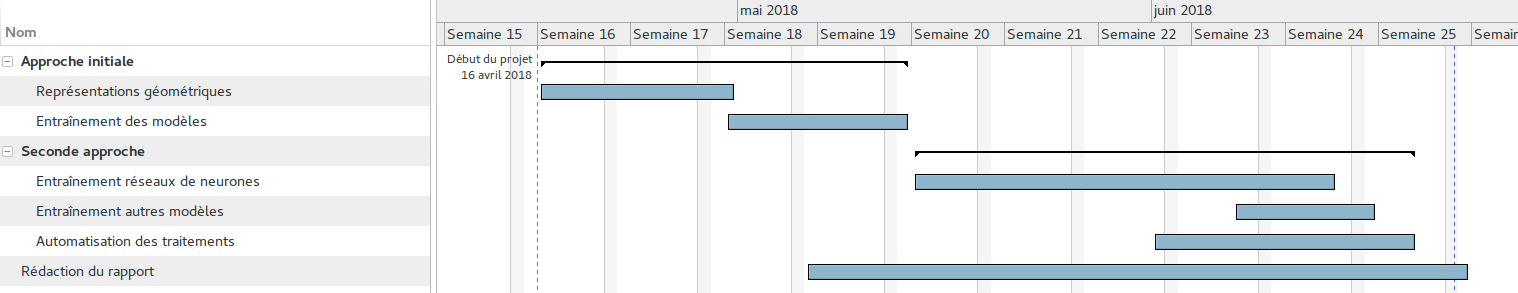
\includegraphics[scale=0.45]{images/gantt.png}	
	
	\caption{Diagramme de Gantt des grandes étapes du travail (Généré avec le programme Planner)}
\end{figure}

\end{landscape}


\chapter{Représentations graphiques des prédictions des modèles \emph{DIST\_REL\_C}}

\label{annexes_plots_dist_rel_c}

\begin{figure}[!h]
	\centering
	
	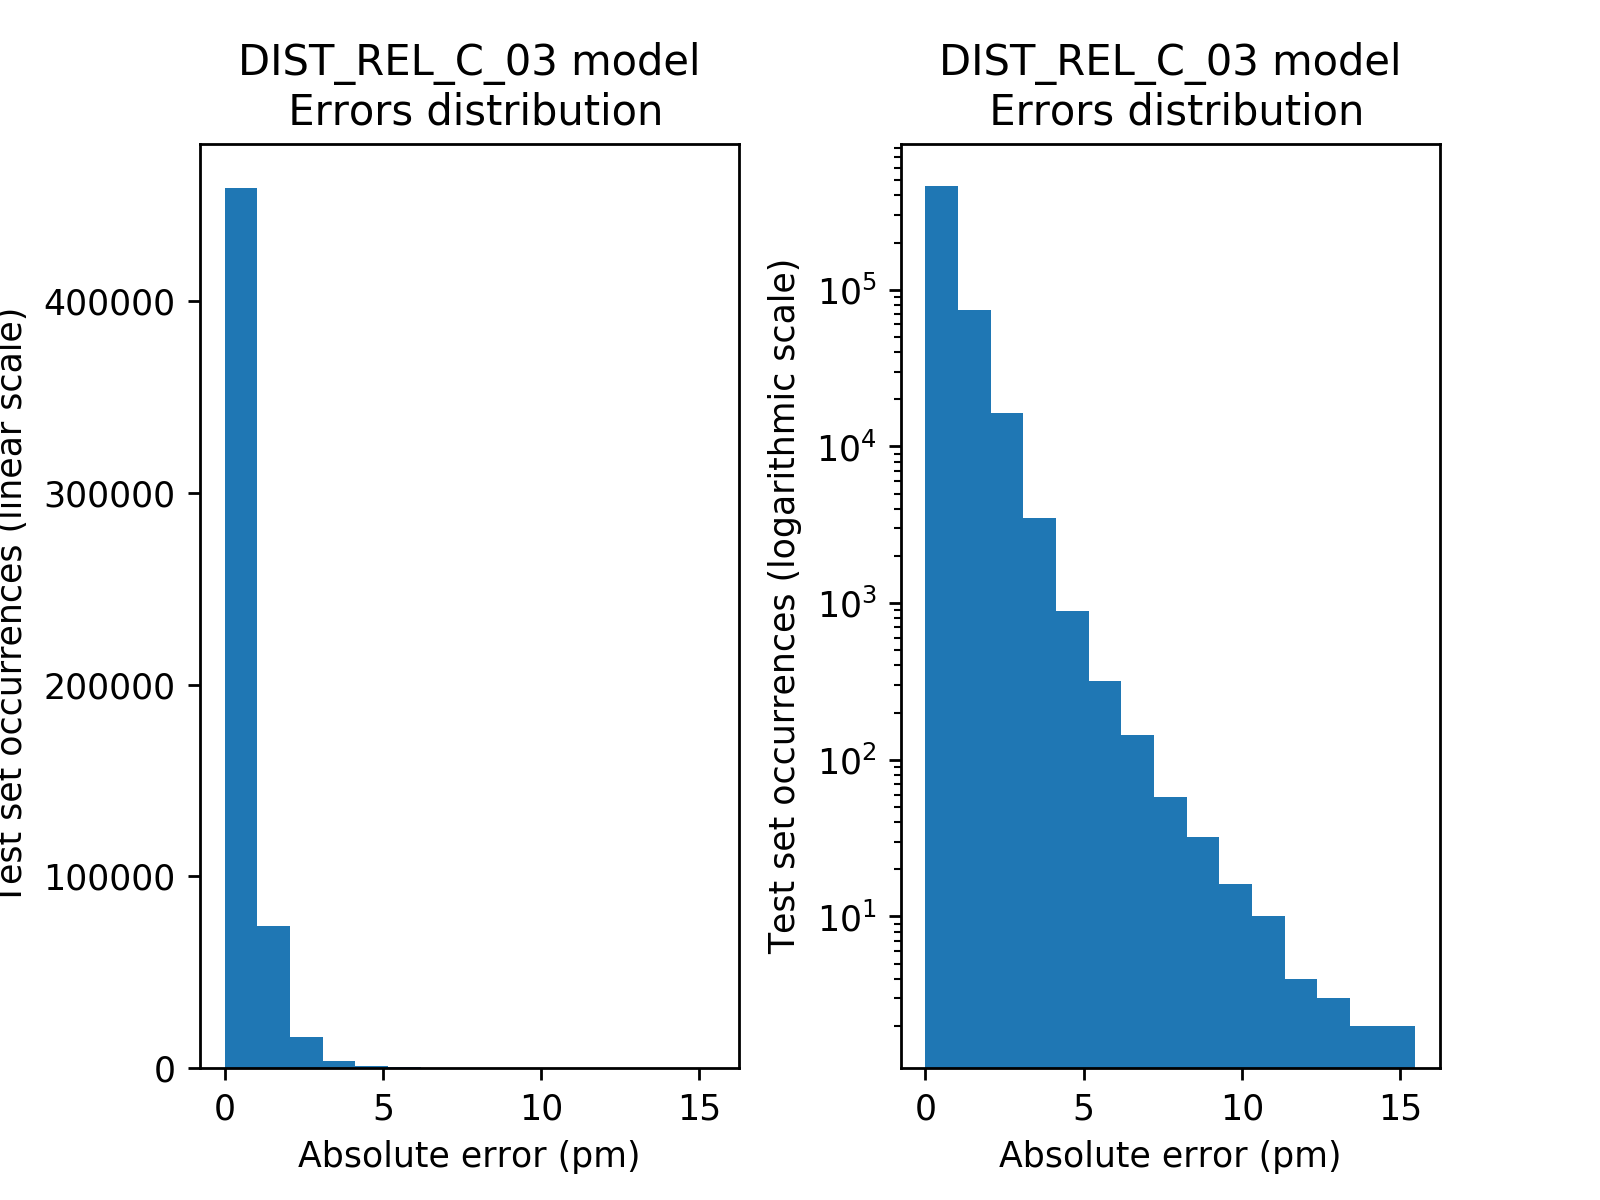
\includegraphics[scale=0.75]{../figures/DIST_REL_C_03/DIST_REL_C_03_distrib_rmse_val.png}	
	
	\caption{Distribution des erreurs du modèle \emph{DIST\_REL\_C\_03}. Modèle s'entraînant sur une \textbf{quantité modérée d'exemples} et prédisant les longueurs de liaisons \textbf{carbone-carbone}, à partir de données d'entrées sur lesquelles la \textbf{fonction inverse} a été appliquée aux distances, \textbf{avec restriction} au voisinage le plus proche.}
\end{figure}
\begin{figure}[!h]
	\centering
	
	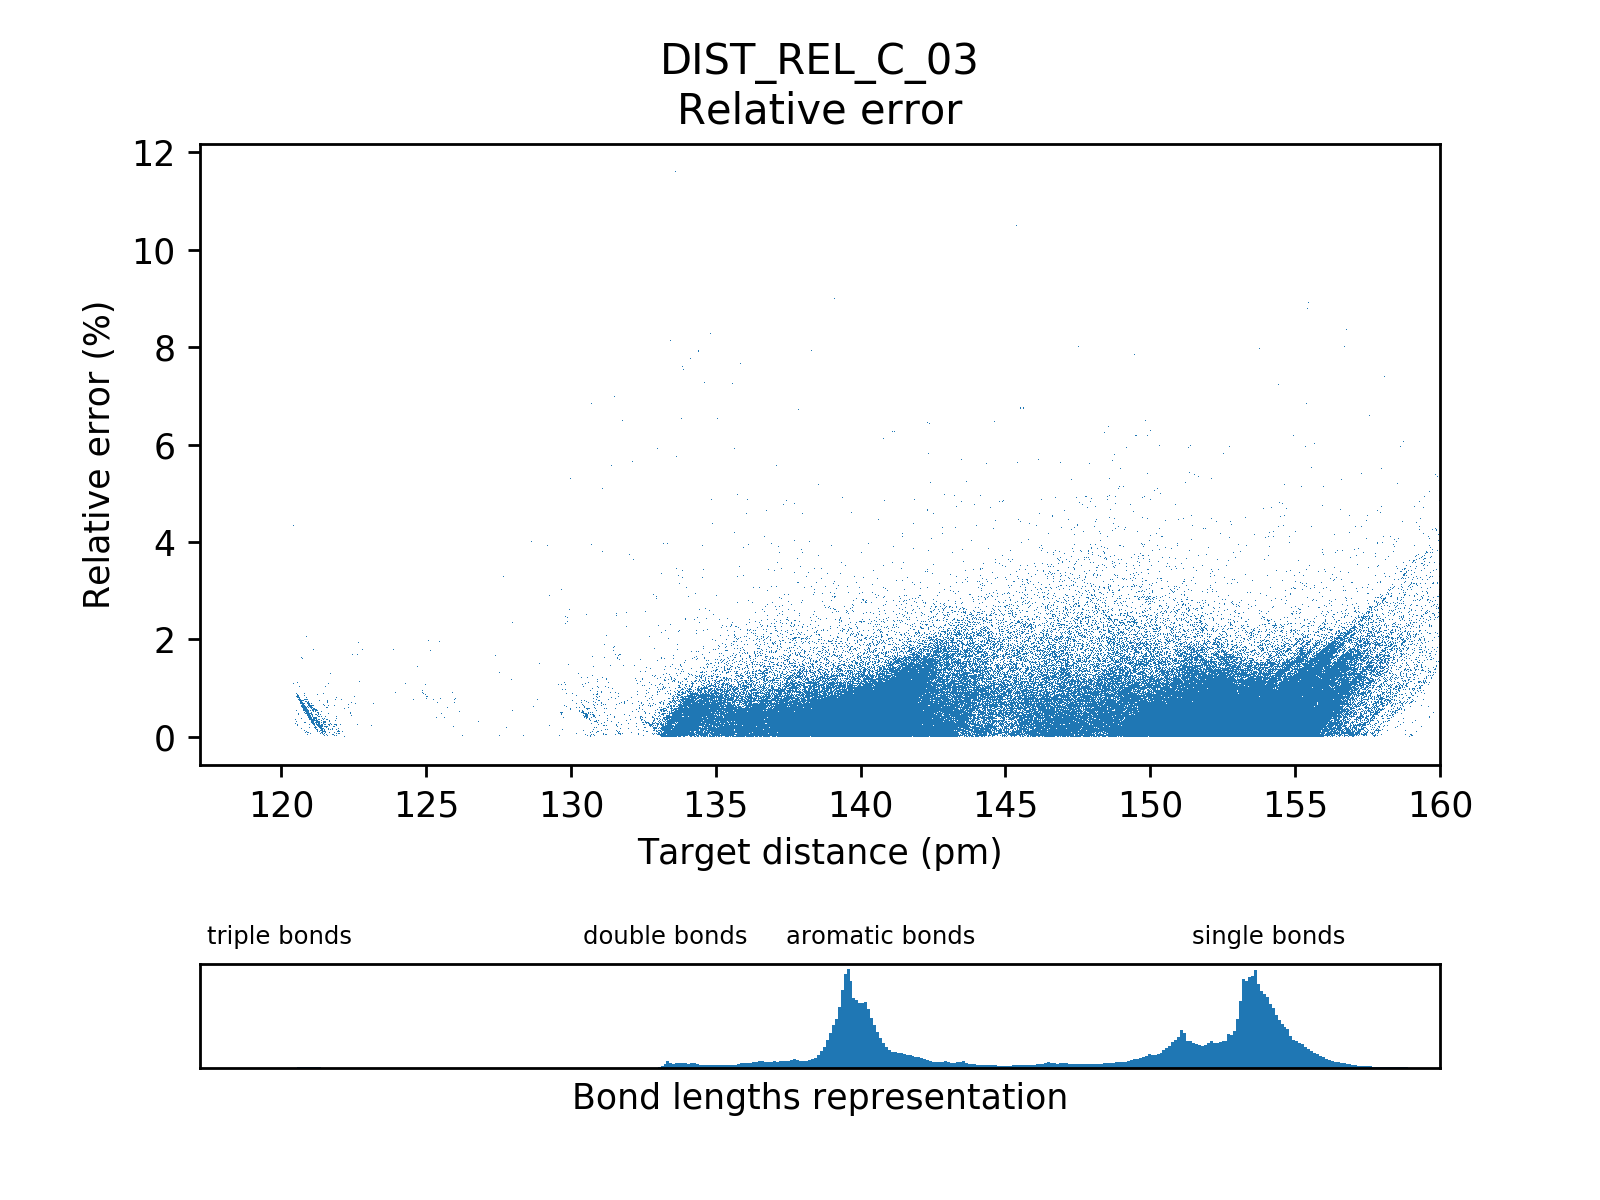
\includegraphics[scale=0.75]{../figures/DIST_REL_C_03/DIST_REL_C_03_distrib_rmse_dist.png}	
	
	\caption{Erreur en fonction des cibles pour le modèle \emph{DIST\_REL\_C\_03}. Modèle s'entraînant sur une \textbf{quantité modérée d'exemples} et prédisant les longueurs de liaisons \textbf{carbone-carbone}, à partir de données d'entrées sur lesquelles la \textbf{fonction inverse} a été appliquée aux distances, \textbf{avec restriction} au voisinage le plus proche.}
	\end{figure}

\begin{figure}[!h]
	\centering
	
	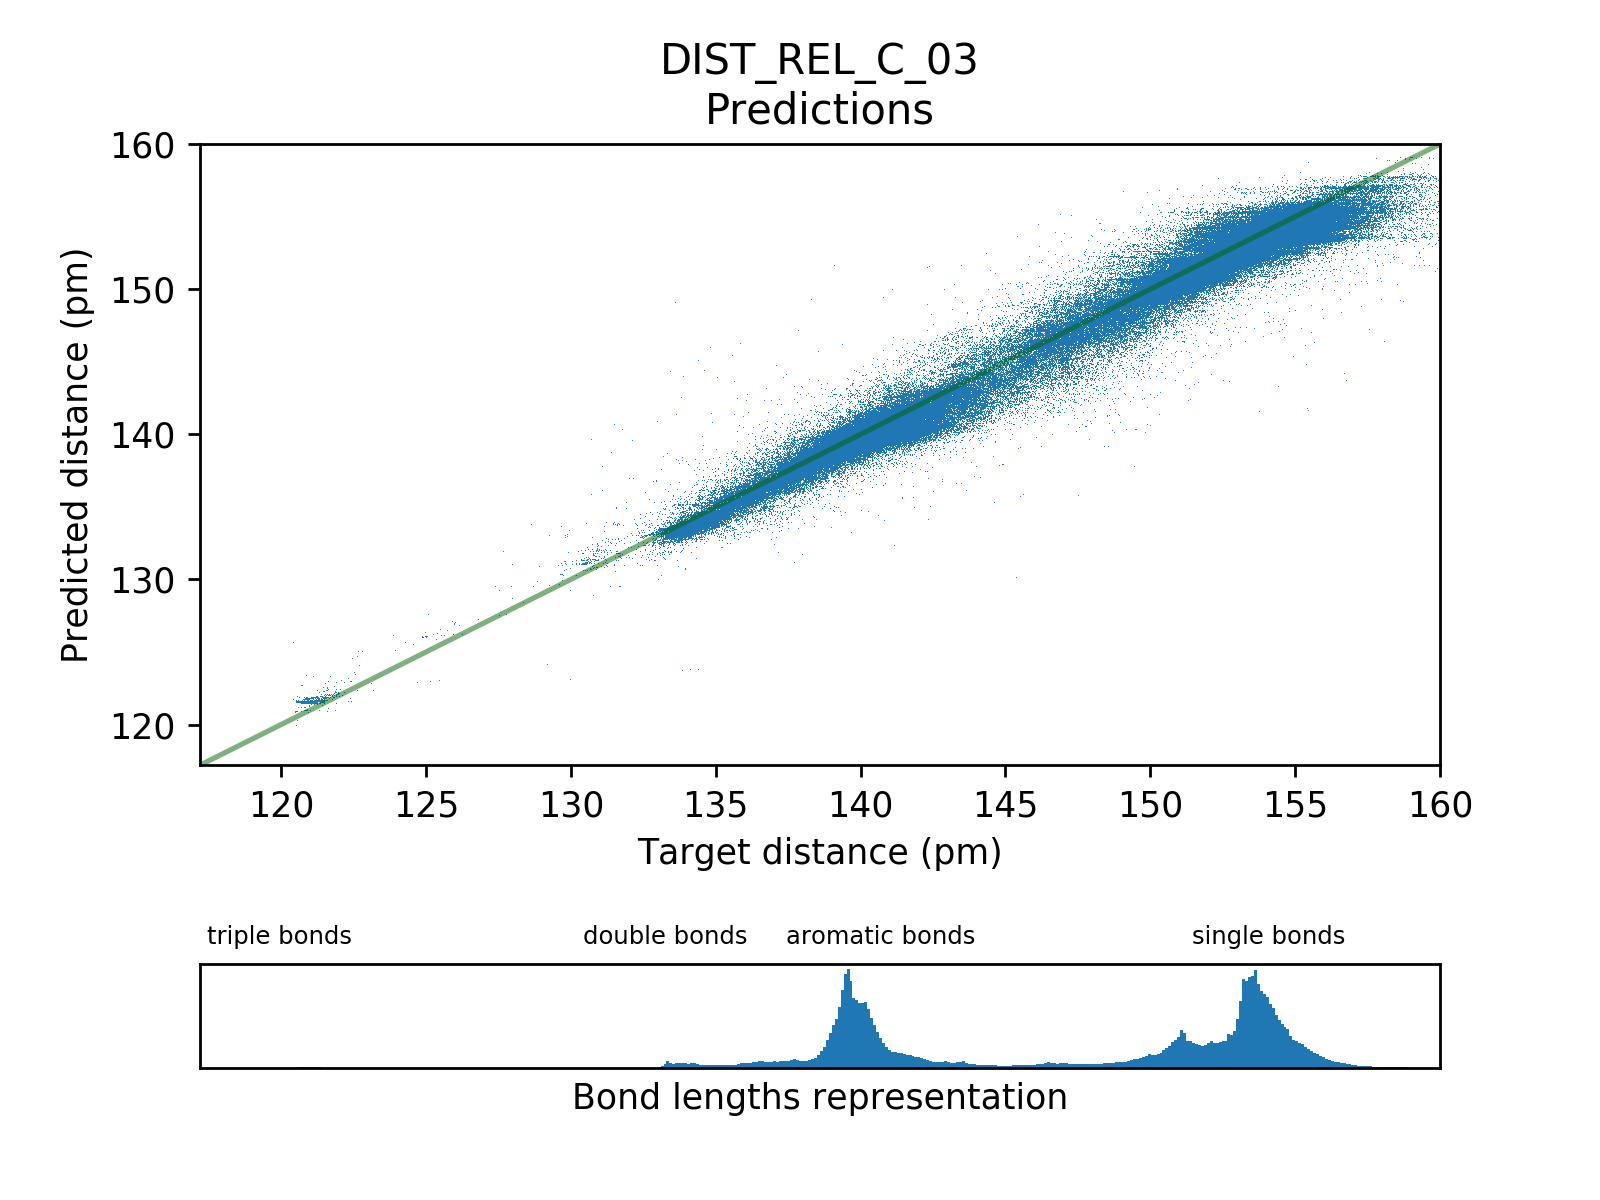
\includegraphics[scale=0.75]{../figures/DIST_REL_C_03/DIST_REL_C_03_preds_targets.png}	
	
	\caption{Prédictions en fonction des cibles pour le modèle \emph{DIST\_REL\_C\_03}. Modèle s'entraînant sur une \textbf{quantité modérée d'exemples} et prédisant les longueurs de liaisons \textbf{carbone-carbone}, à partir de données d'entrées sur lesquelles la \textbf{fonction inverse} a été appliquée aux distances, \textbf{avec restriction} au voisinage le plus proche.}
	
\end{figure}

\begin{figure}[!h]
	\centering
	
	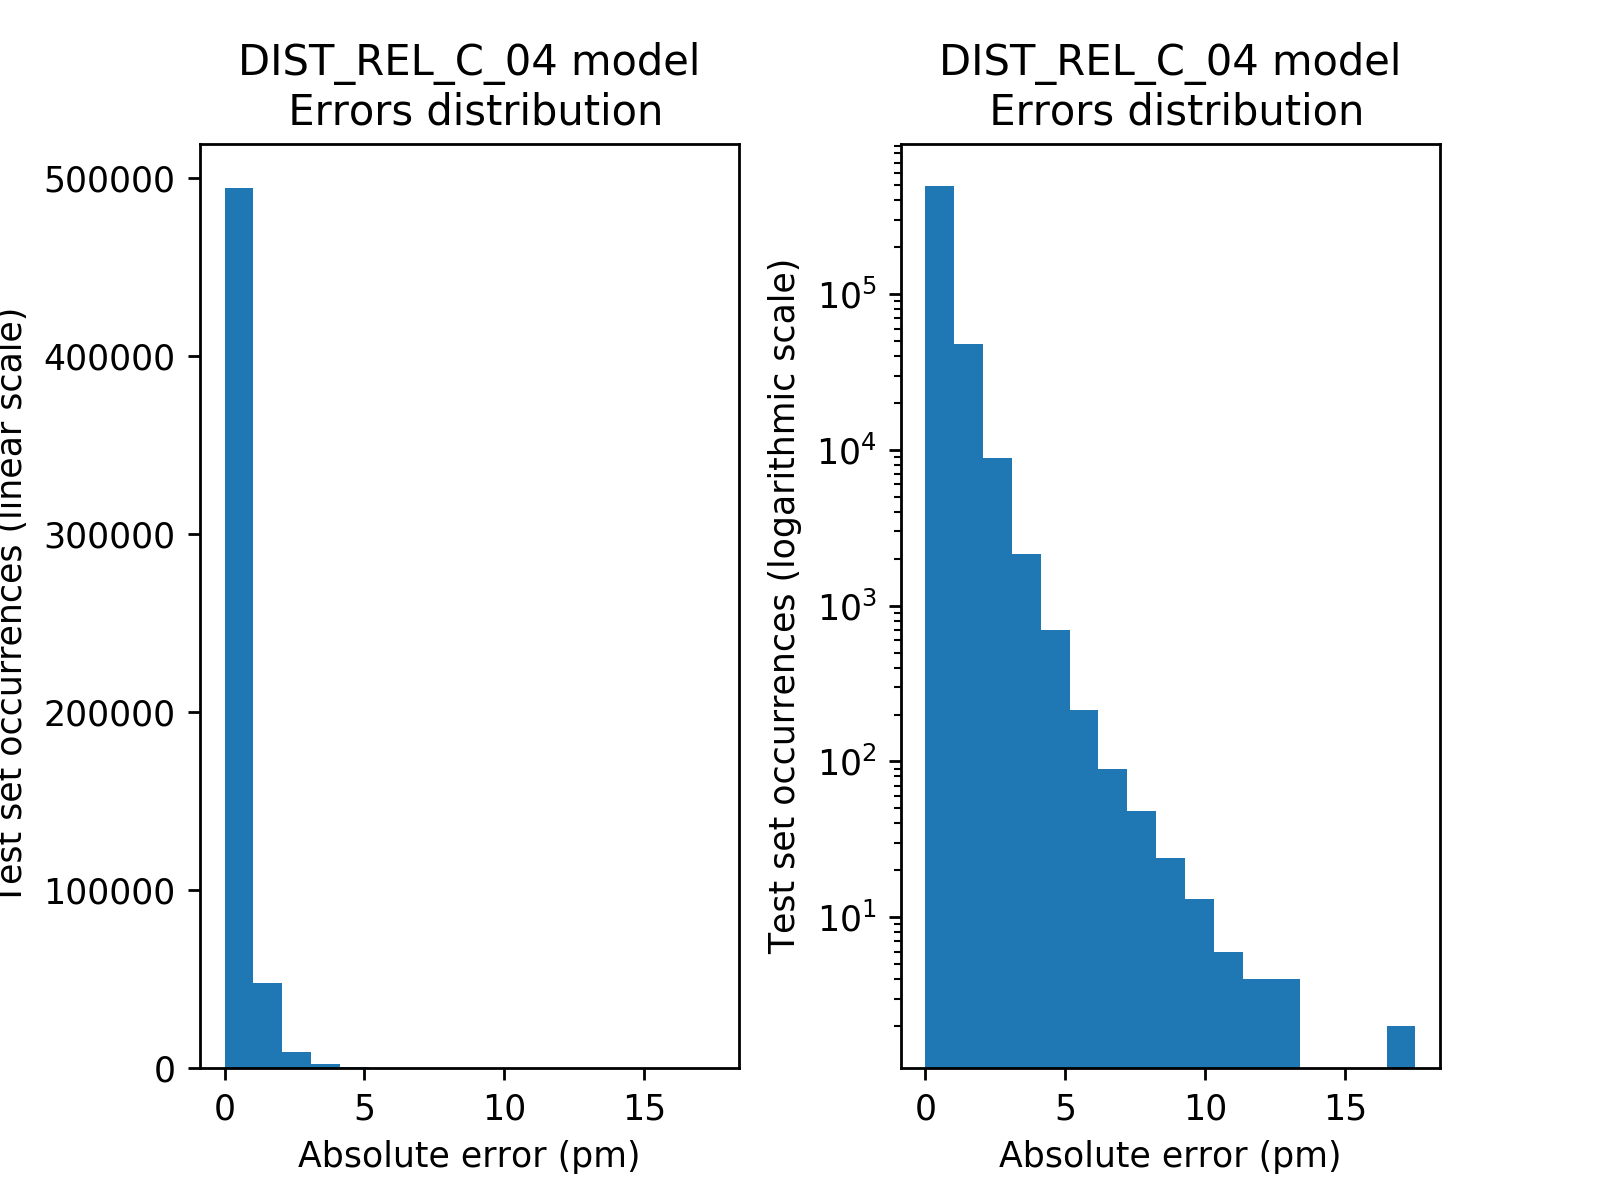
\includegraphics[scale=0.75]{../figures/DIST_REL_C_04/DIST_REL_C_04_distrib_rmse_val.png}	
	
	\caption{Distribution des erreurs du modèle \emph{DIST\_REL\_C\_04}. Modèle s'entraînant sur une \textbf{quantité modérée d'exemples} et prédisant les longueurs de liaisons \textbf{carbone-carbone}, à partir de données d'entrées sur lesquelles la \textbf{fonction inverse du carré} a été appliquée aux distances, \textbf{avec restriction} au voisinage le plus proche.}
\end{figure}
\begin{figure}[!h]
	\centering
	
	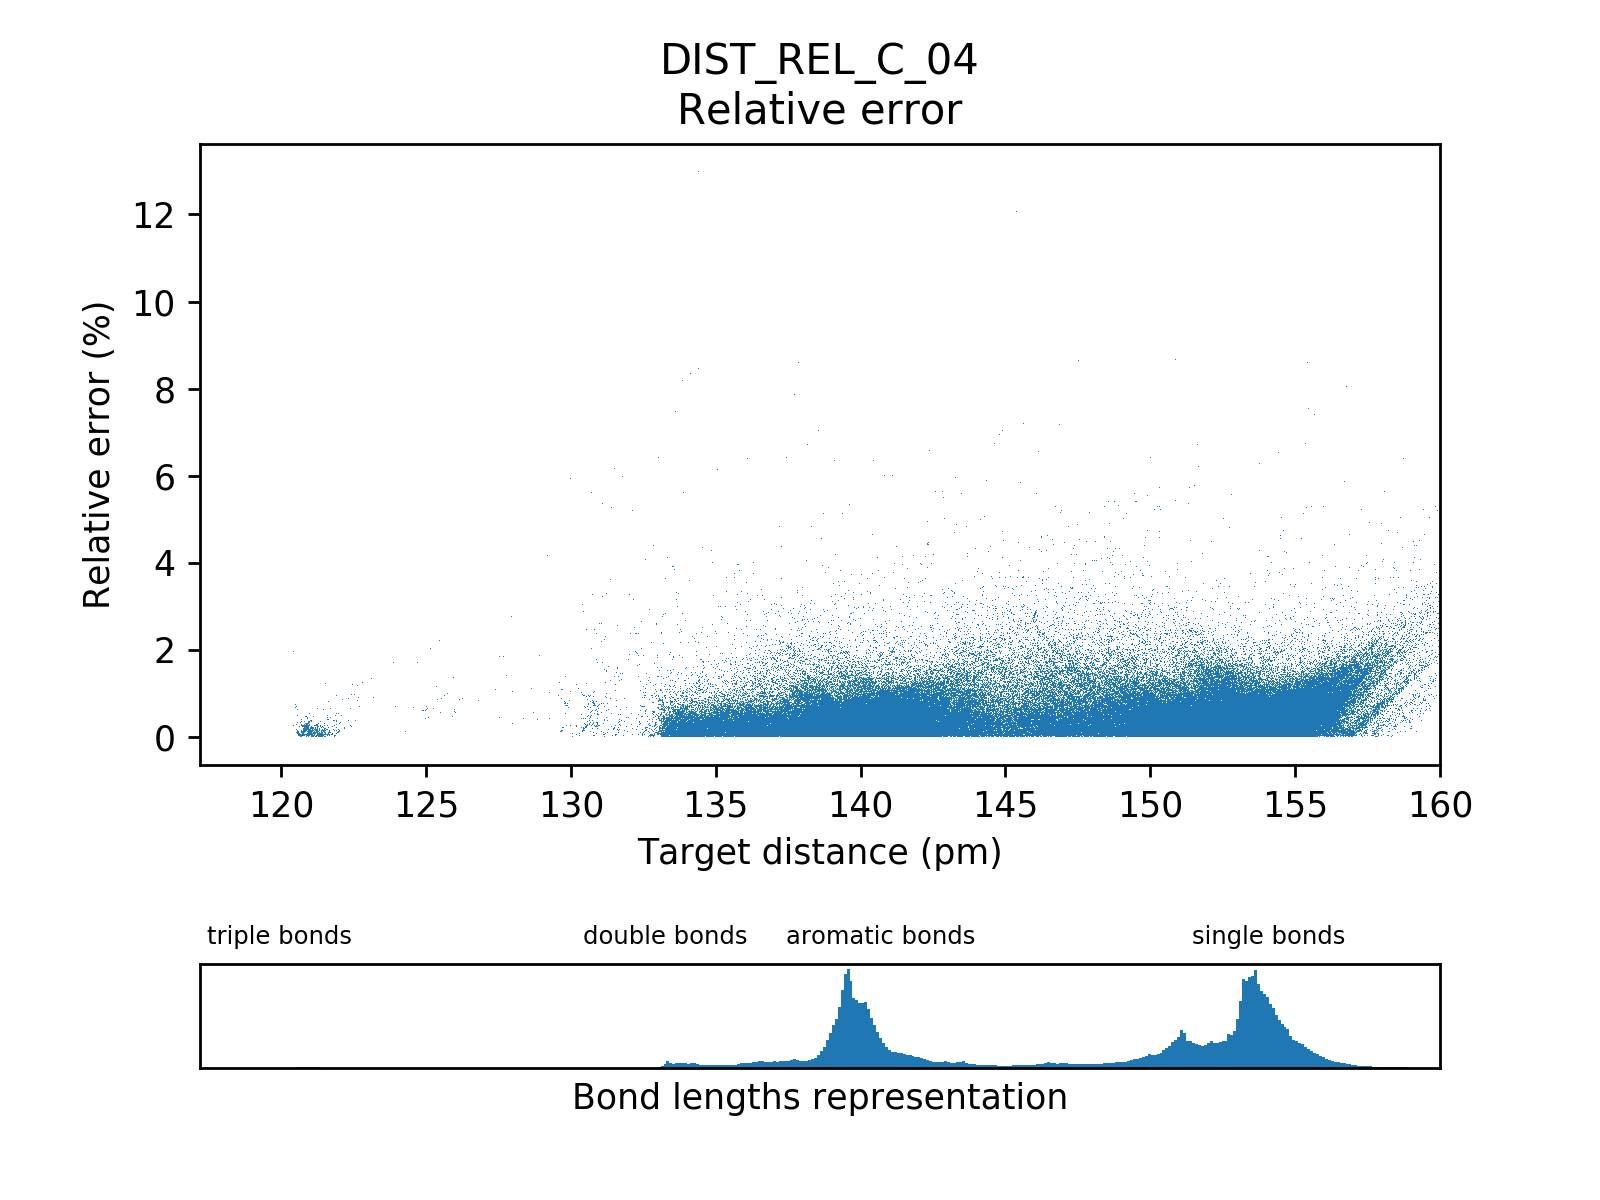
\includegraphics[scale=0.75]{../figures/DIST_REL_C_04/DIST_REL_C_04_distrib_rmse_dist.png}	
	
	\caption{Erreur en fonction des cibles pour le modèle \emph{DIST\_REL\_C\_04}. Modèle s'entraînant sur une \textbf{quantité modérée d'exemples} et prédisant les longueurs de liaisons \textbf{carbone-carbone}, à partir de données d'entrées sur lesquelles la \textbf{fonction inverse du carré} a été appliquée aux distances, \textbf{avec restriction} au voisinage le plus proche.}
	\end{figure}

\begin{figure}[!h]
	\centering
	
	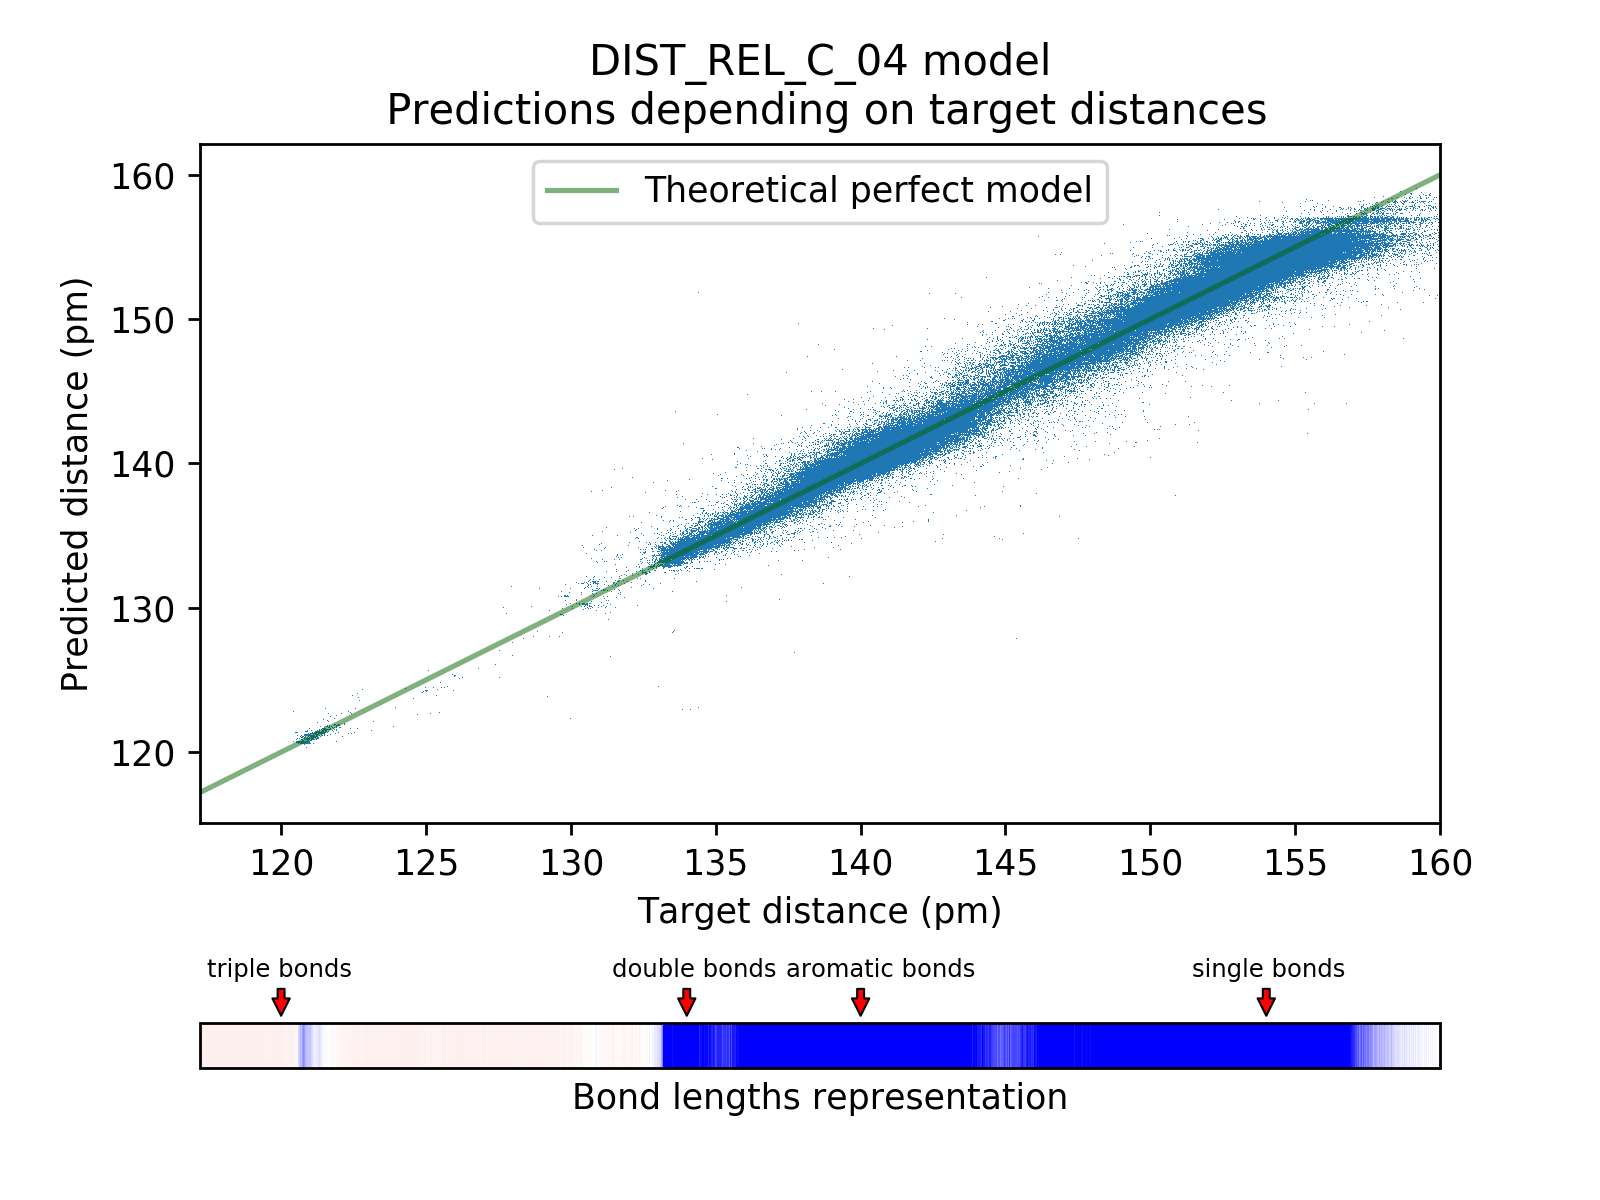
\includegraphics[scale=0.75]{../figures/DIST_REL_C_04/DIST_REL_C_04_preds_targets.png}	
	
	\caption{Prédictions en fonction des cibles pour le modèle \emph{DIST\_REL\_C\_04}. Modèle s'entraînant sur une \textbf{quantité modérée d'exemples} et prédisant les longueurs de liaisons \textbf{carbone-carbone}, à partir de données d'entrées sur lesquelles la \textbf{fonction inverse du carré} a été appliquée aux distances, \textbf{avec restriction} au voisinage le plus proche.}
	
\end{figure}


\chapter{Représentations graphiques des prédictions des modèles \emph{DIST\_REL\_XY}}

\label{annexes_plot_dist_rel_xy}

% DIST REL CC_01
\begin{figure}[!h]
	\centering
	
	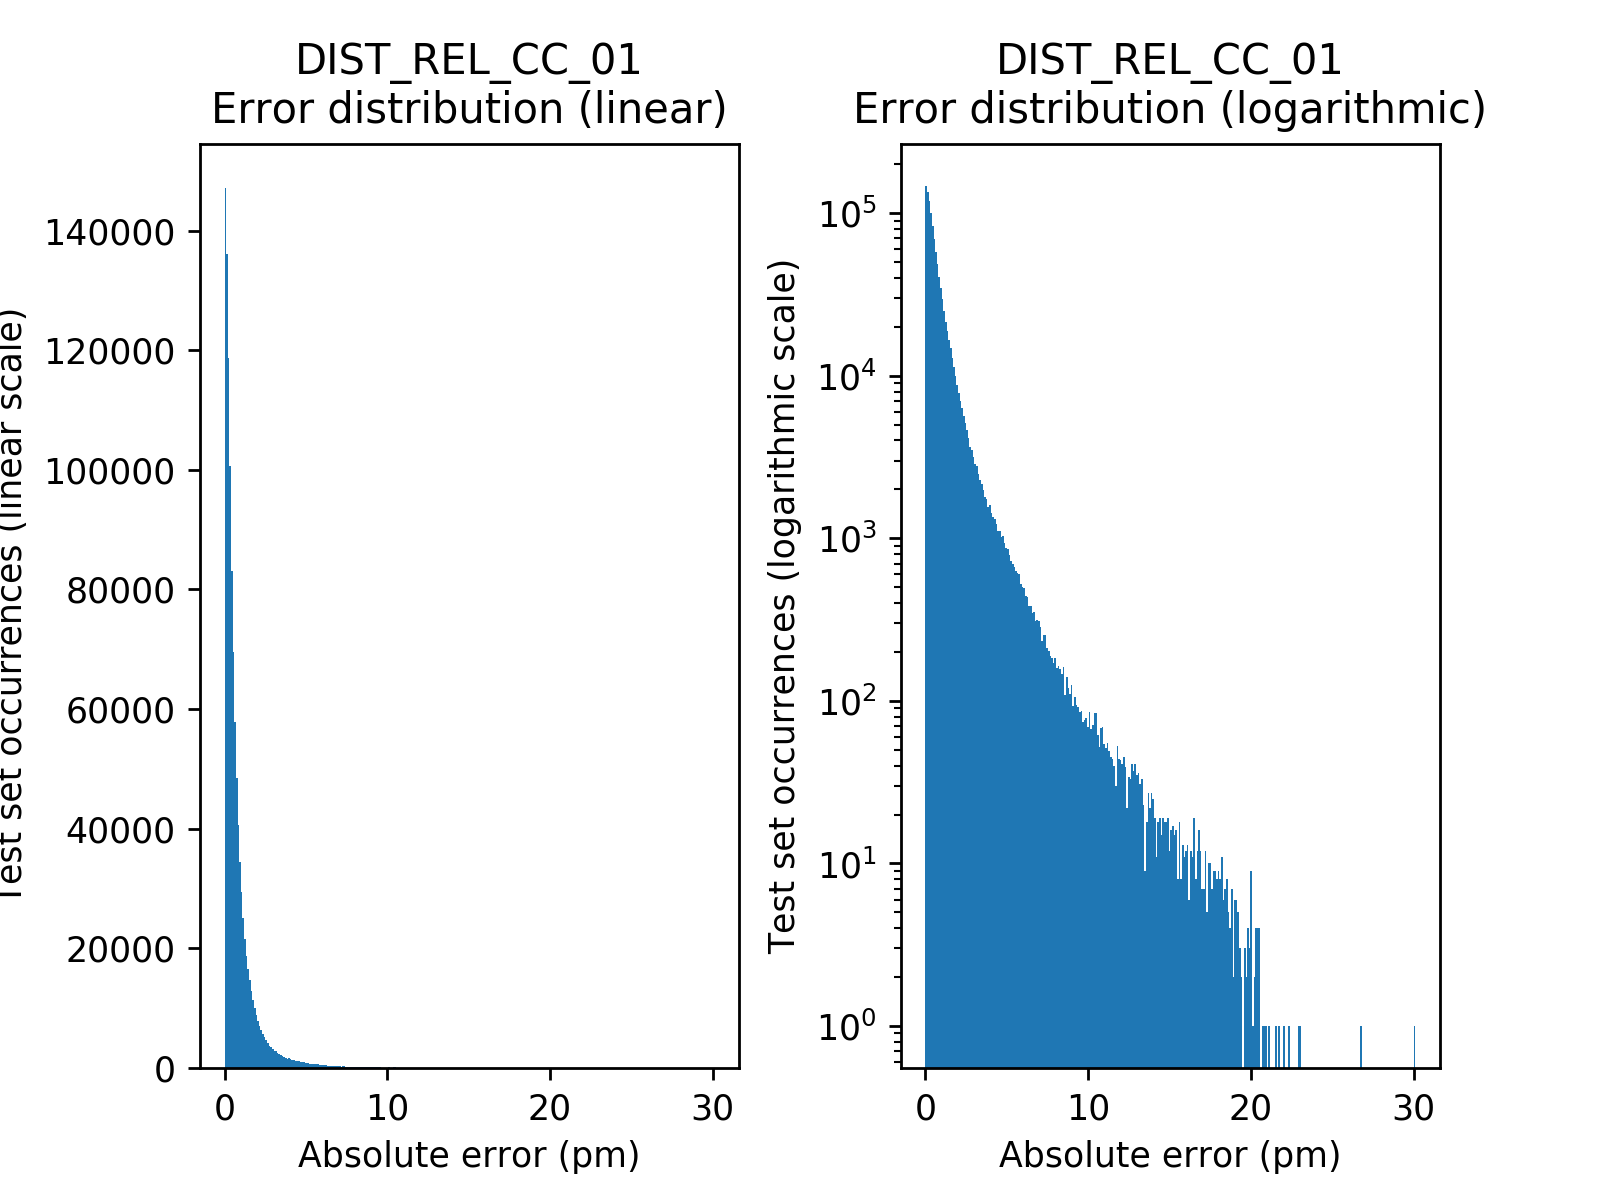
\includegraphics[scale=0.75]{../figures/DIST_REL_CC_01/DIST_REL_CC_01_distrib_rmse_val.png}	
	
	\caption{Distribution des erreurs du modèle \emph{DIST\_REL\_CC\_01}. Modèle s'entraînant sur une \textbf{grande quantité d'exemples} et prédisant les longueurs de liaisons \textbf{carbone-carbone}, à partir de données d'entrées sur lesquelles \textbf{aucune fonction} n'a été appliquée aux distances, \textbf{sans restriction} au voisinage le plus proche.}
\end{figure}
\begin{figure}[!h]
	\centering
	
	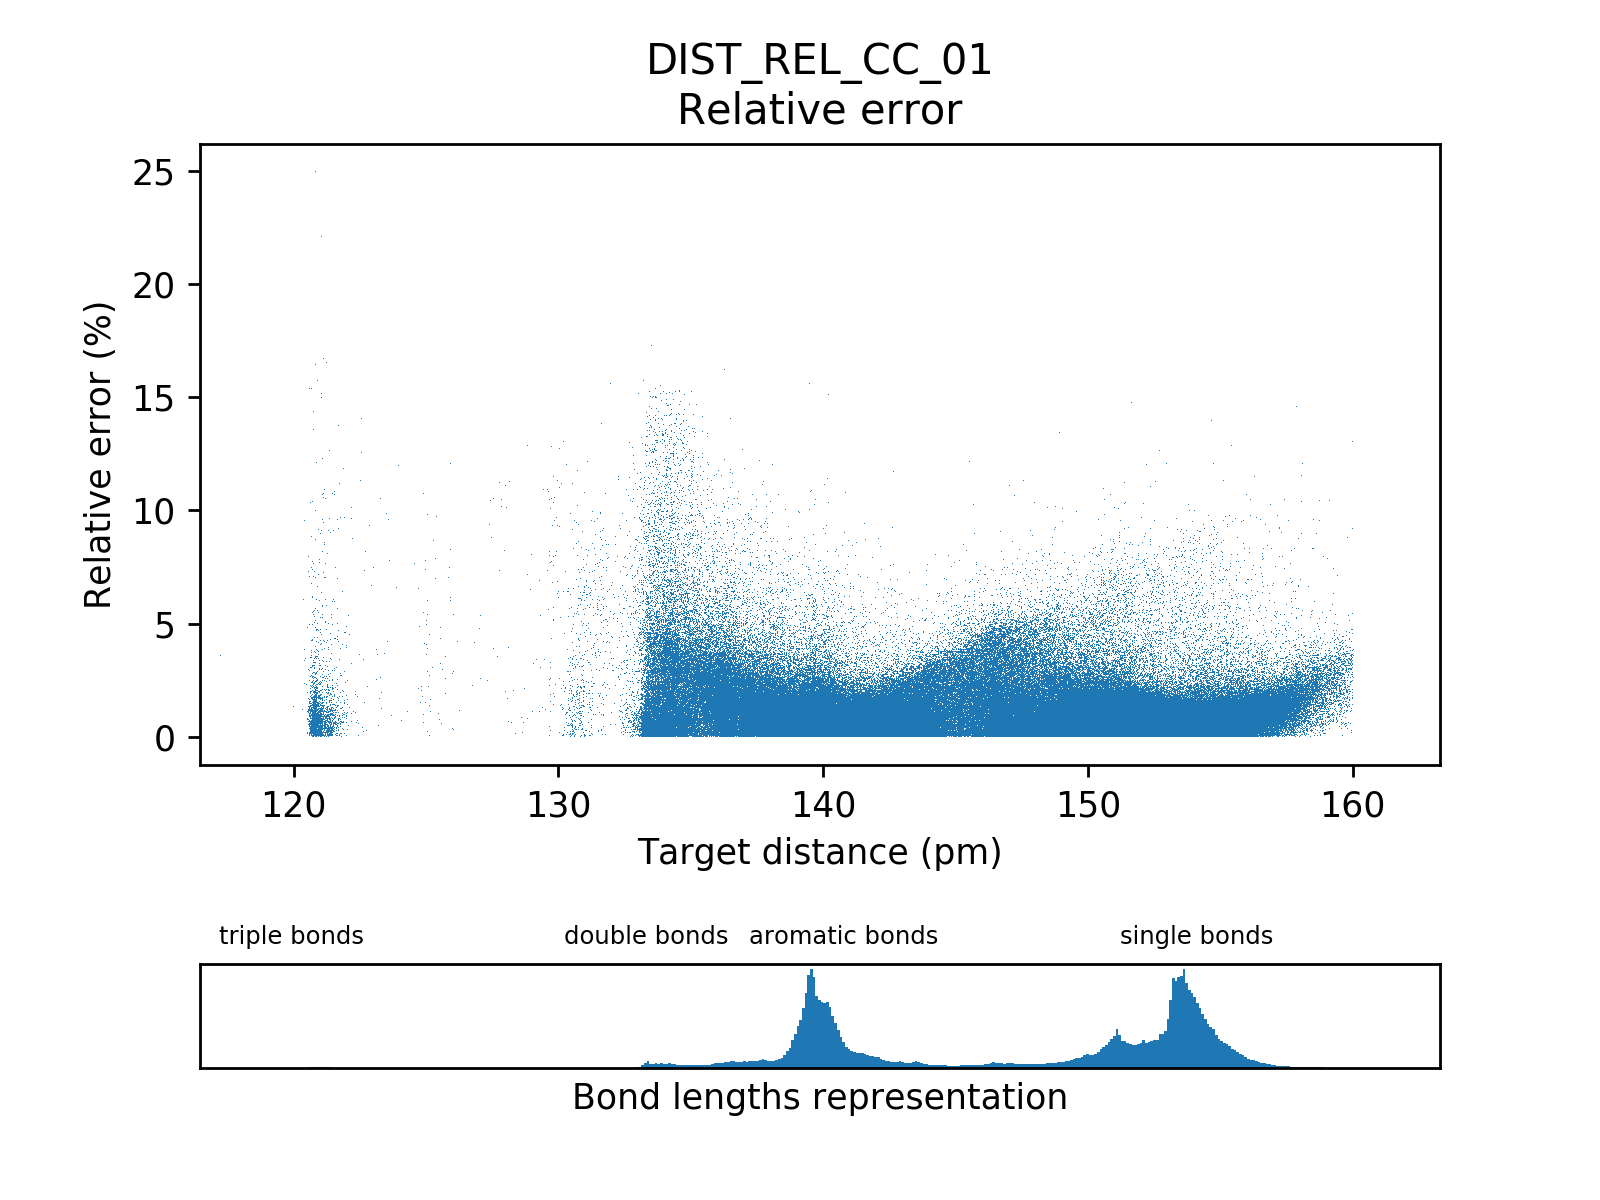
\includegraphics[scale=0.75]{../figures/DIST_REL_CC_01/DIST_REL_CC_01_distrib_rmse_dist.png}	
	
	\caption{Erreur en fonction des cibles pour le modèle \emph{DIST\_REL\_CC\_01}. Modèle s'entraînant sur une \textbf{grande quantité d'exemples} et prédisant les longueurs de liaisons \textbf{carbone-carbone}, à partir de données d'entrées sur lesquelles \textbf{aucune fonction} n'a été appliquée aux distances, \textbf{sans restriction} au voisinage le plus proche.}
	\end{figure}

\begin{figure}[!h]
	\centering
	
	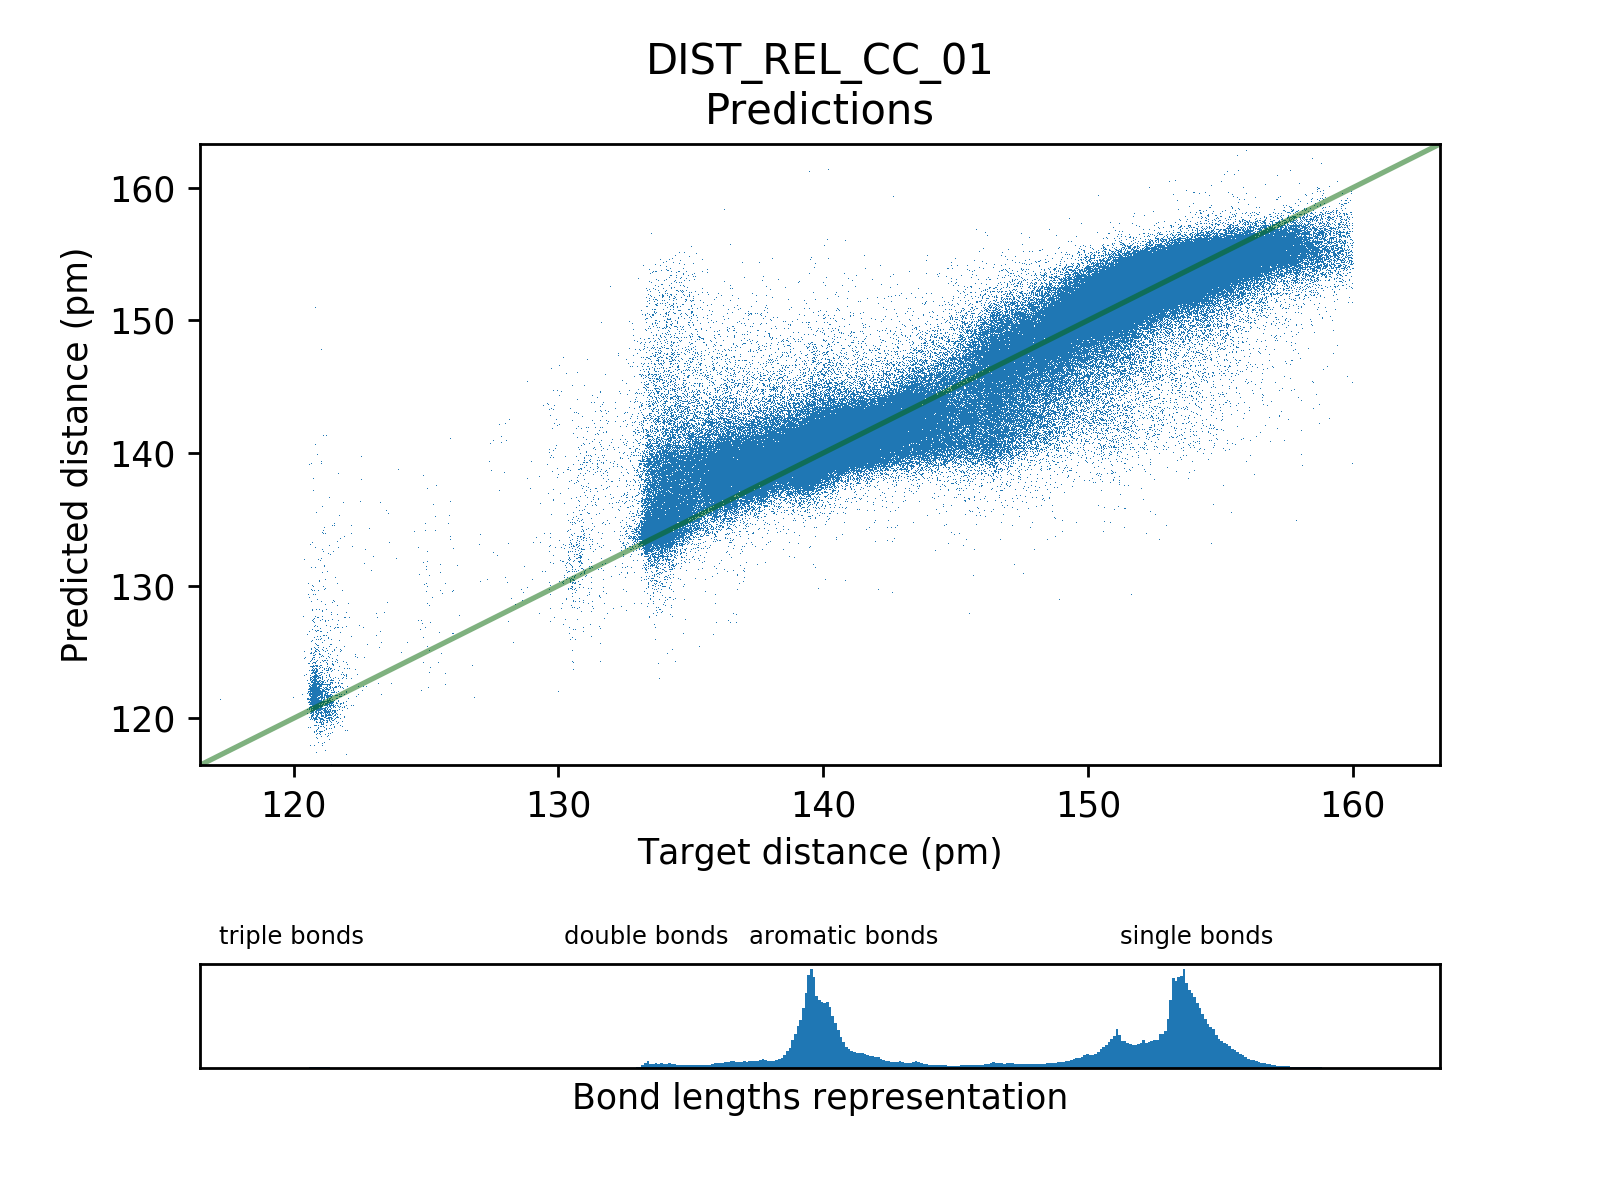
\includegraphics[scale=0.75]{../figures/DIST_REL_CC_01/DIST_REL_CC_01_preds_targets.png}	
	
	\caption{Prédictions en fonction des cibles pour le modèle \emph{DIST\_REL\_CC\_01}. Modèle s'entraînant sur une \textbf{grande quantité d'exemples} et prédisant les longueurs de liaisons \textbf{carbone-carbone}, à partir de données d'entrées sur lesquelles \textbf{aucune fonction} n'a été appliquée aux distances, \textbf{sans restriction} au voisinage le plus proche.}
	
\end{figure}


% DIST REL OH_02

\begin{figure}[!h]
	\centering
	
	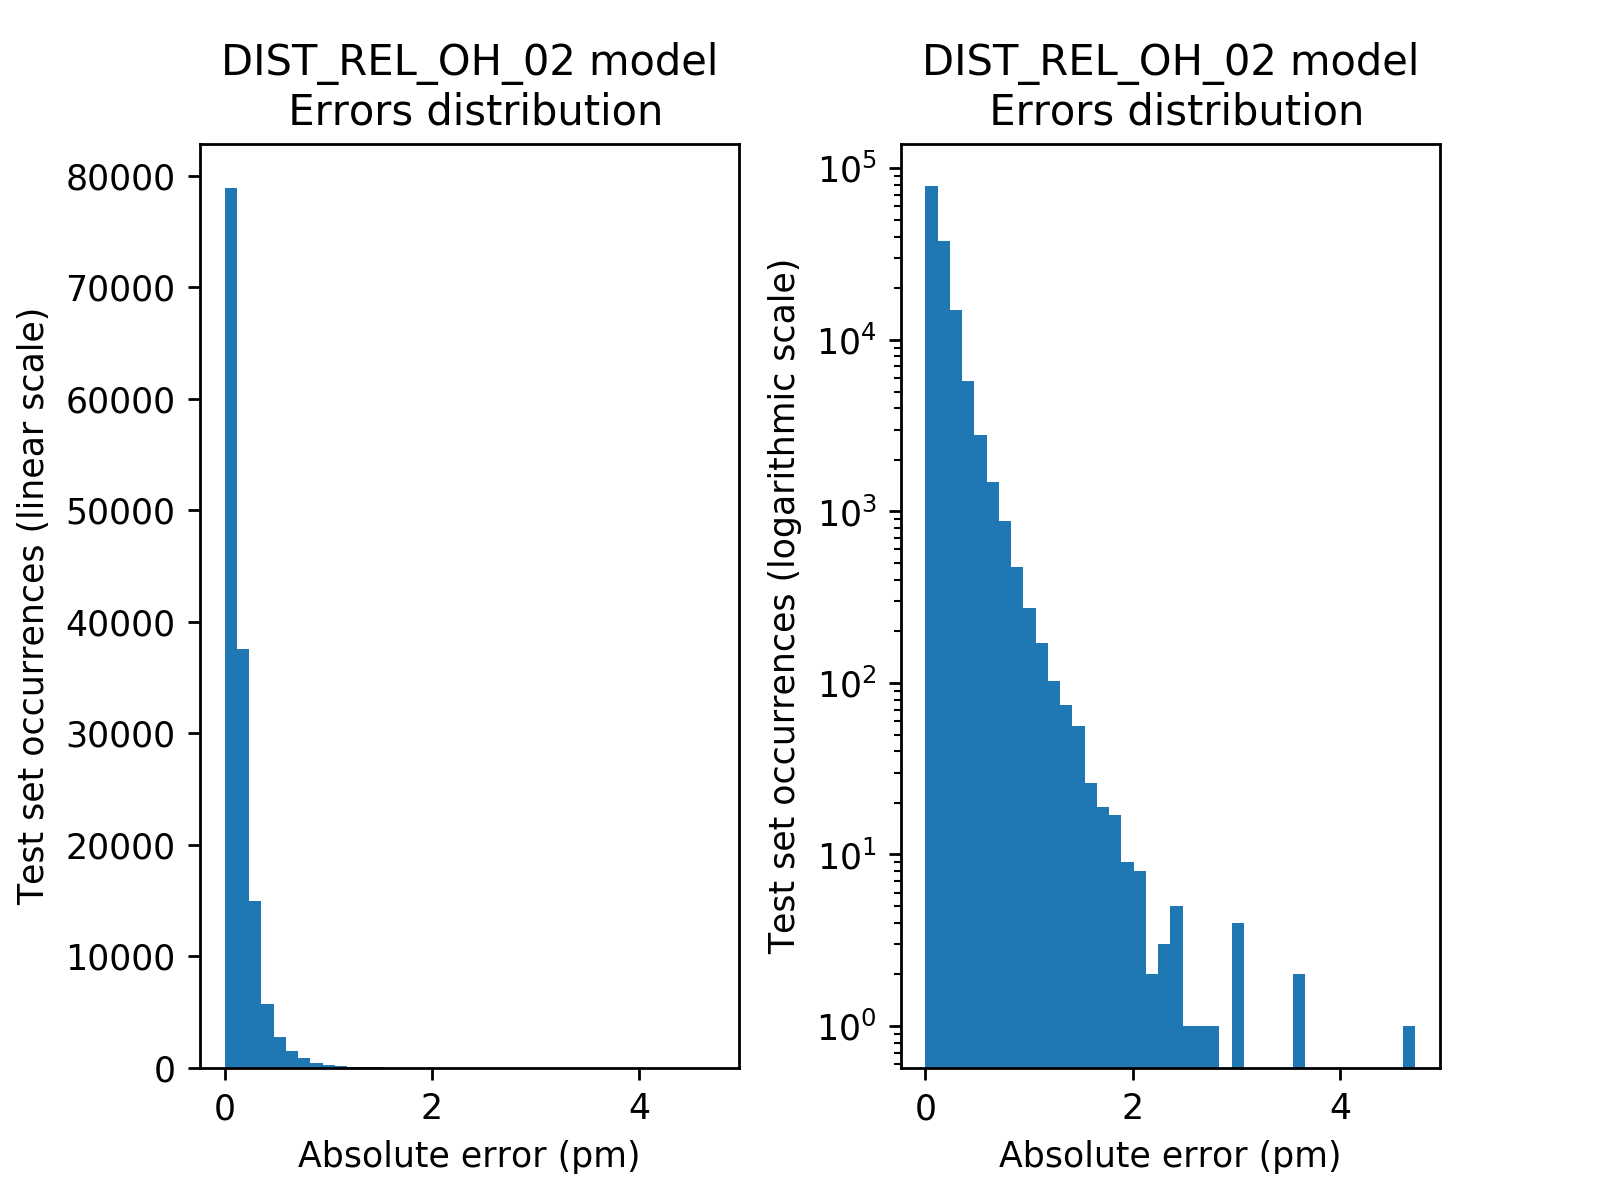
\includegraphics[scale=0.75]{../figures/DIST_REL_OH_02/DIST_REL_OH_02_distrib_rmse_val.png}	
	
	\caption{Distribution des erreurs du modèle \emph{DIST\_REL\_OH\_02}. Modèle s'entraînant sur une \textbf{grande quantité d'exemples} et prédisant les longueurs de liaisons \textbf{oxygène-hydrogène}, à partir de données d'entrées sur lesquelles \textbf{aucune fonction} n'a été appliquée aux distances, \textbf{avec restriction} au voisinage le plus proche.}
\end{figure}
\begin{figure}[!h]
	\centering
	
	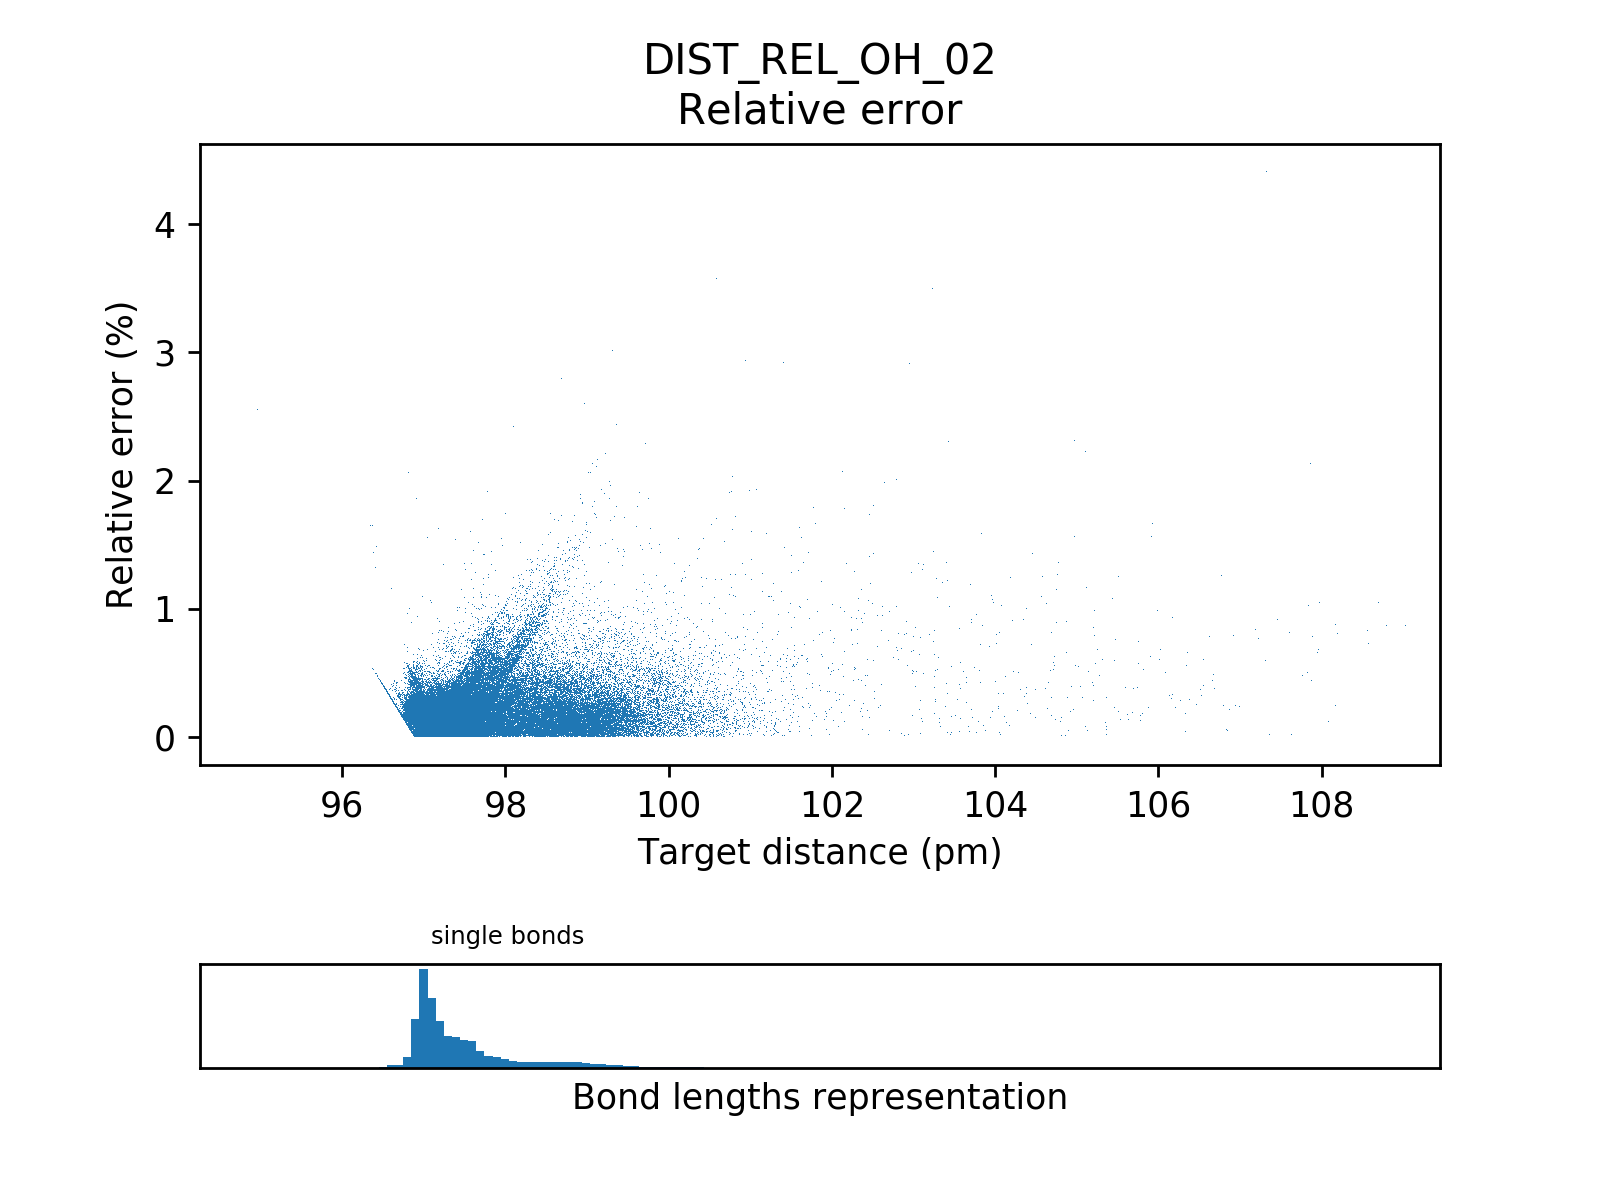
\includegraphics[scale=0.75]{../figures/DIST_REL_OH_02/DIST_REL_OH_02_distrib_rmse_dist.png}	
	
	\caption{Erreur en fonction des cibles pour le modèle \emph{DIST\_REL\_OH\_02}. Modèle s'entraînant sur une \textbf{grande quantité d'exemples} et prédisant les longueurs de liaisons \textbf{oxygène-hydrogène}, à partir de données d'entrées sur lesquelles \textbf{aucune fonction} n'a été appliquée aux distances, \textbf{avec restriction} au voisinage le plus proche.}
	\end{figure}

\begin{figure}[!h]
	\centering
	
	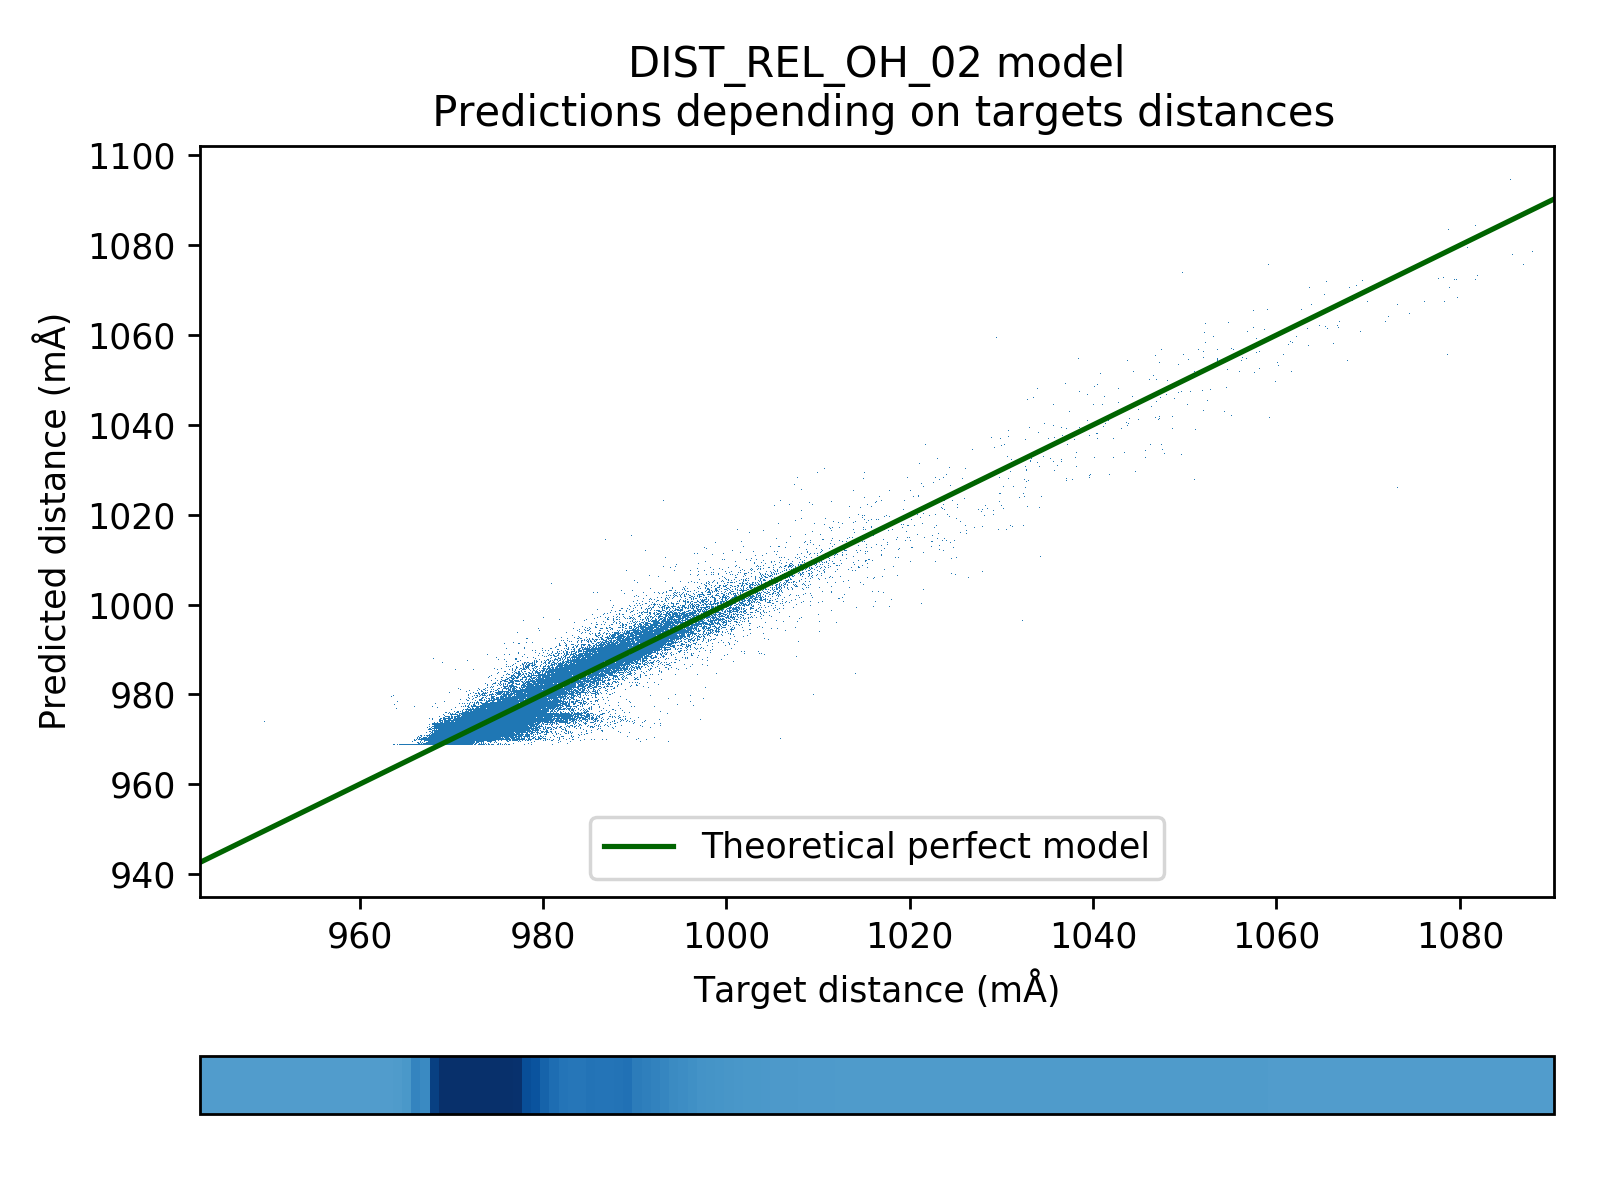
\includegraphics[scale=0.75]{../figures/DIST_REL_OH_02/DIST_REL_OH_02_preds_targets.png}	
	
	\caption{Prédictions en fonction des cibles pour le modèle \emph{DIST\_REL\_OH\_02}. Modèle s'entraînant sur une \textbf{grande quantité d'exemples} et prédisant les longueurs de liaisons \textbf{oxygène-hydrogène}, à partir de données d'entrées sur lesquelles \textbf{aucune fonction} n'a été appliquée aux distances, \textbf{avec restriction} au voisinage le plus proche.}
	
\end{figure}
	
	
% DIST REL CH 02

\begin{figure}[!h]
	\centering
	
	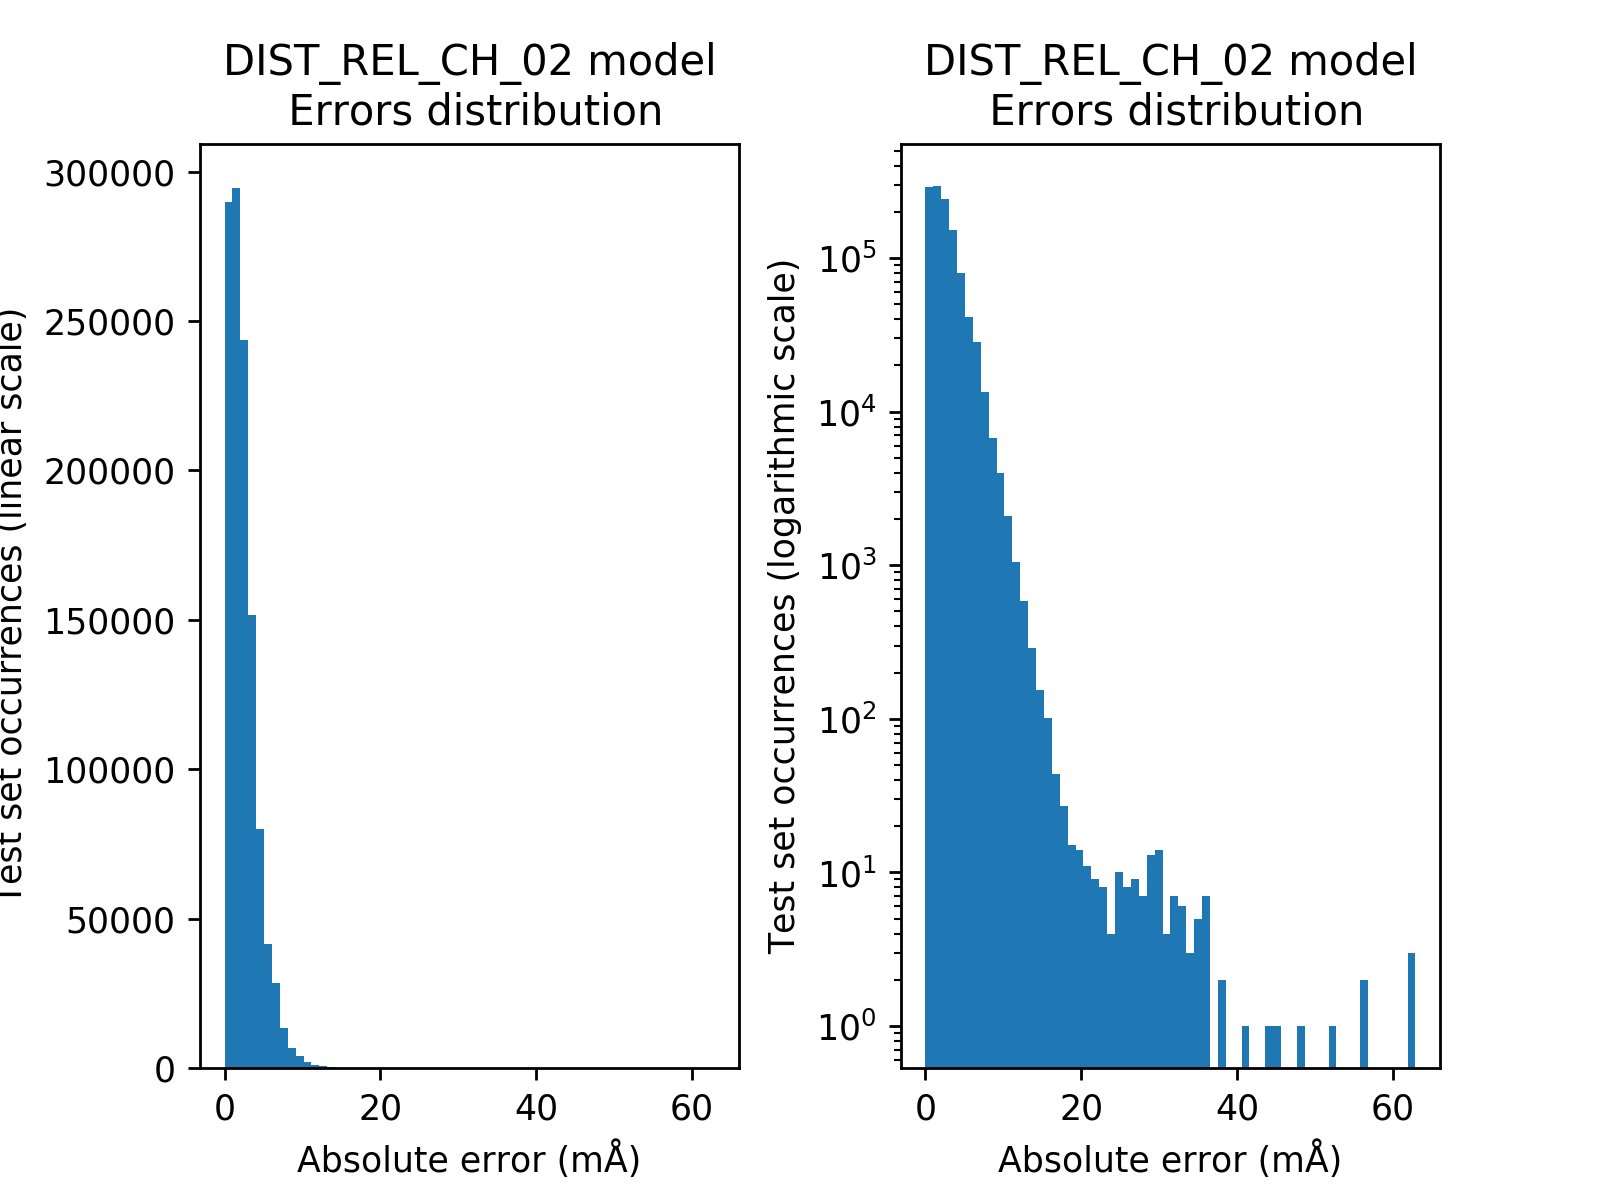
\includegraphics[scale=0.75]{../figures/DIST_REL_CH_02/DIST_REL_CH_02_distrib_rmse_val.png}	
	
	\caption{Distribution des erreurs du modèle \emph{DIST\_REL\_CH\_02}. Modèle s'entraînant sur une \textbf{grande quantité d'exemples} et prédisant les longueurs de liaisons \textbf{carbone-hydrogène}, à partir de données d'entrées sur lesquelles \textbf{aucune fonction} n'a été appliquée aux distances, \textbf{avec restriction} au voisinage le plus proche.}
\end{figure}

\begin{figure}[!h]
	\centering
	
	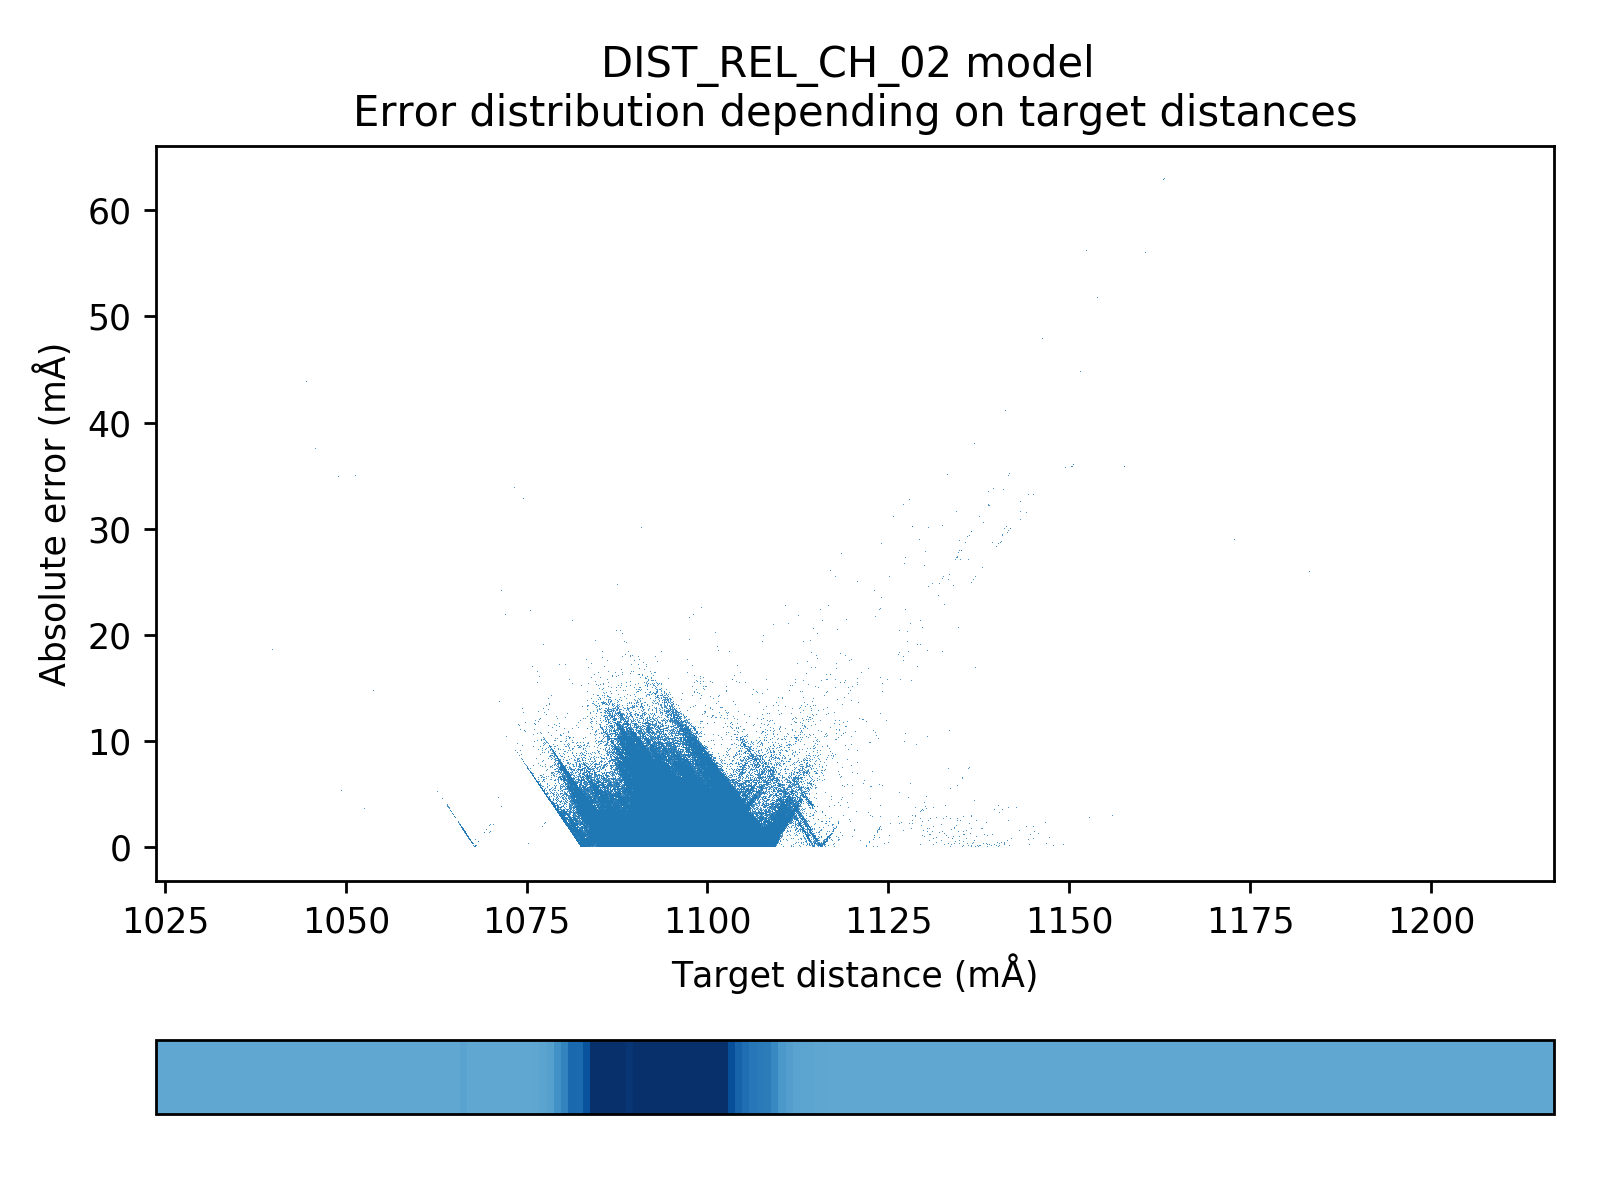
\includegraphics[scale=0.75]{../figures/DIST_REL_CH_02/DIST_REL_CH_02_distrib_rmse_dist.png}	
	
	\caption{Erreur en fonction des cibles pour le modèle \emph{DIST\_REL\_CH\_02}. Modèle s'entraînant sur une \textbf{grande quantité d'exemples} et prédisant les longueurs de liaisons \textbf{carbone-hydrogène}, à partir de données d'entrées sur lesquelles \textbf{aucune fonction} n'a été appliquée aux distances, \textbf{avec restriction} au voisinage le plus proche.}
\end{figure}

\begin{figure}[!h]
	\centering
	
	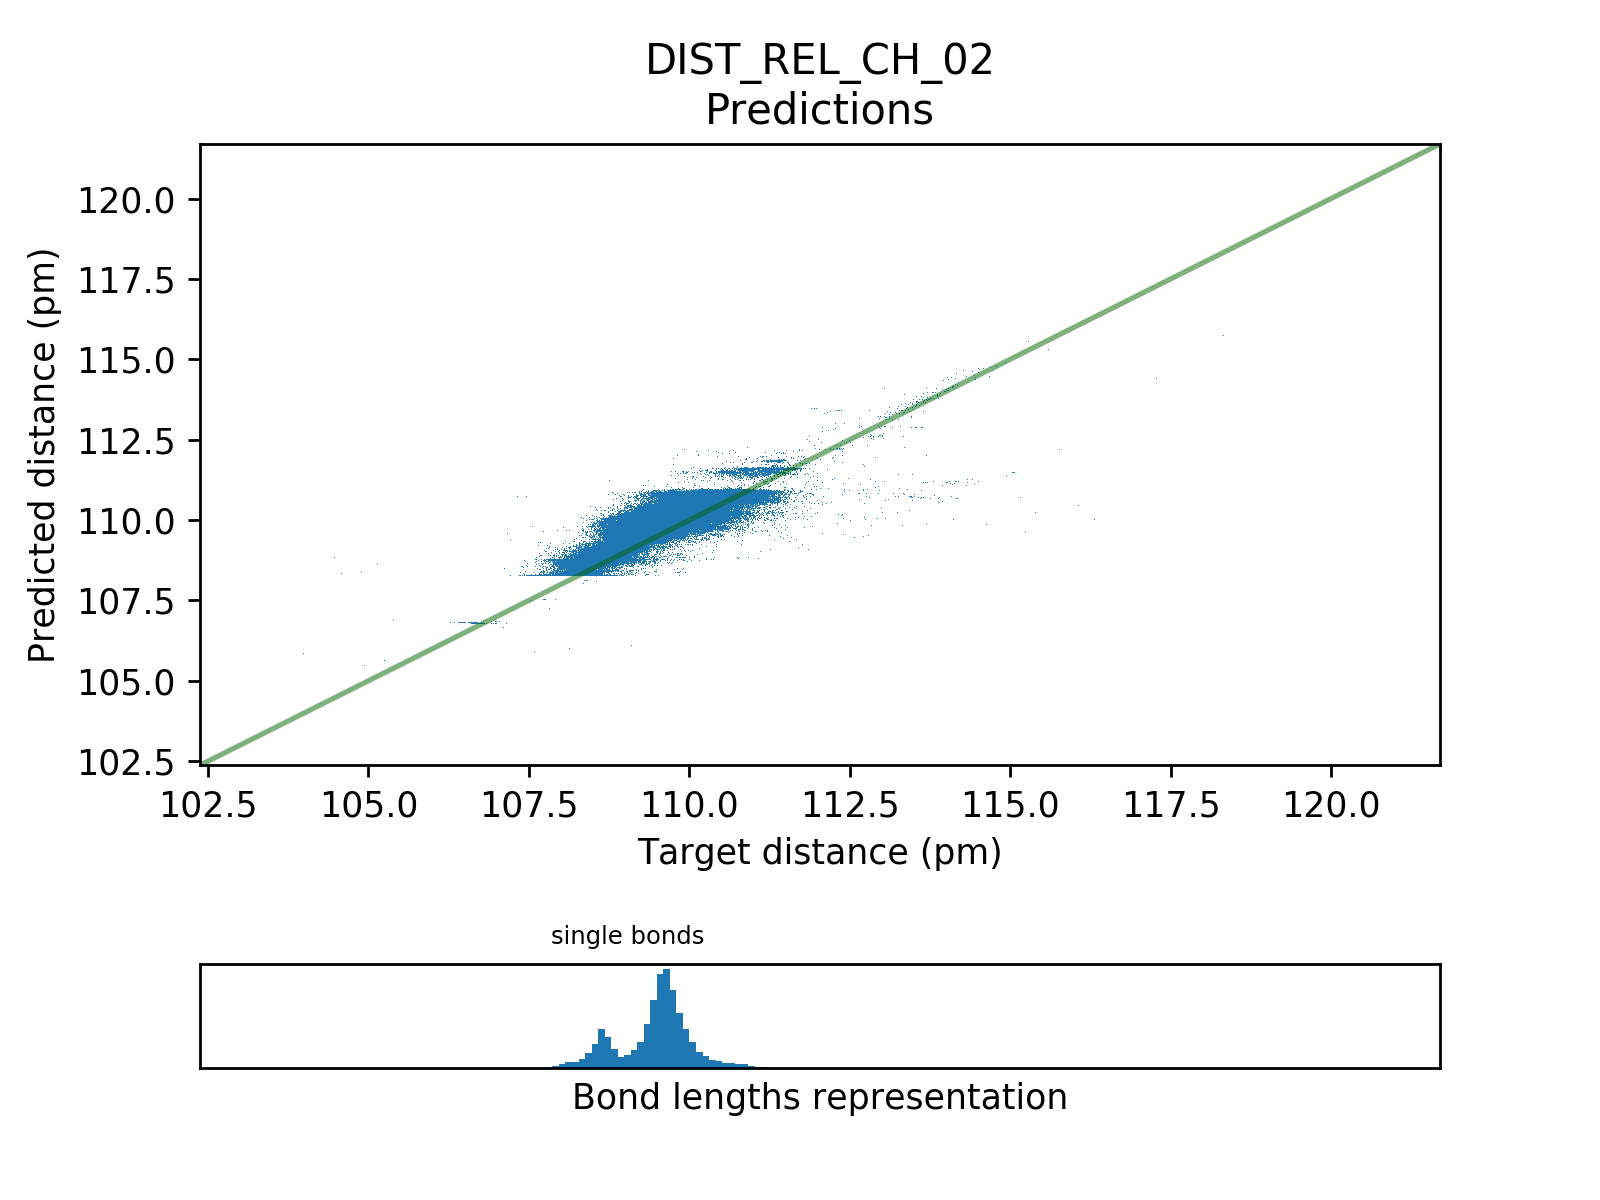
\includegraphics[scale=0.75]{../figures/DIST_REL_CH_02/DIST_REL_CH_02_preds_targets.png}	
	
	\caption{Prédictions en fonction des cibles pour le modèle \emph{DIST\_REL\_OH\_02}. Modèle s'entraînant sur une \textbf{grande quantité d'exemples} et prédisant les longueurs de liaisons \textbf{carbone-hydrogène}, à partir de données d'entrées sur lesquelles \textbf{aucune fonction} n'a été appliquée aux distances, \textbf{avec restriction} au voisinage le plus proche.}
	
\end{figure}


% DIST REL CC 03

\begin{figure}[!h]
	\centering
	
	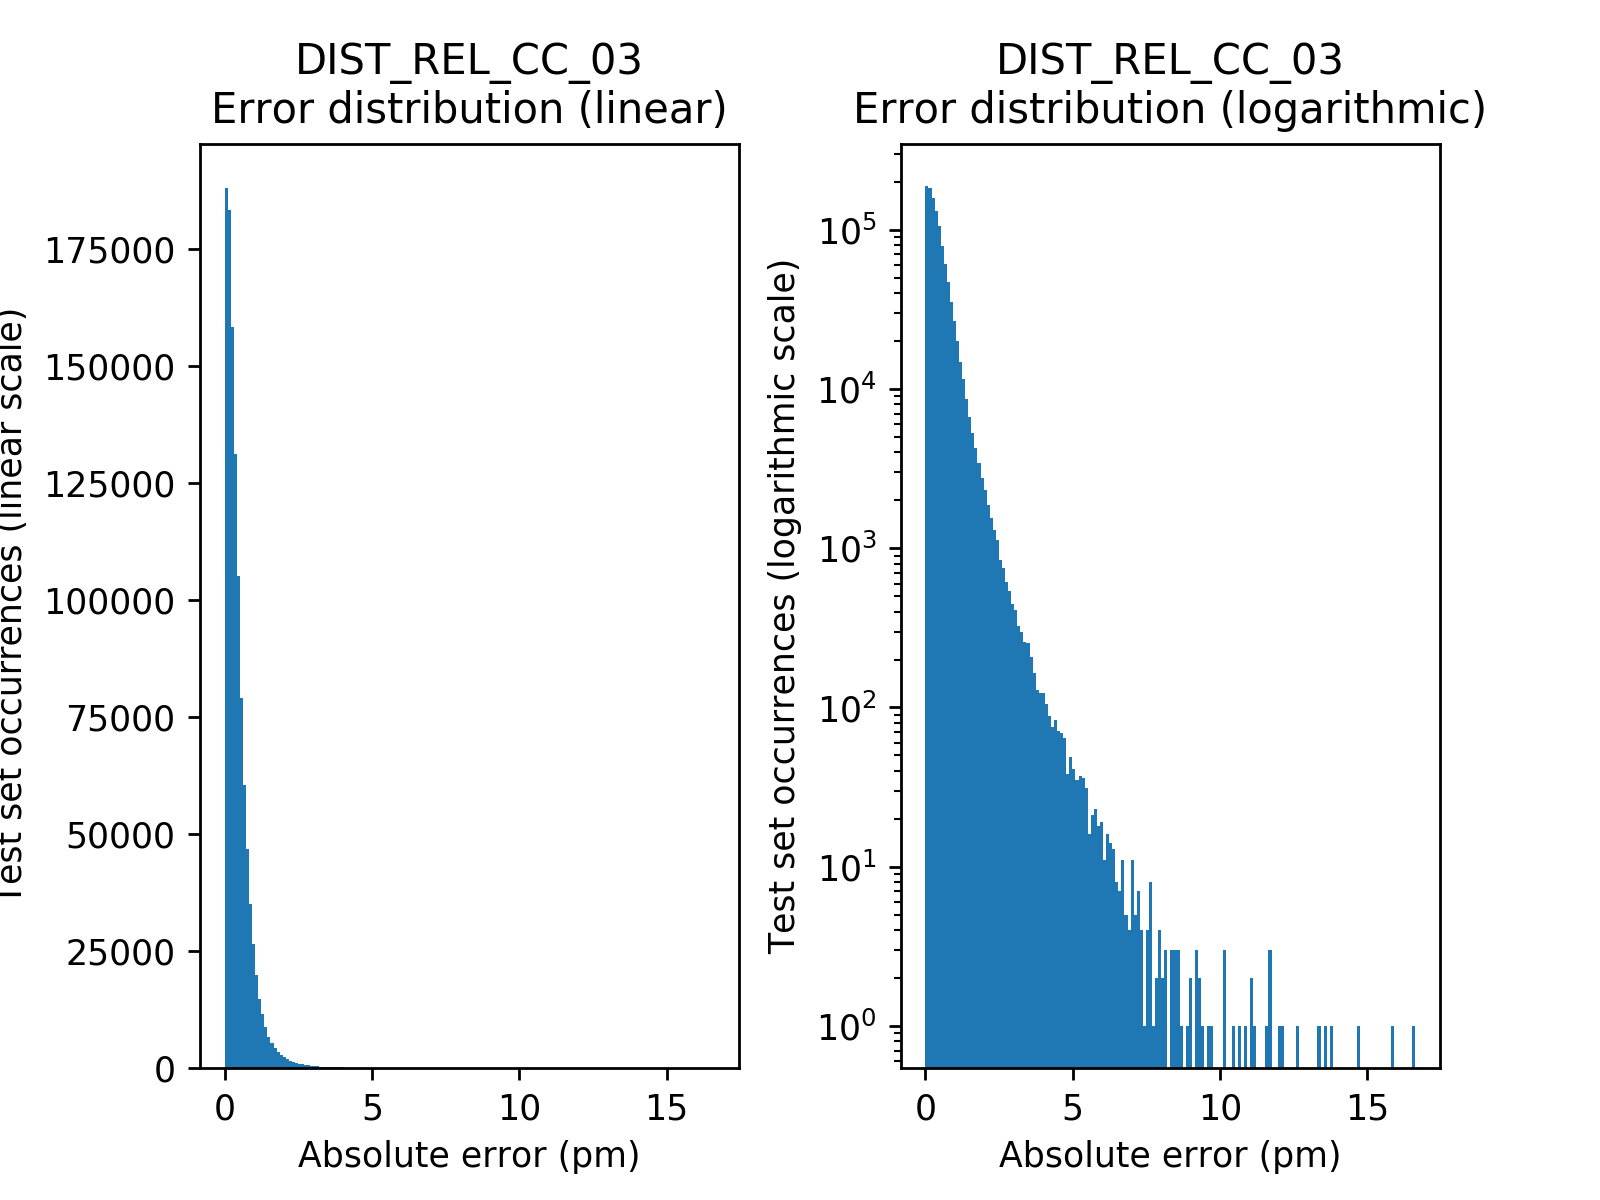
\includegraphics[scale=0.75]{../figures/DIST_REL_CC_03/DIST_REL_CC_03_distrib_rmse_val.png}	
	
	\caption{Distribution des erreurs du modèle \emph{DIST\_REL\_CC\_03}. Modèle s'entraînant sur une \textbf{grande quantité d'exemples} et prédisant les longueurs de liaisons \textbf{carbone-carbone}, à partir de données d'entrées sur lesquelles la \textbf{fonction inverse du carré} a été appliquée aux distances, \textbf{avec restriction} au voisinage le plus proche.}
\end{figure}

\begin{figure}[!h]
	\centering
	
	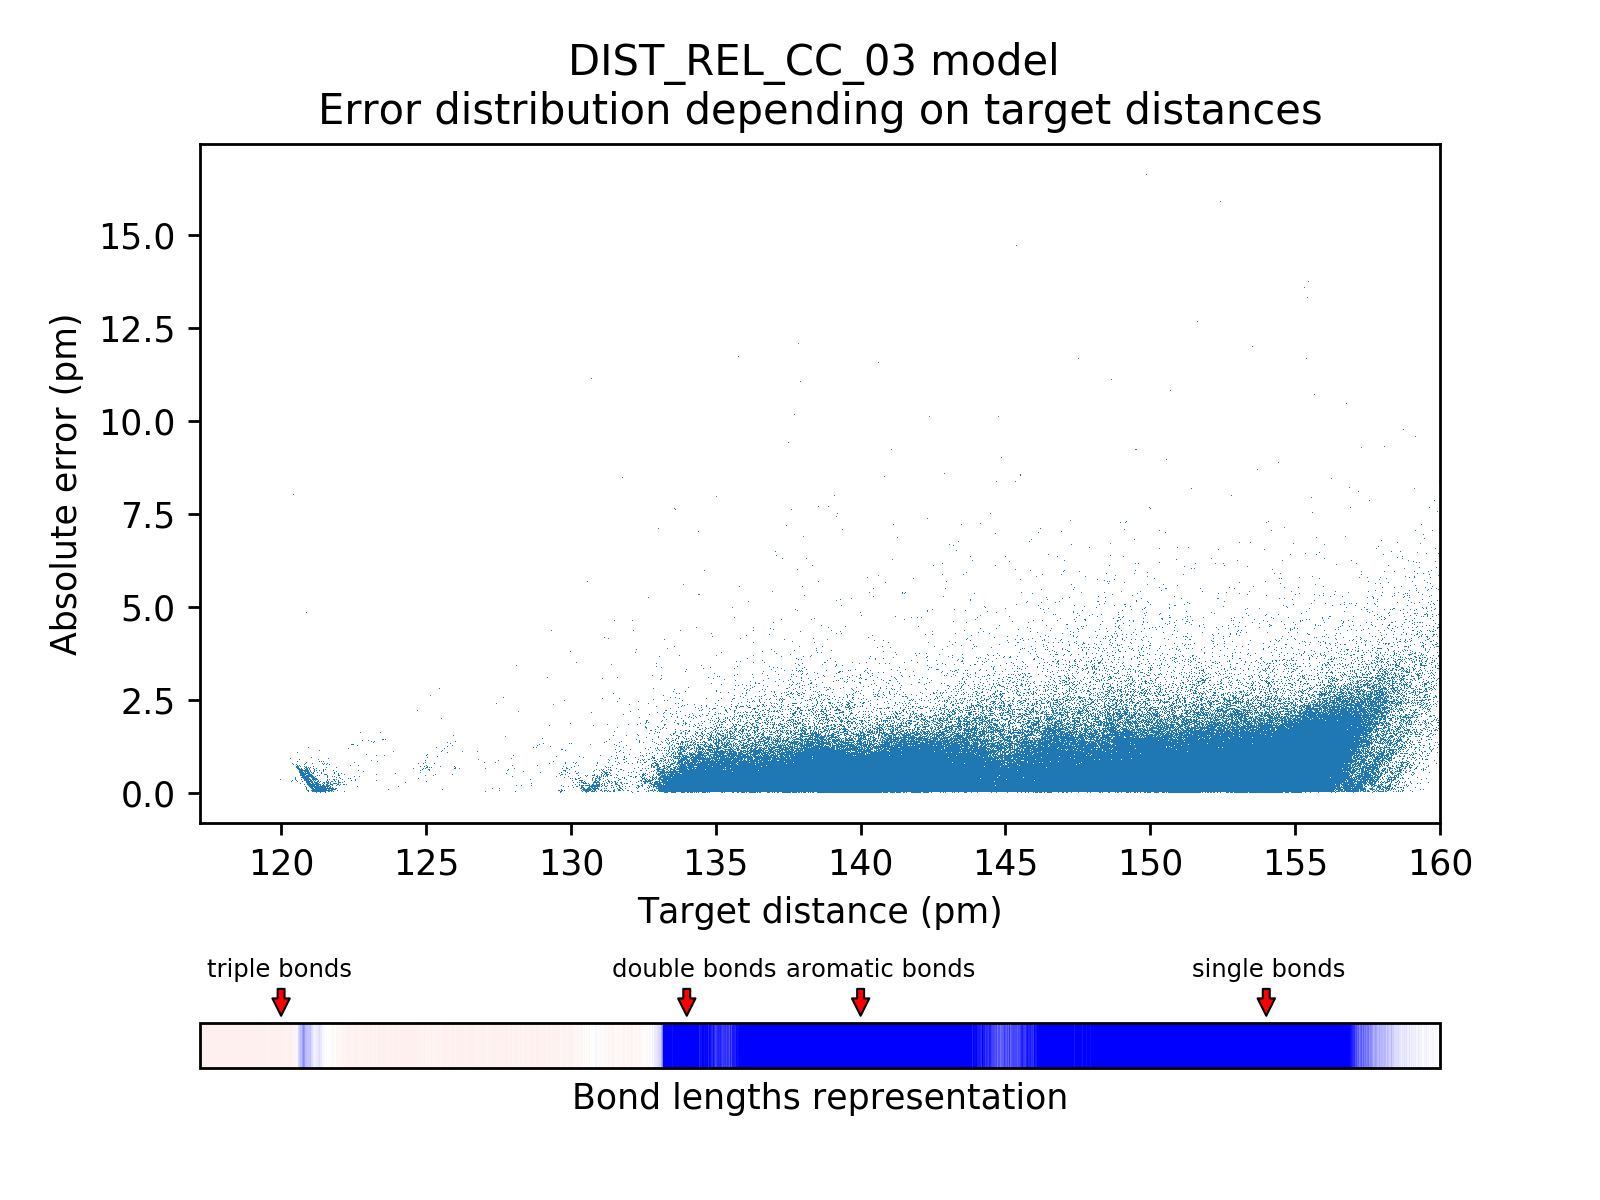
\includegraphics[scale=0.75]{../figures/DIST_REL_CC_03/DIST_REL_CC_03_distrib_rmse_dist.png}	
	
	\caption{Erreur en fonction des cibles pour le modèle \emph{DIST\_REL\_CC\_03}. Modèle s'entraînant sur une \textbf{grande quantité d'exemples} et prédisant les longueurs de liaisons \textbf{carbone-carbone}, à partir de données d'entrées sur lesquelles la \textbf{fonction inverse du carré} a été appliquée aux distances, \textbf{avec restriction} au voisinage le plus proche.}
\end{figure}

\begin{figure}[!h]
	\centering
	
	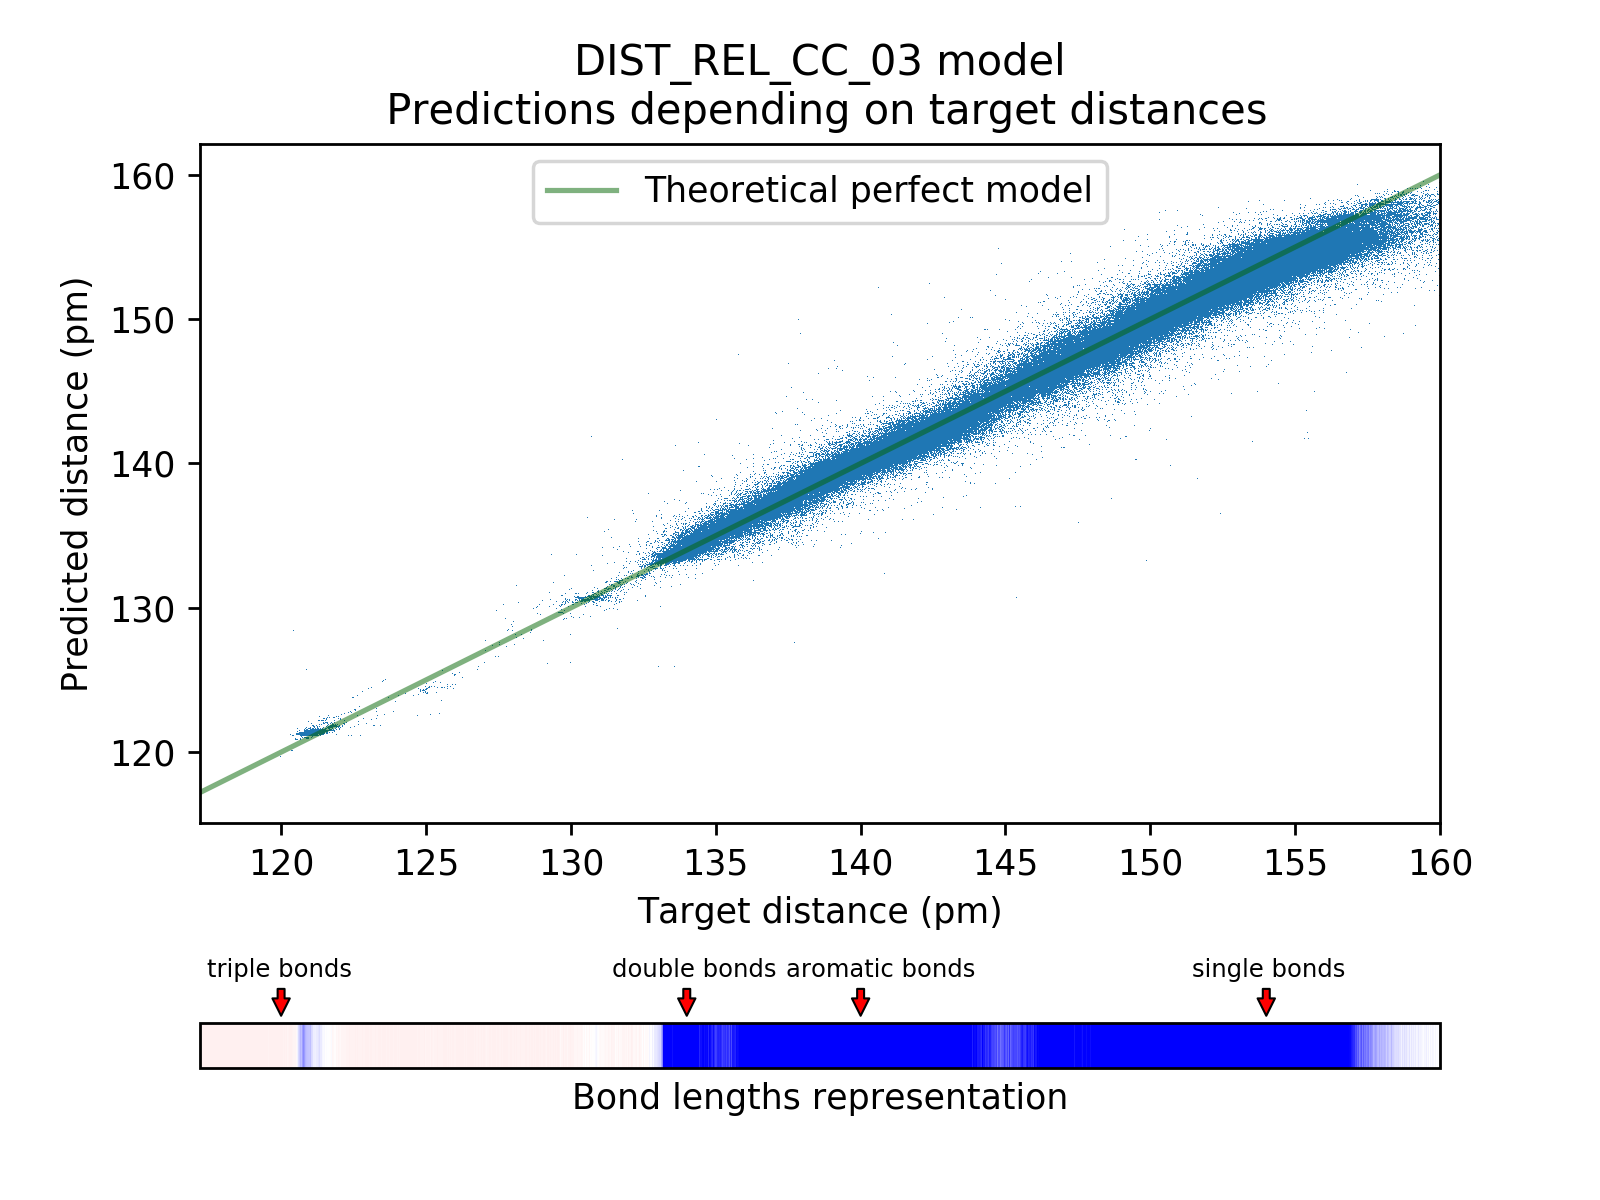
\includegraphics[scale=0.75]{../figures/DIST_REL_CC_03/DIST_REL_CC_03_preds_targets.png}	
	
	\caption{Prédictions en fonction des cibles pour le modèle \emph{DIST\_REL\_CC\_03}. Modèle s'entraînant sur une \textbf{grande quantité d'exemples} et prédisant les longueurs de liaisons \textbf{carbone-carbone}, à partir de données d'entrées sur lesquelles la \textbf{fonction inverse du carré} a été appliquée aux distances, \textbf{avec restriction} au voisinage le plus proche.}
	
\end{figure}

% DIST REL CH 03

\begin{figure}[!h]
	\centering
	
	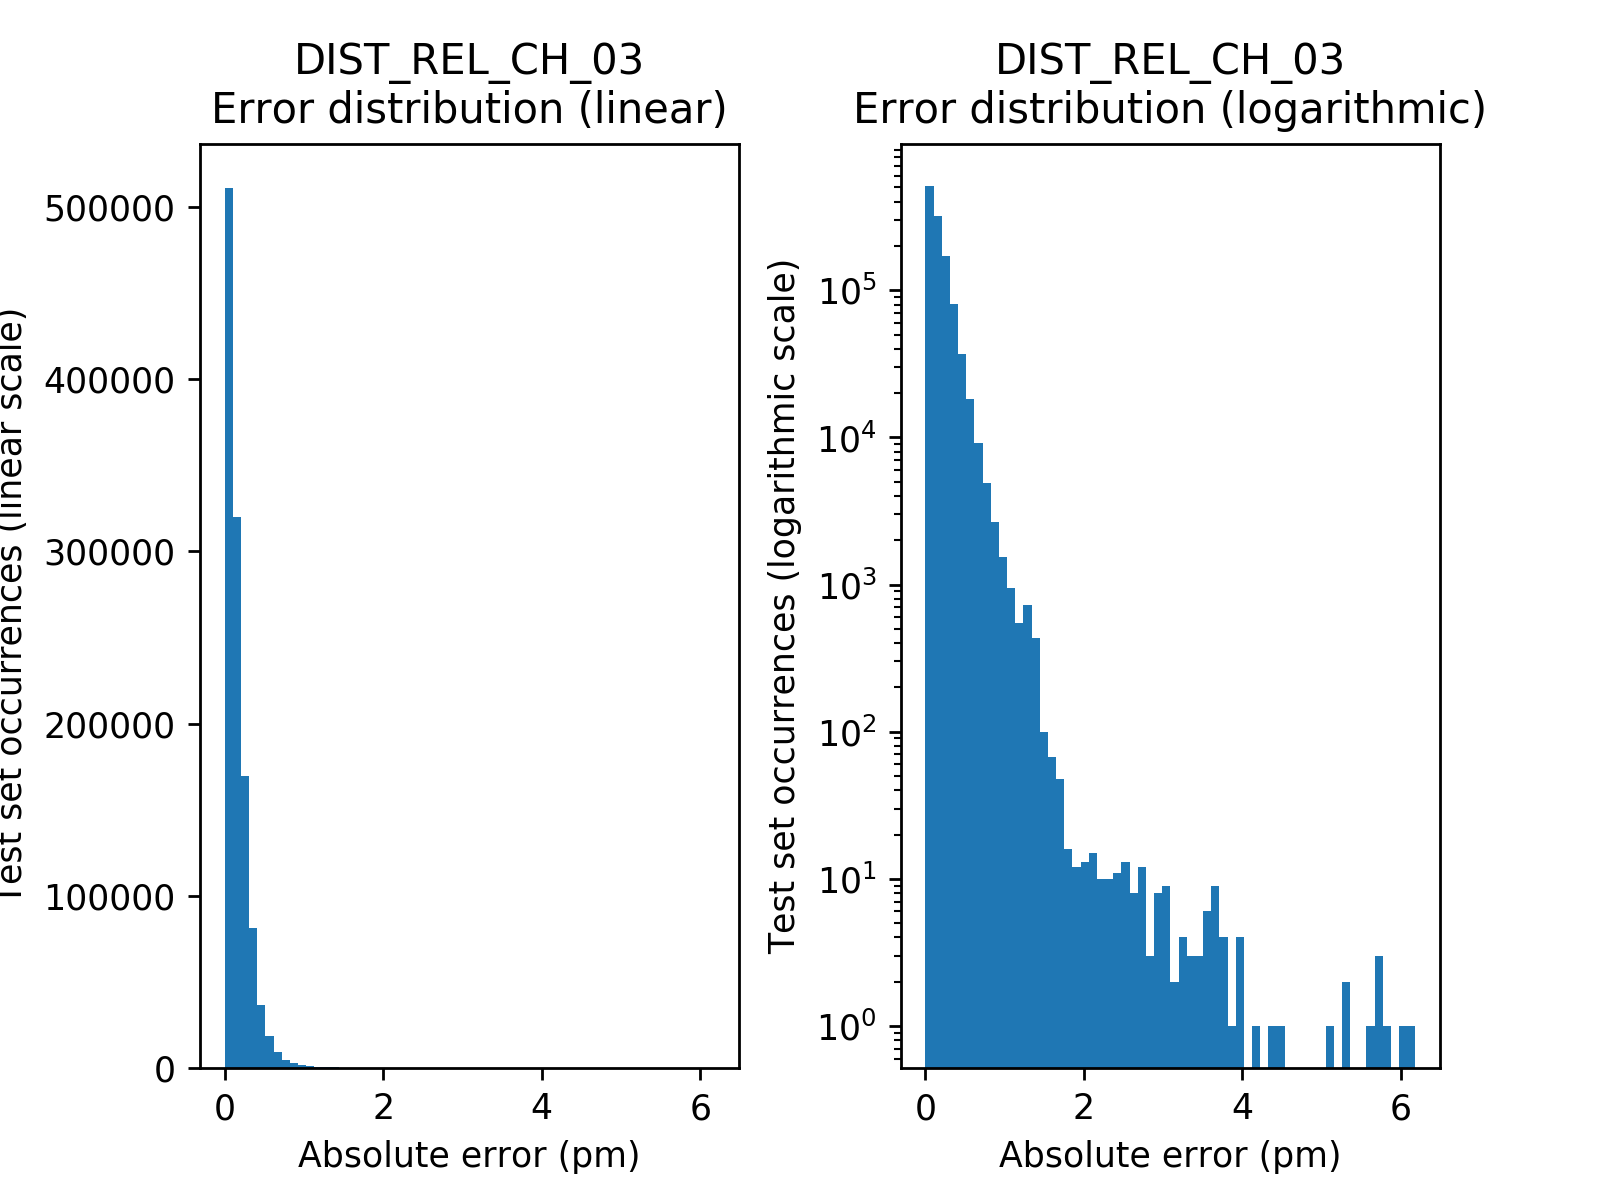
\includegraphics[scale=0.75]{../figures/DIST_REL_CH_03/DIST_REL_CH_03_distrib_rmse_val.png}	
	
	\caption{Distribution des erreurs du modèle \emph{DIST\_REL\_CH\_03}. Modèle s'entraînant sur une \textbf{grande quantité d'exemples} et prédisant les longueurs de liaisons \textbf{carbone-hydrogène}, à partir de données d'entrées sur lesquelles la \textbf{fonction inverse du carré} a été appliquée aux distances, \textbf{avec restriction} au voisinage le plus proche.}
\end{figure}

\begin{figure}[!h]
	\centering
	
	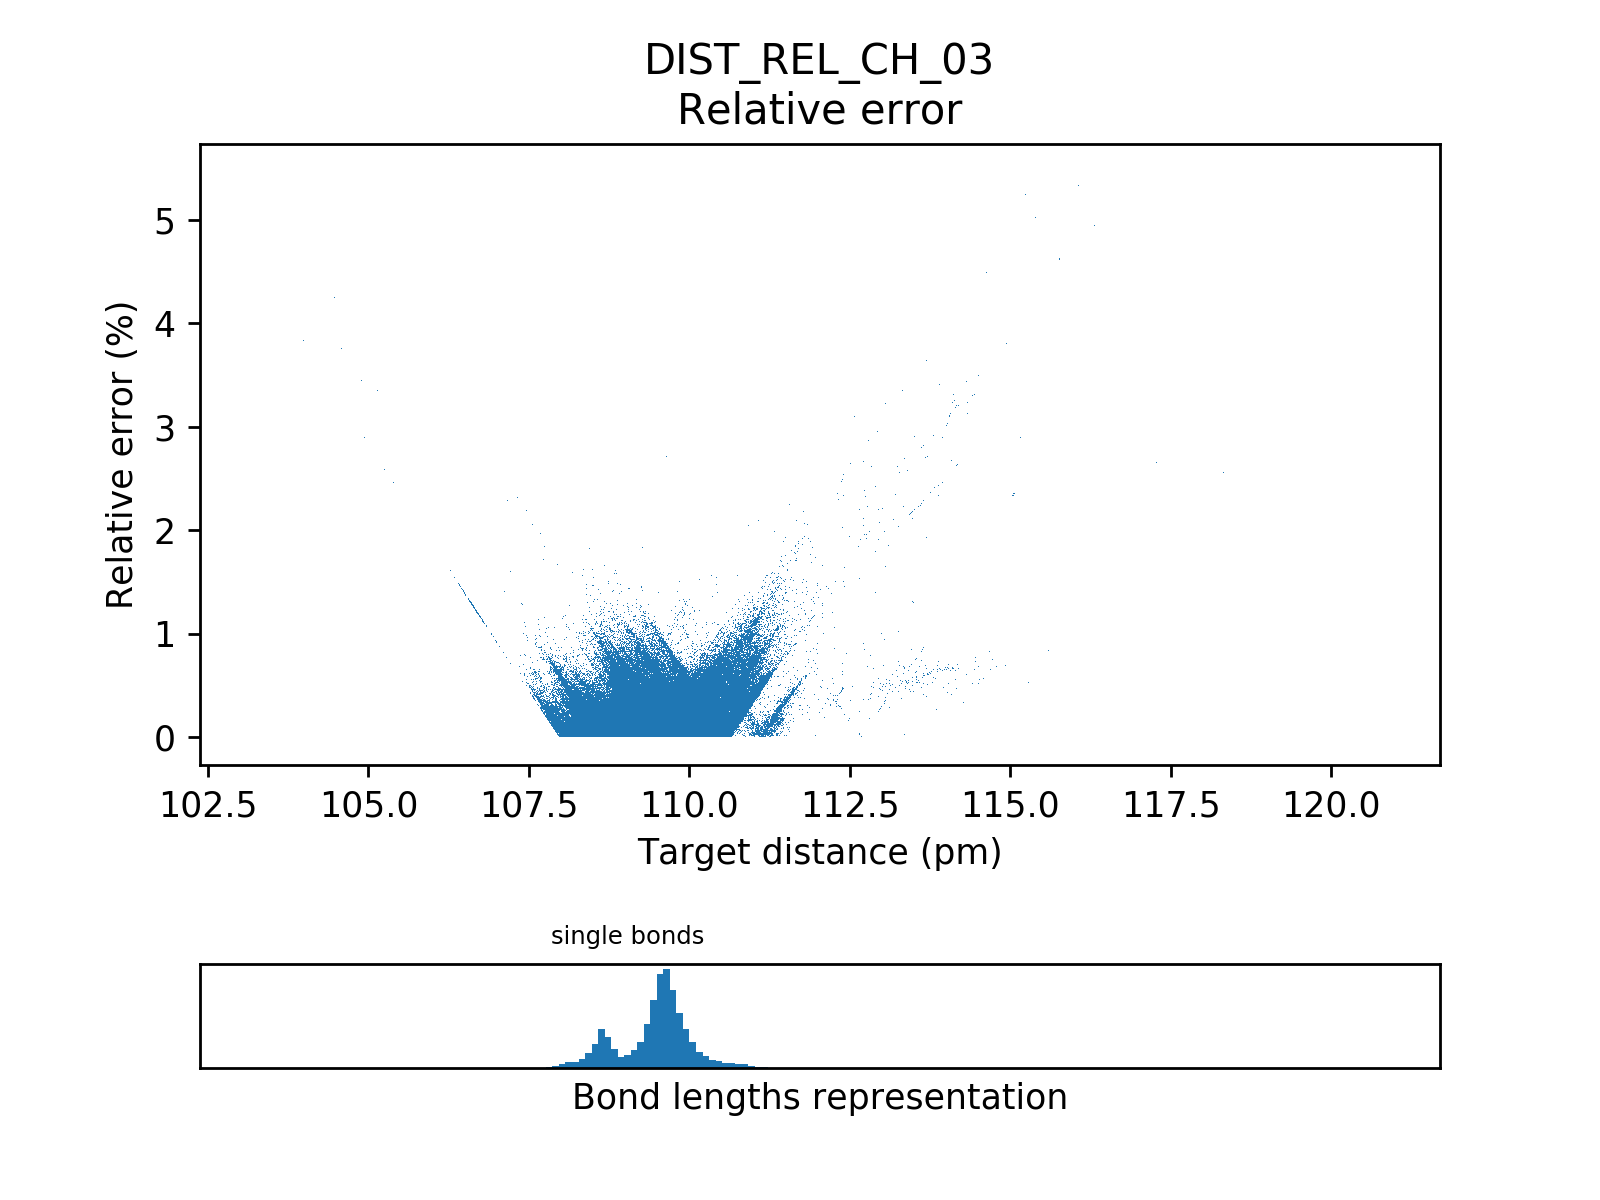
\includegraphics[scale=0.75]{../figures/DIST_REL_CH_03/DIST_REL_CH_03_distrib_rmse_dist.png}	
	
	\caption{Erreur en fonction des cibles pour le modèle \emph{DIST\_REL\_CH\_03}. Modèle s'entraînant sur une \textbf{grande quantité d'exemples} et prédisant les longueurs de liaisons \textbf{carbone-hydrogène}, à partir de données d'entrées sur lesquelles la \textbf{fonction inverse du carré} a été appliquée aux distances, \textbf{avec restriction} au voisinage le plus proche.}
\end{figure}

\begin{figure}[!h]
	\centering
	
	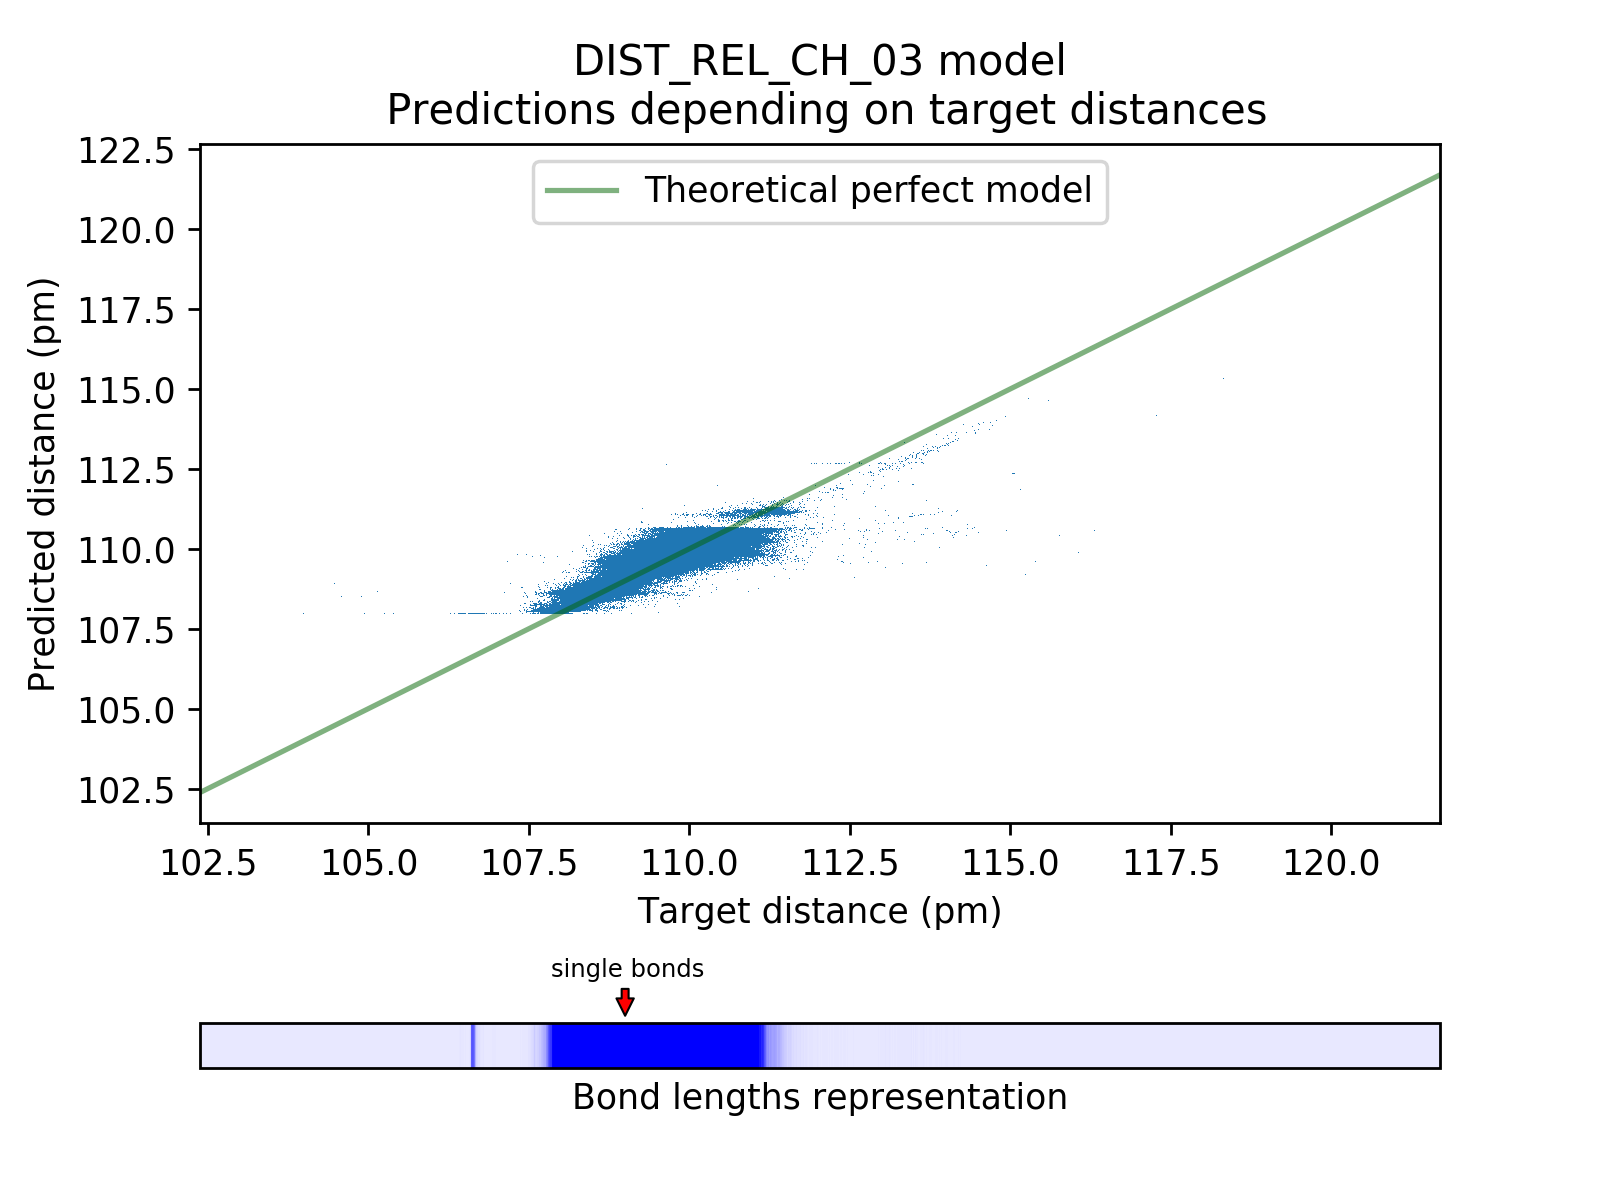
\includegraphics[scale=0.75]{../figures/DIST_REL_CH_03/DIST_REL_CH_03_preds_targets.png}	
	
	\caption{Prédictions en fonction des cibles pour le modèle \emph{DIST\_REL\_CH\_03}. Modèle s'entraînant sur une \textbf{grande quantité d'exemples} et prédisant les longueurs de liaisons \textbf{carbone-hydrogène}, à partir de données d'entrées sur lesquelles la \textbf{fonction inverse du carré} a été appliquée aux distances, \textbf{avec restriction} au voisinage le plus proche.}
	
\end{figure}

% DIST REL OH 03

\begin{figure}[!h]
	\centering
	
	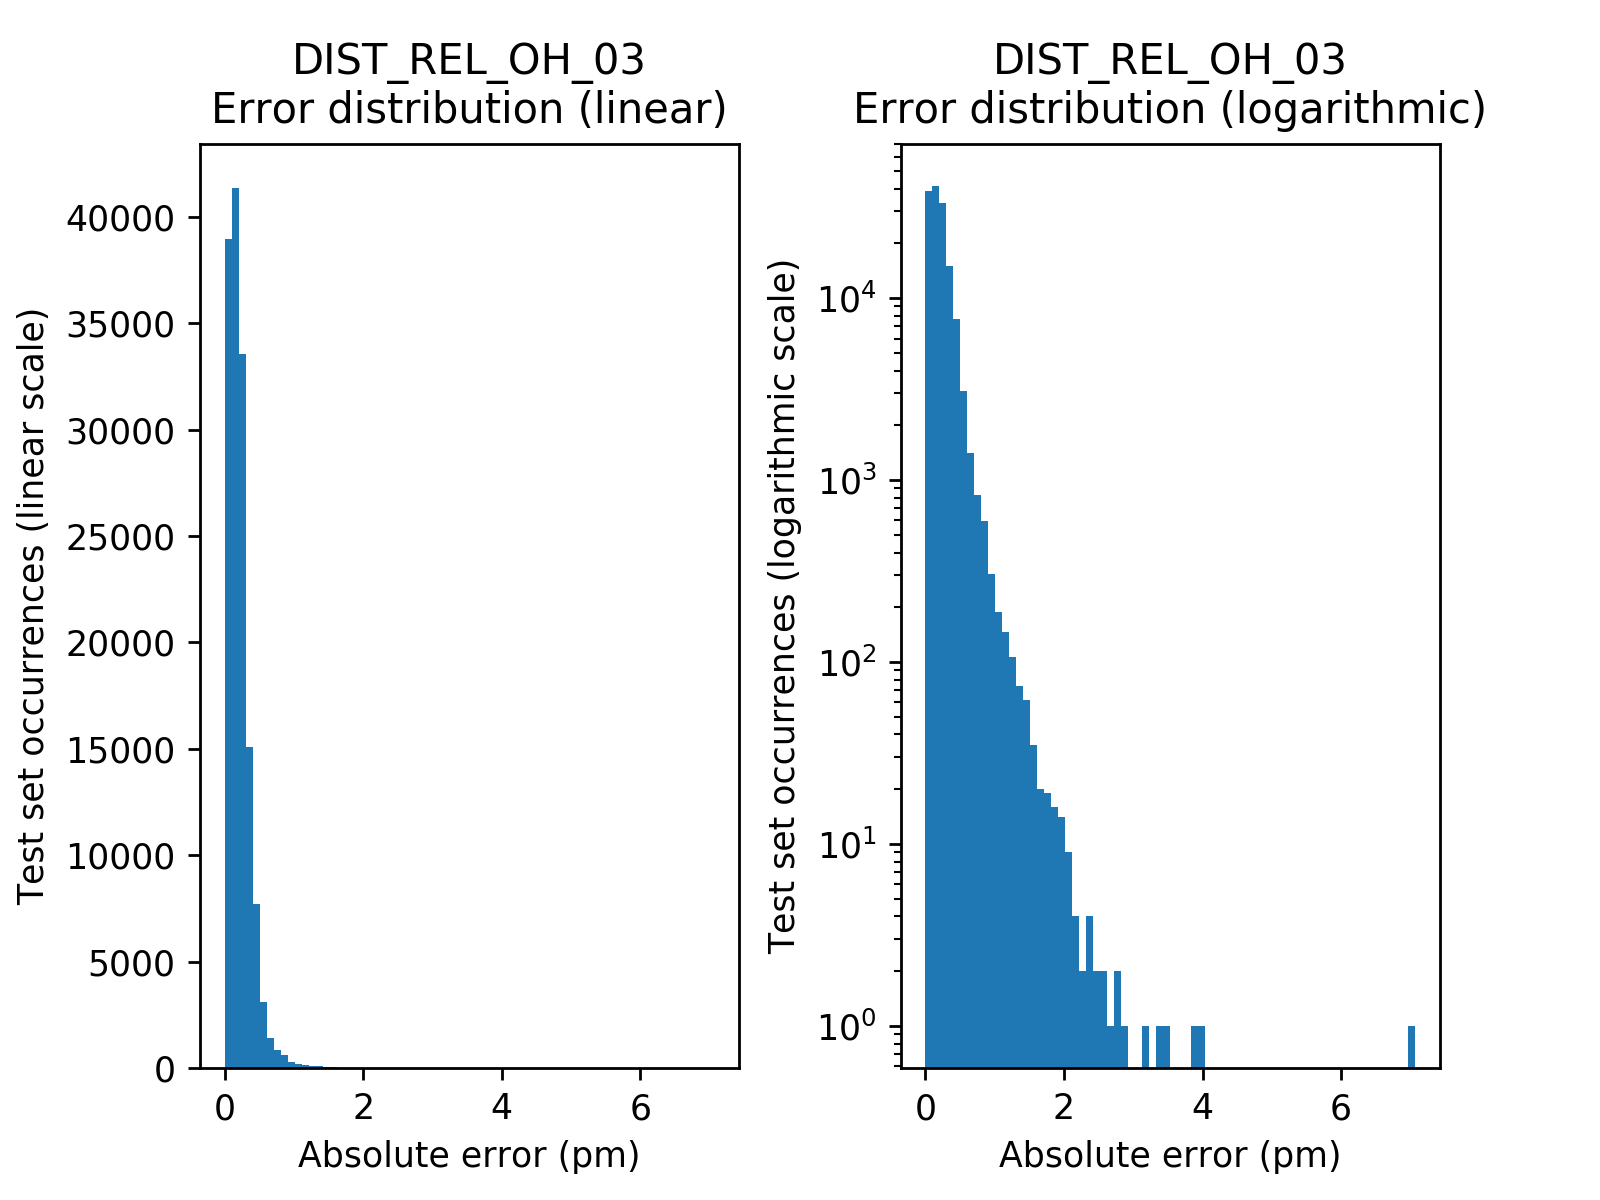
\includegraphics[scale=0.75]{../figures/DIST_REL_OH_03/DIST_REL_OH_03_distrib_rmse_val.png}	
	
	\caption{Distribution des erreurs du modèle \emph{DIST\_REL\_OH\_03}. Modèle s'entraînant sur une \textbf{grande quantité d'exemples} et prédisant les longueurs de liaisons \textbf{oxygène-hydrogène}, à partir de données d'entrées sur lesquelles la \textbf{fonction inverse du carré} a été appliquée aux distances, \textbf{avec restriction} au voisinage le plus proche.}
\end{figure}

\begin{figure}[!h]
	\centering
	
	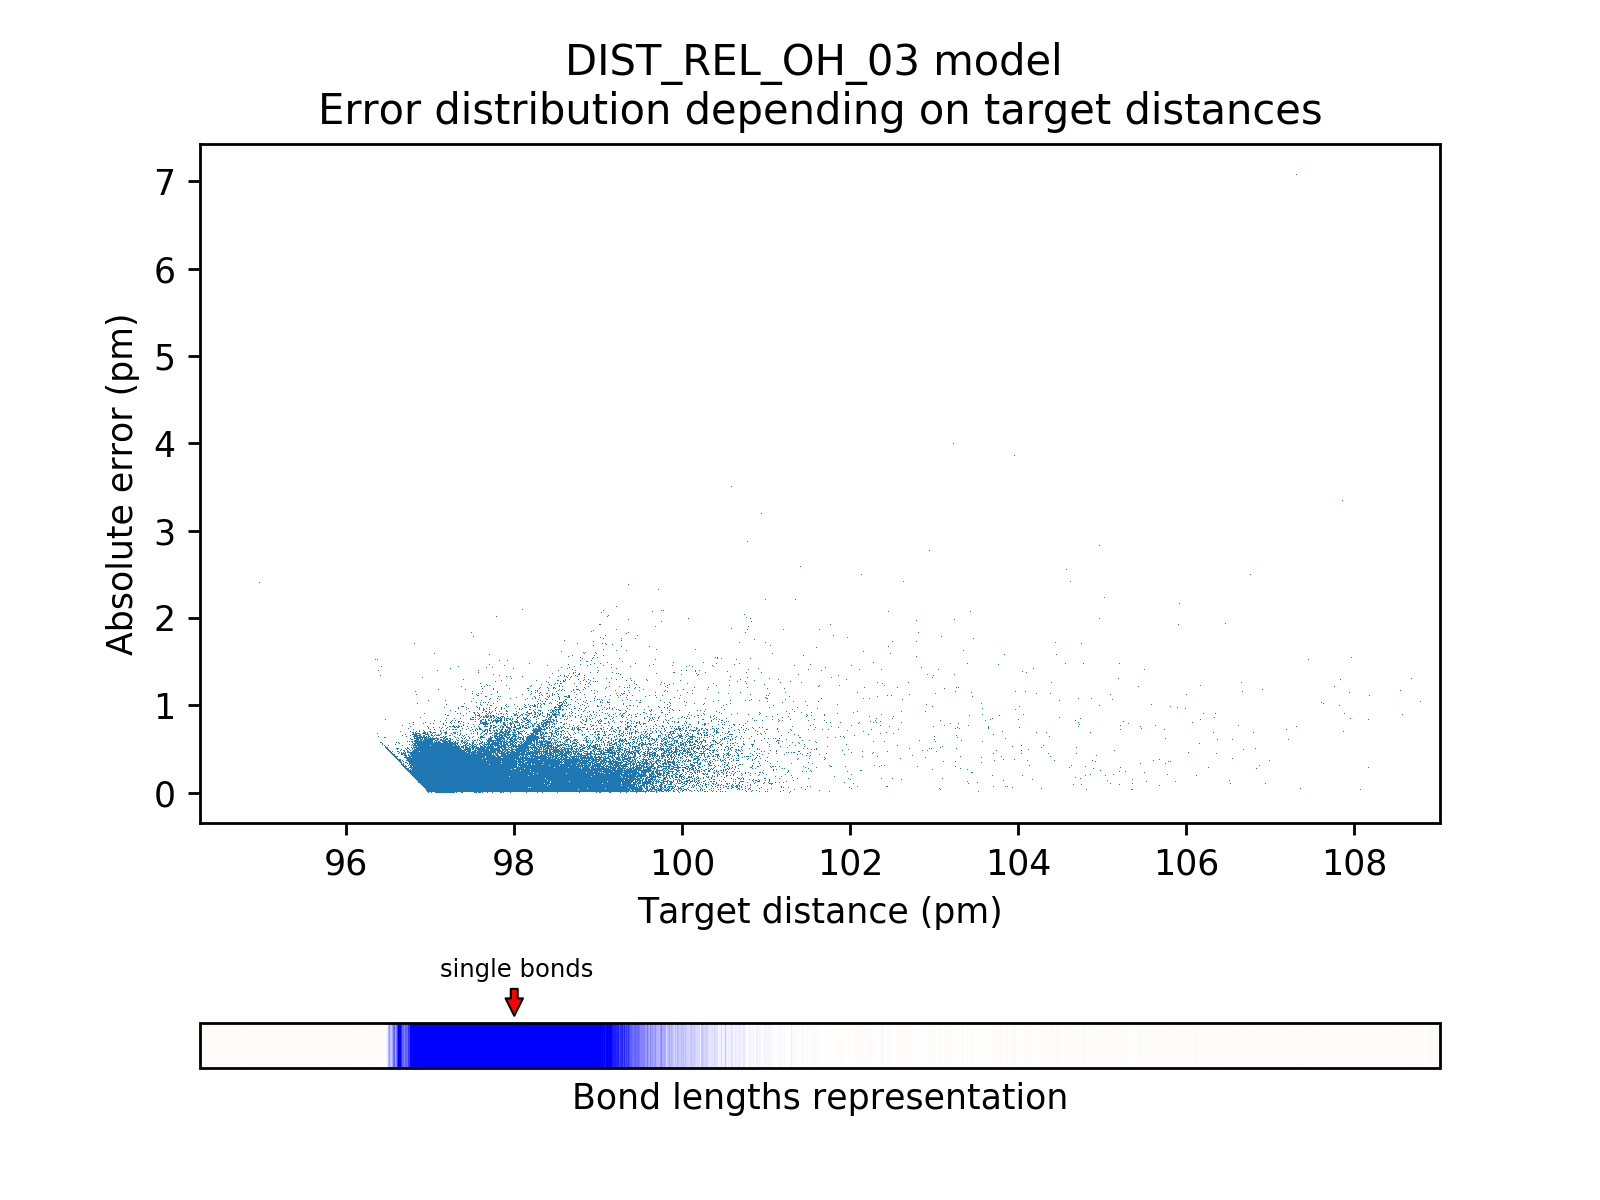
\includegraphics[scale=0.75]{../figures/DIST_REL_OH_03/DIST_REL_OH_03_distrib_rmse_dist.png}	
	
	\caption{Erreur en fonction des cibles pour le modèle \emph{DIST\_REL\_OH\_03}. Modèle s'entraînant sur une \textbf{grande quantité d'exemples} et prédisant les longueurs de liaisons \textbf{oxygène-hydrogène}, à partir de données d'entrées sur lesquelles la \textbf{fonction inverse du carré} a été appliquée aux distances, \textbf{avec restriction} au voisinage le plus proche.}
\end{figure}

\begin{figure}[!h]
	\centering
	
	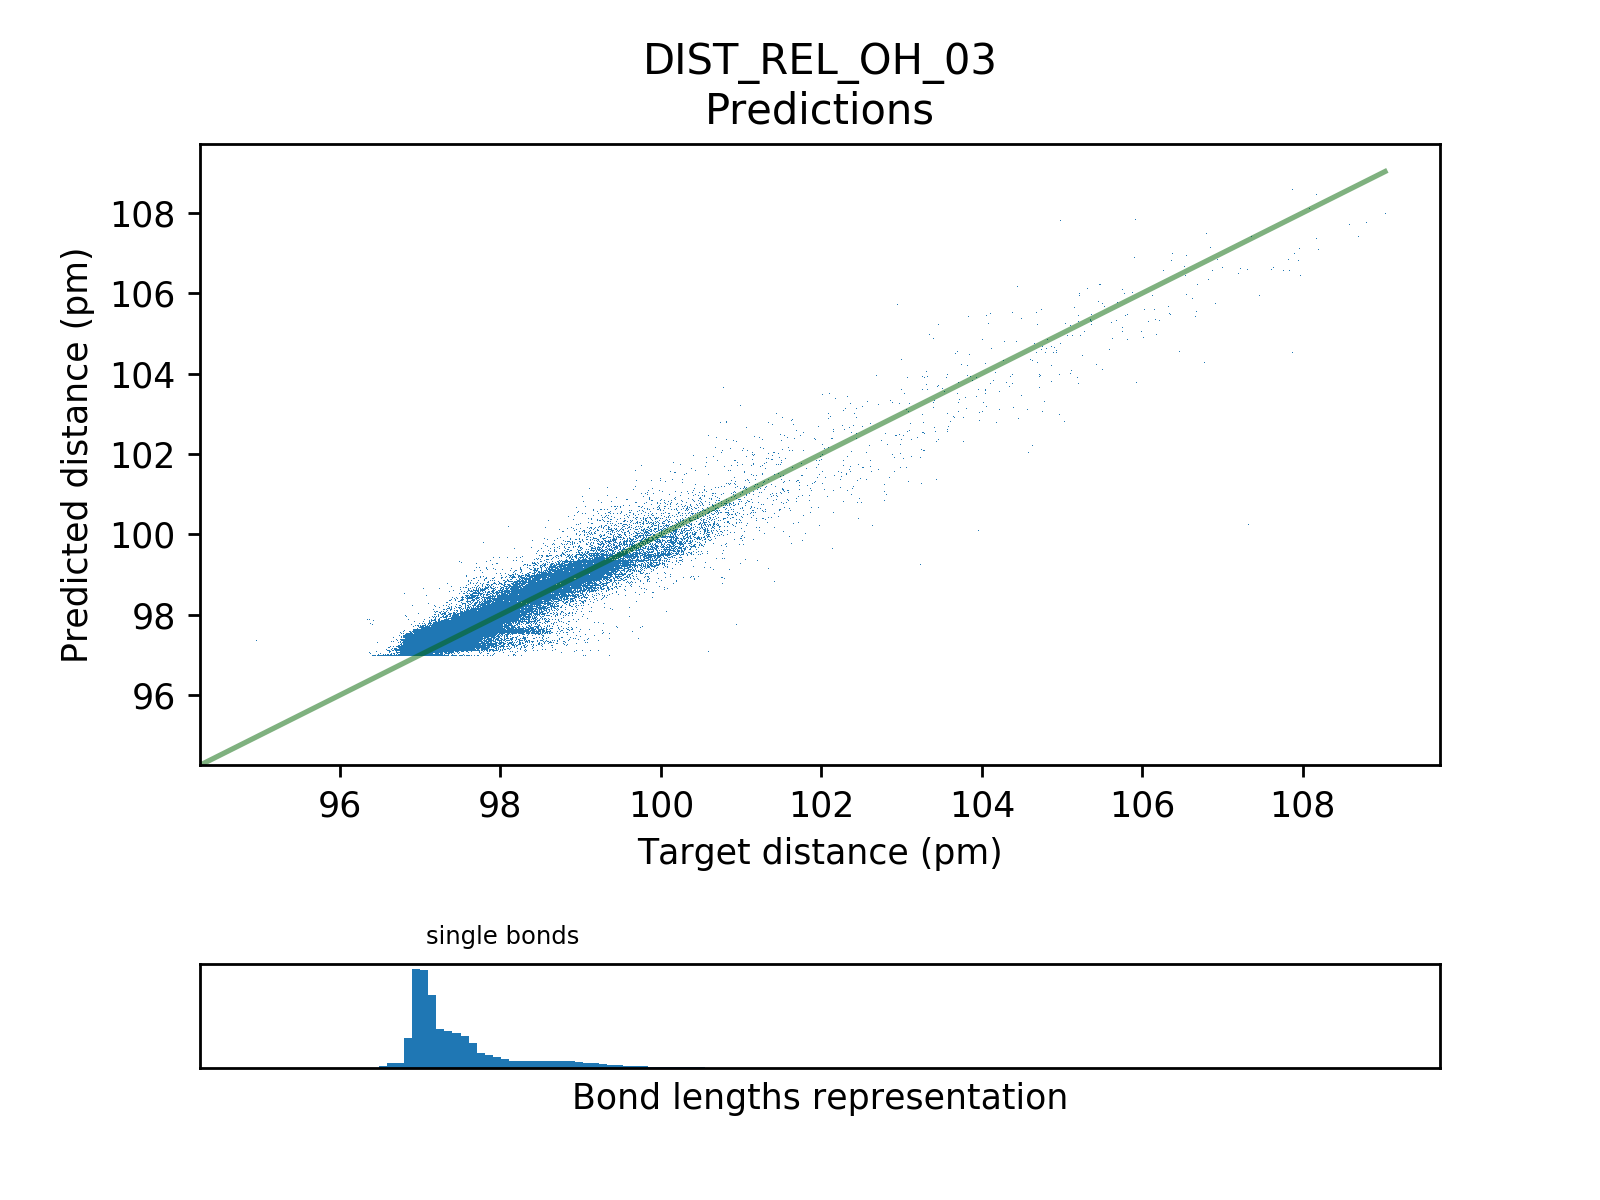
\includegraphics[scale=0.75]{../figures/DIST_REL_OH_03/DIST_REL_OH_03_preds_targets.png}	
	
	\caption{Prédictions en fonction des cibles pour le modèle \emph{DIST\_REL\_OH\_03}. Modèle s'entraînant sur une \textbf{grande quantité d'exemples} et prédisant les longueurs de liaisons \textbf{oxygène-hydrogène}, à partir de données d'entrées sur lesquelles la \textbf{fonction inverse du carré} a été appliquée aux distances, \textbf{avec restriction} au voisinage le plus proche.}
	
\end{figure}


% DIST REL CC 04

\begin{figure}[!h]
	\centering
	
	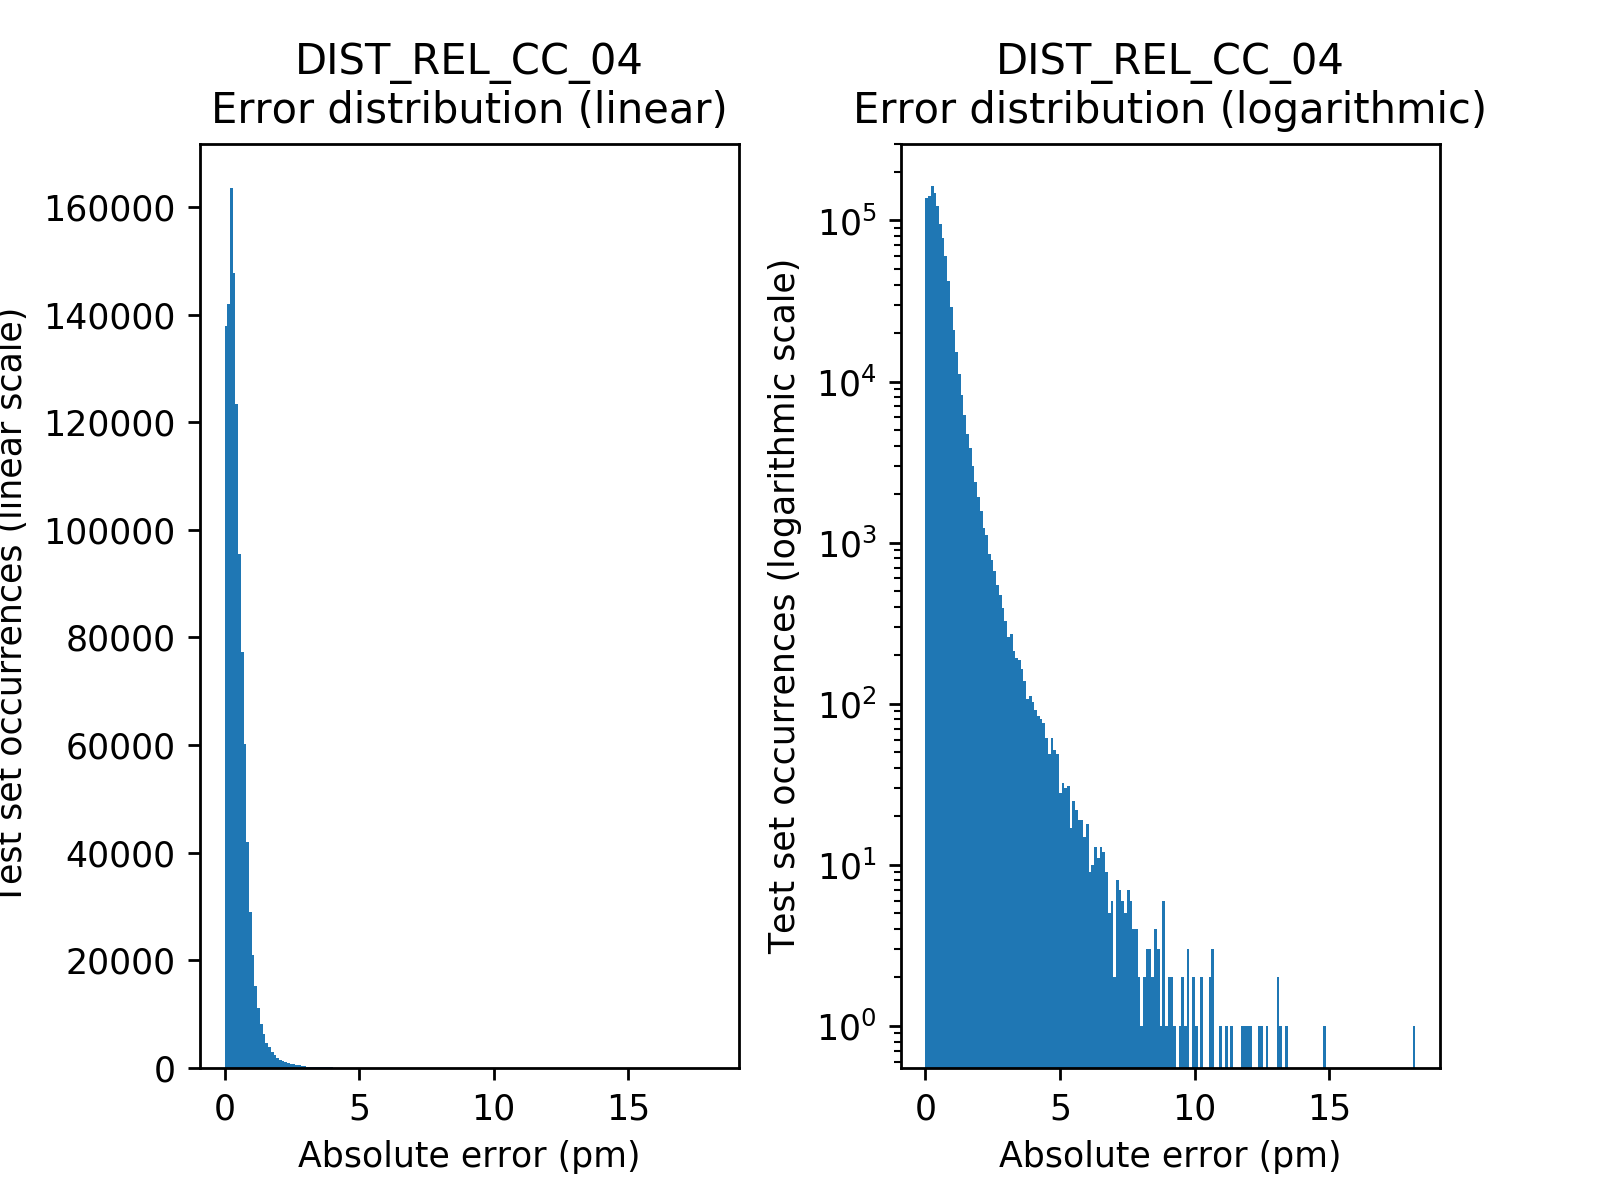
\includegraphics[scale=0.75]{../figures/DIST_REL_CC_04/DIST_REL_CC_04_distrib_rmse_val.png}	
	
	\caption{Distribution des erreurs du modèle \emph{DIST\_REL\_CC\_04}. Modèle s'entraînant sur une \textbf{grande quantité d'exemples} et prédisant les longueurs de liaisons \textbf{carbone-carbone}, à partir de données d'entrées sur lesquelles la \textbf{fonction inverse} a été appliquée aux distances, \textbf{avec restriction} au voisinage le plus proche.}
\end{figure}

\begin{figure}[!h]
	\centering
	
	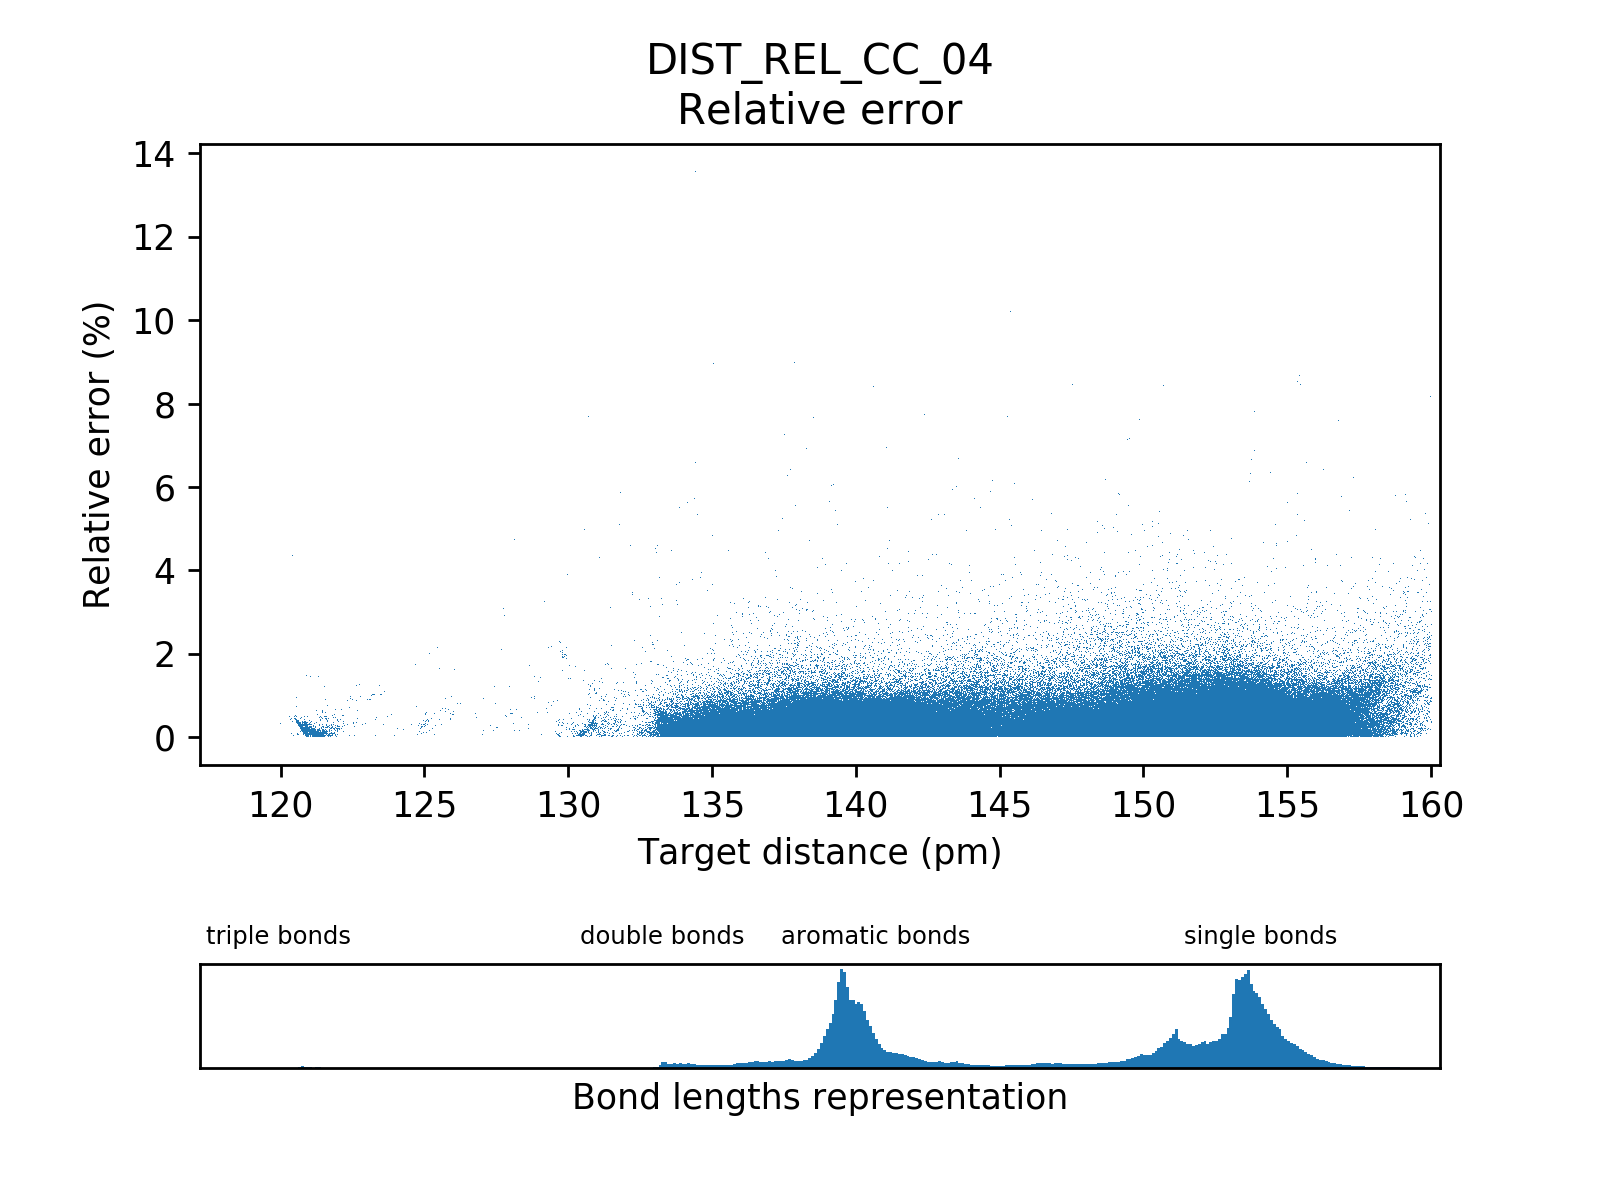
\includegraphics[scale=0.75]{../figures/DIST_REL_CC_04/DIST_REL_CC_04_distrib_rmse_dist.png}	
	
	\caption{Erreur en fonction des cibles pour le modèle \emph{DIST\_REL\_CC\_04}. Modèle s'entraînant sur une \textbf{grande quantité d'exemples} et prédisant les longueurs de liaisons \textbf{carbone-carbone}, à partir de données d'entrées sur lesquelles la \textbf{fonction inverse} a été appliquée aux distances, \textbf{avec restriction} au voisinage le plus proche.}
\end{figure}

\begin{figure}[!h]
	\centering
	
	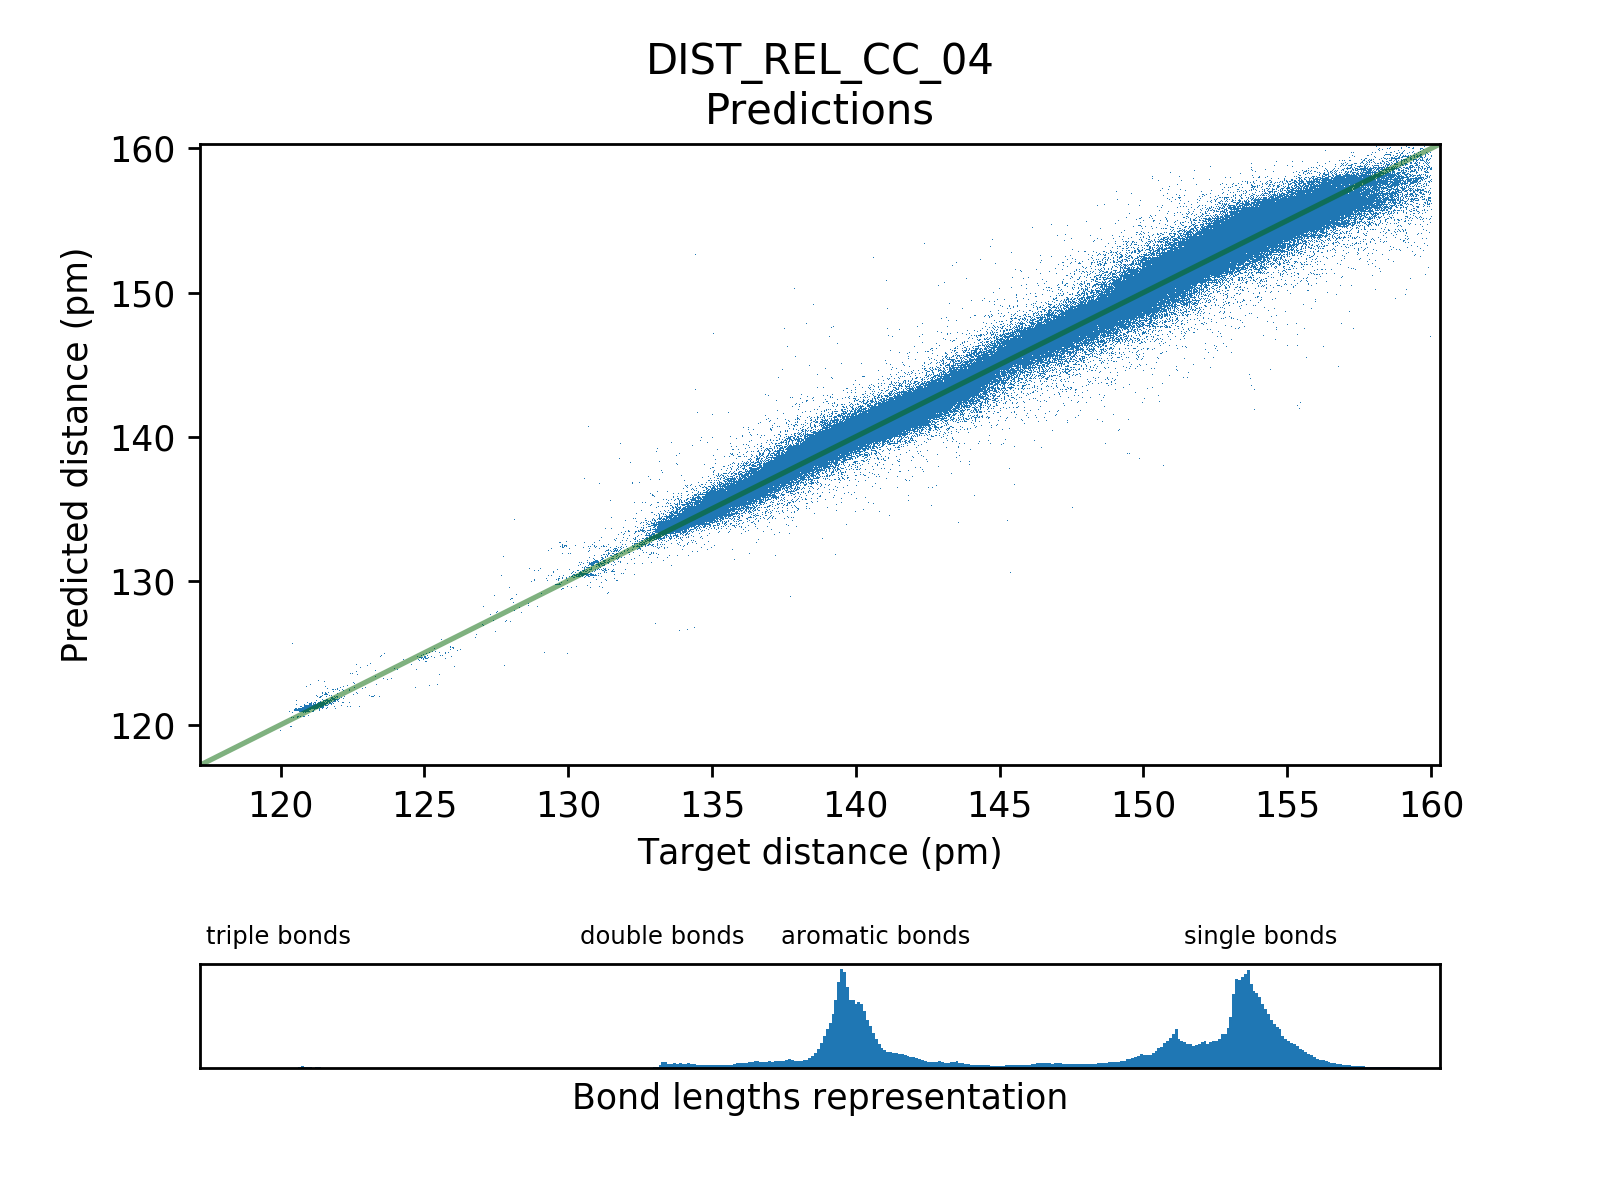
\includegraphics[scale=0.75]{../figures/DIST_REL_CC_04/DIST_REL_CC_04_preds_targets.png}	
	
	\caption{Prédictions en fonction des cibles pour le modèle \emph{DIST\_REL\_CC\_04}. Modèle s'entraînant sur une \textbf{grande quantité d'exemples} et prédisant les longueurs de liaisons \textbf{carbone-carbone}, à partir de données d'entrées sur lesquelles la \textbf{fonction inverse} a été appliquée aux distances, \textbf{avec restriction} au voisinage le plus proche.}
	
\end{figure}

% DIST REL CH 04

\begin{figure}[!h]
	\centering
	
	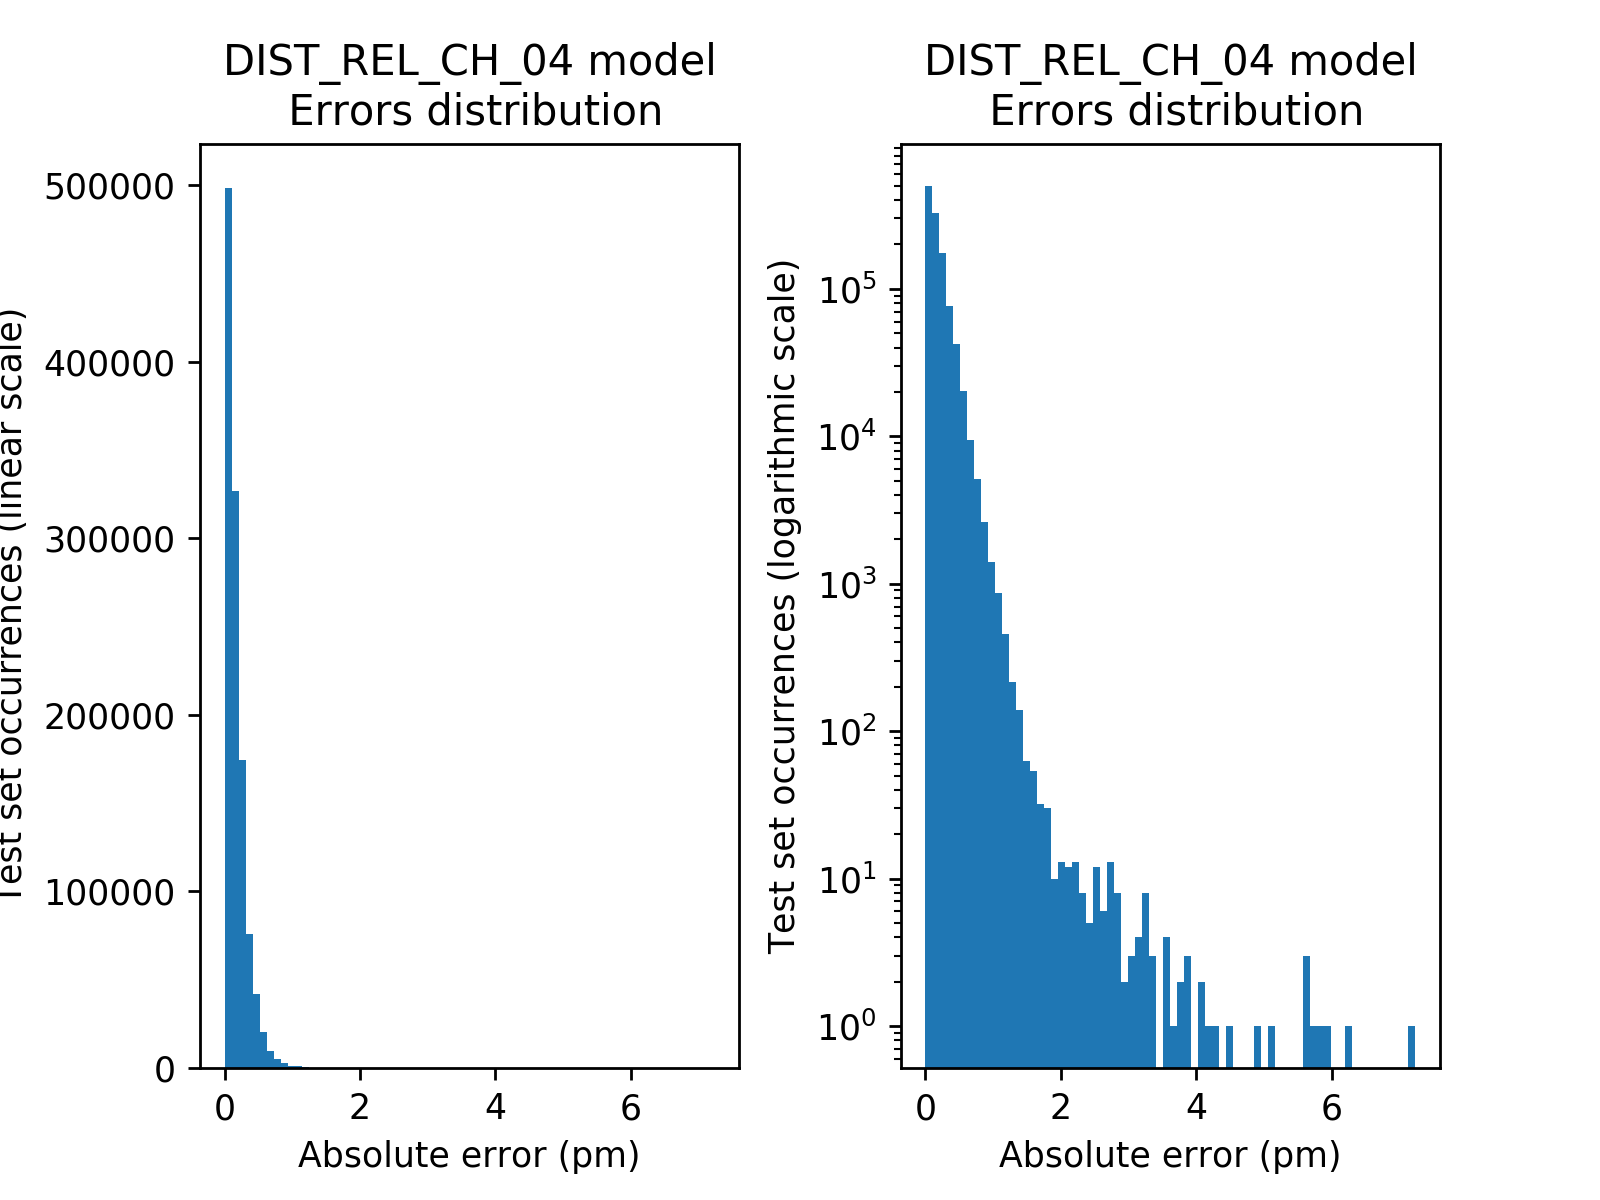
\includegraphics[scale=0.75]{../figures/DIST_REL_CH_04/DIST_REL_CH_04_distrib_rmse_val.png}	
	
	\caption{Distribution des erreurs du modèle \emph{DIST\_REL\_CH\_04}. Modèle s'entraînant sur une \textbf{grande quantité d'exemples} et prédisant les longueurs de liaisons \textbf{carbone-hydrogene}, à partir de données d'entrées sur lesquelles la \textbf{fonction inverse} a été appliquée aux distances, \textbf{avec restriction} au voisinage le plus proche.}
\end{figure}

\begin{figure}[!h]
	\centering
	
	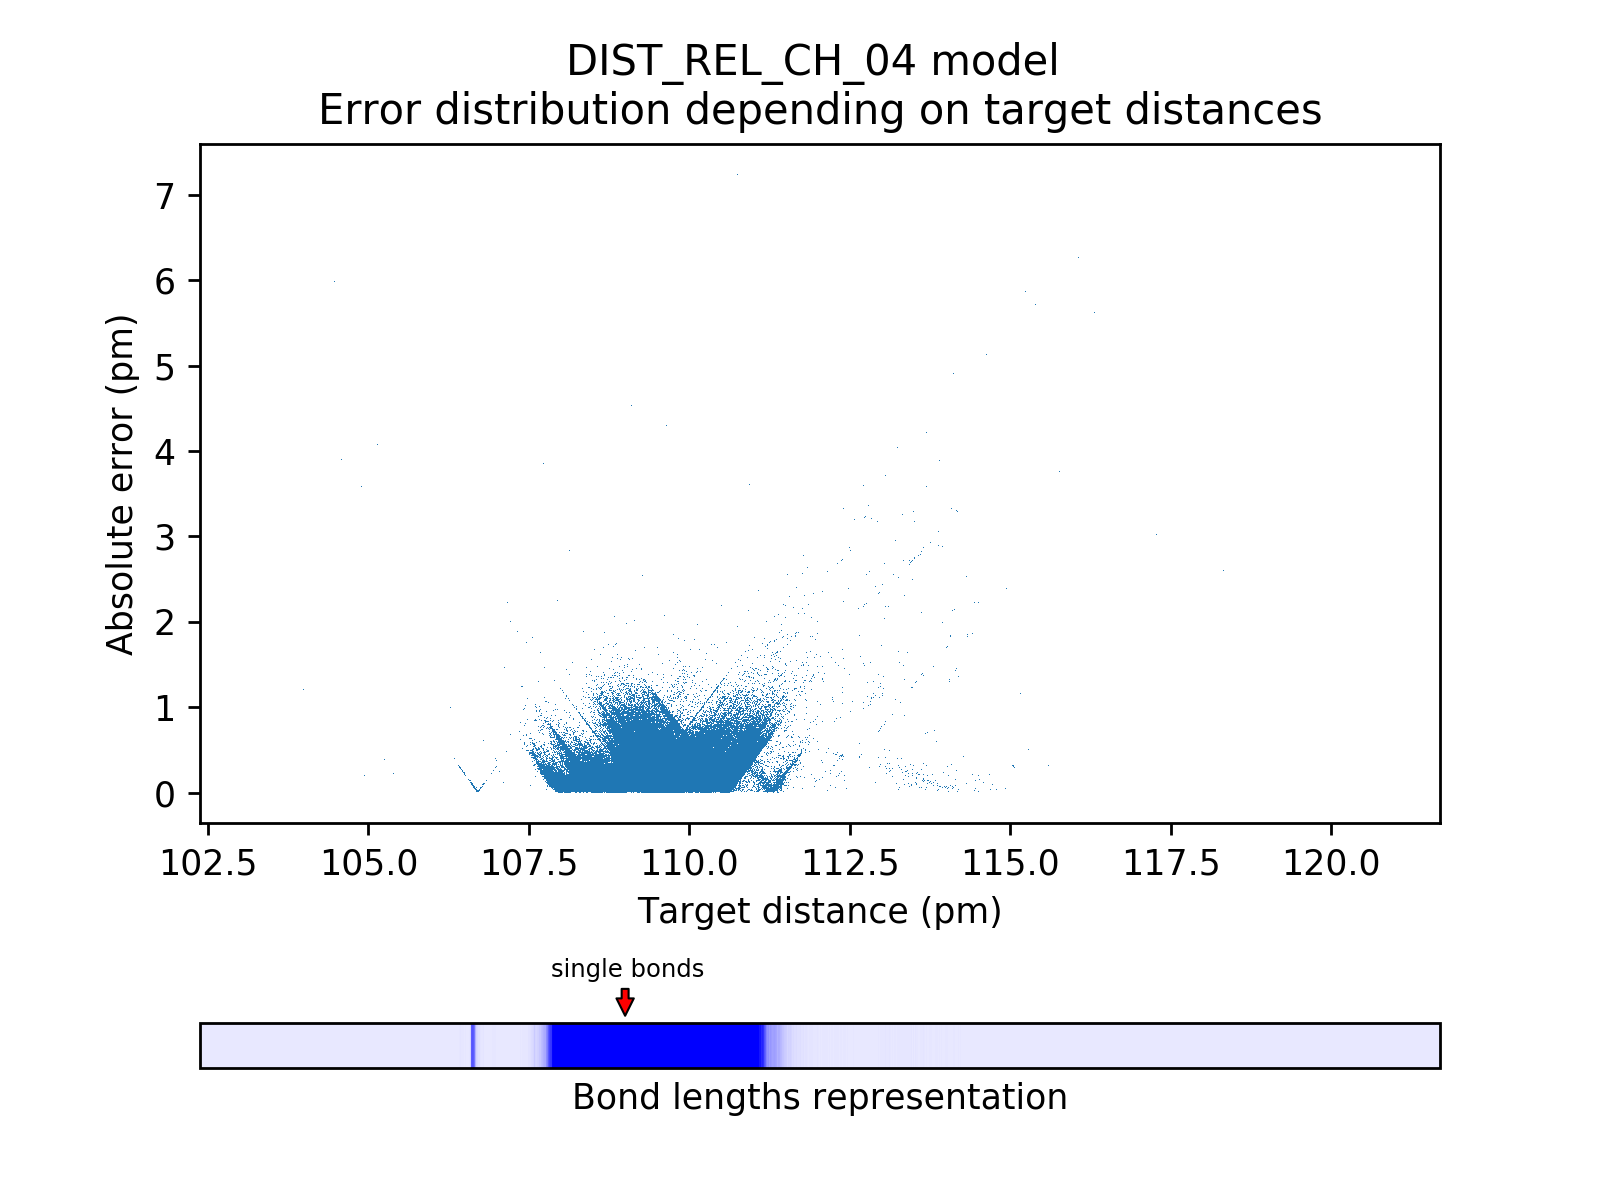
\includegraphics[scale=0.75]{../figures/DIST_REL_CH_04/DIST_REL_CH_04_distrib_rmse_dist.png}	
	
	\caption{Erreur en fonction des cibles pour le modèle \emph{DIST\_REL\_CH\_04}. Modèle s'entraînant sur une \textbf{grande quantité d'exemples} et prédisant les longueurs de liaisons \textbf{carbone-hydrogene}, à partir de données d'entrées sur lesquelles la \textbf{fonction inverse} a été appliquée aux distances, \textbf{avec restriction} au voisinage le plus proche.}
\end{figure}

\begin{figure}[!h]
	\centering
	
	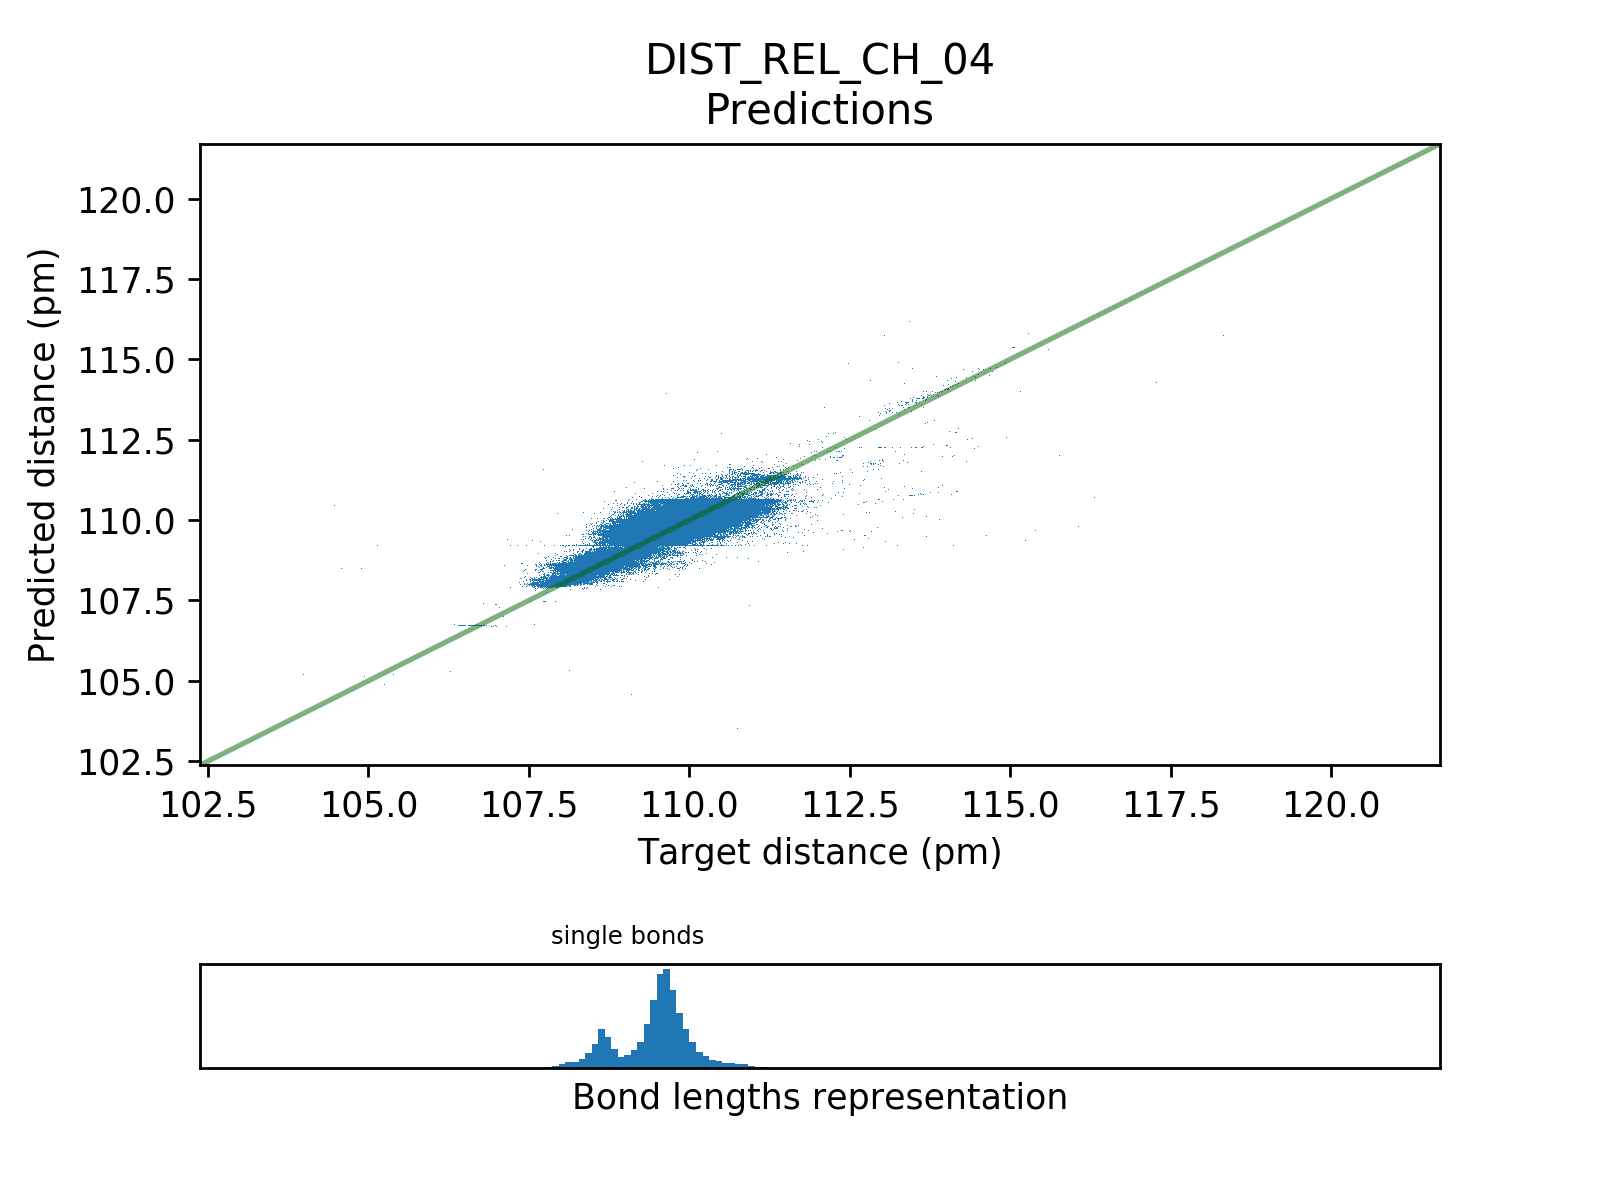
\includegraphics[scale=0.75]{../figures/DIST_REL_CH_04/DIST_REL_CH_04_preds_targets.png}	
	
	\caption{Prédictions en fonction des cibles pour le modèle \emph{DIST\_REL\_CH\_04}. Modèle s'entraînant sur une \textbf{grande quantité d'exemples} et prédisant les longueurs de liaisons \textbf{carbone-hydrogene}, à partir de données d'entrées sur lesquelles la \textbf{fonction inverse} a été appliquée aux distances, \textbf{avec restriction} au voisinage le plus proche.}
	
\end{figure}

% DIST REL OH 04

\begin{figure}[!h]
	\centering
	
	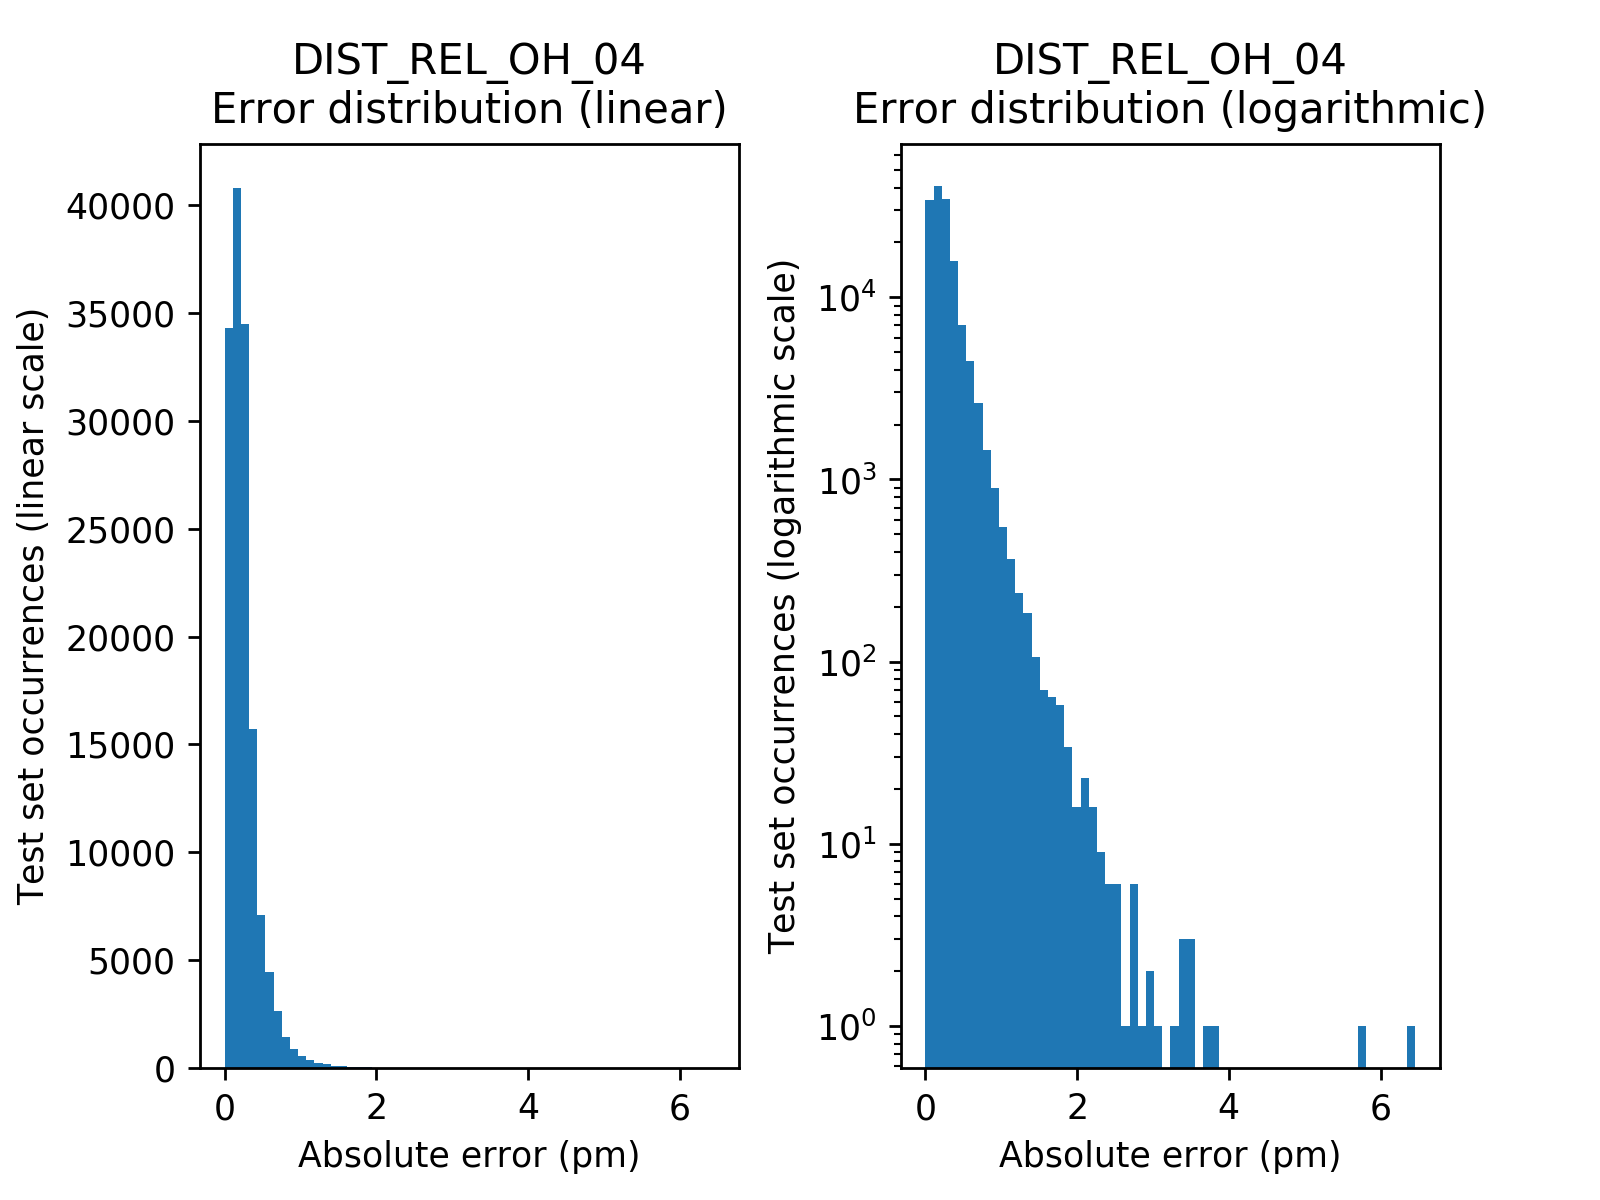
\includegraphics[scale=0.75]{../figures/DIST_REL_OH_04/DIST_REL_OH_04_distrib_rmse_val.png}	
	
	\caption{Distribution des erreurs du modèle \emph{DIST\_REL\_OH\_04}. Modèle s'entraînant sur une \textbf{grande quantité d'exemples} et prédisant les longueurs de liaisons \textbf{oxygène-hydrogene}, à partir de données d'entrées sur lesquelles la \textbf{fonction inverse} a été appliquée aux distances, \textbf{avec restriction} au voisinage le plus proche.}
\end{figure}

\begin{figure}[!h]
	\centering
	
	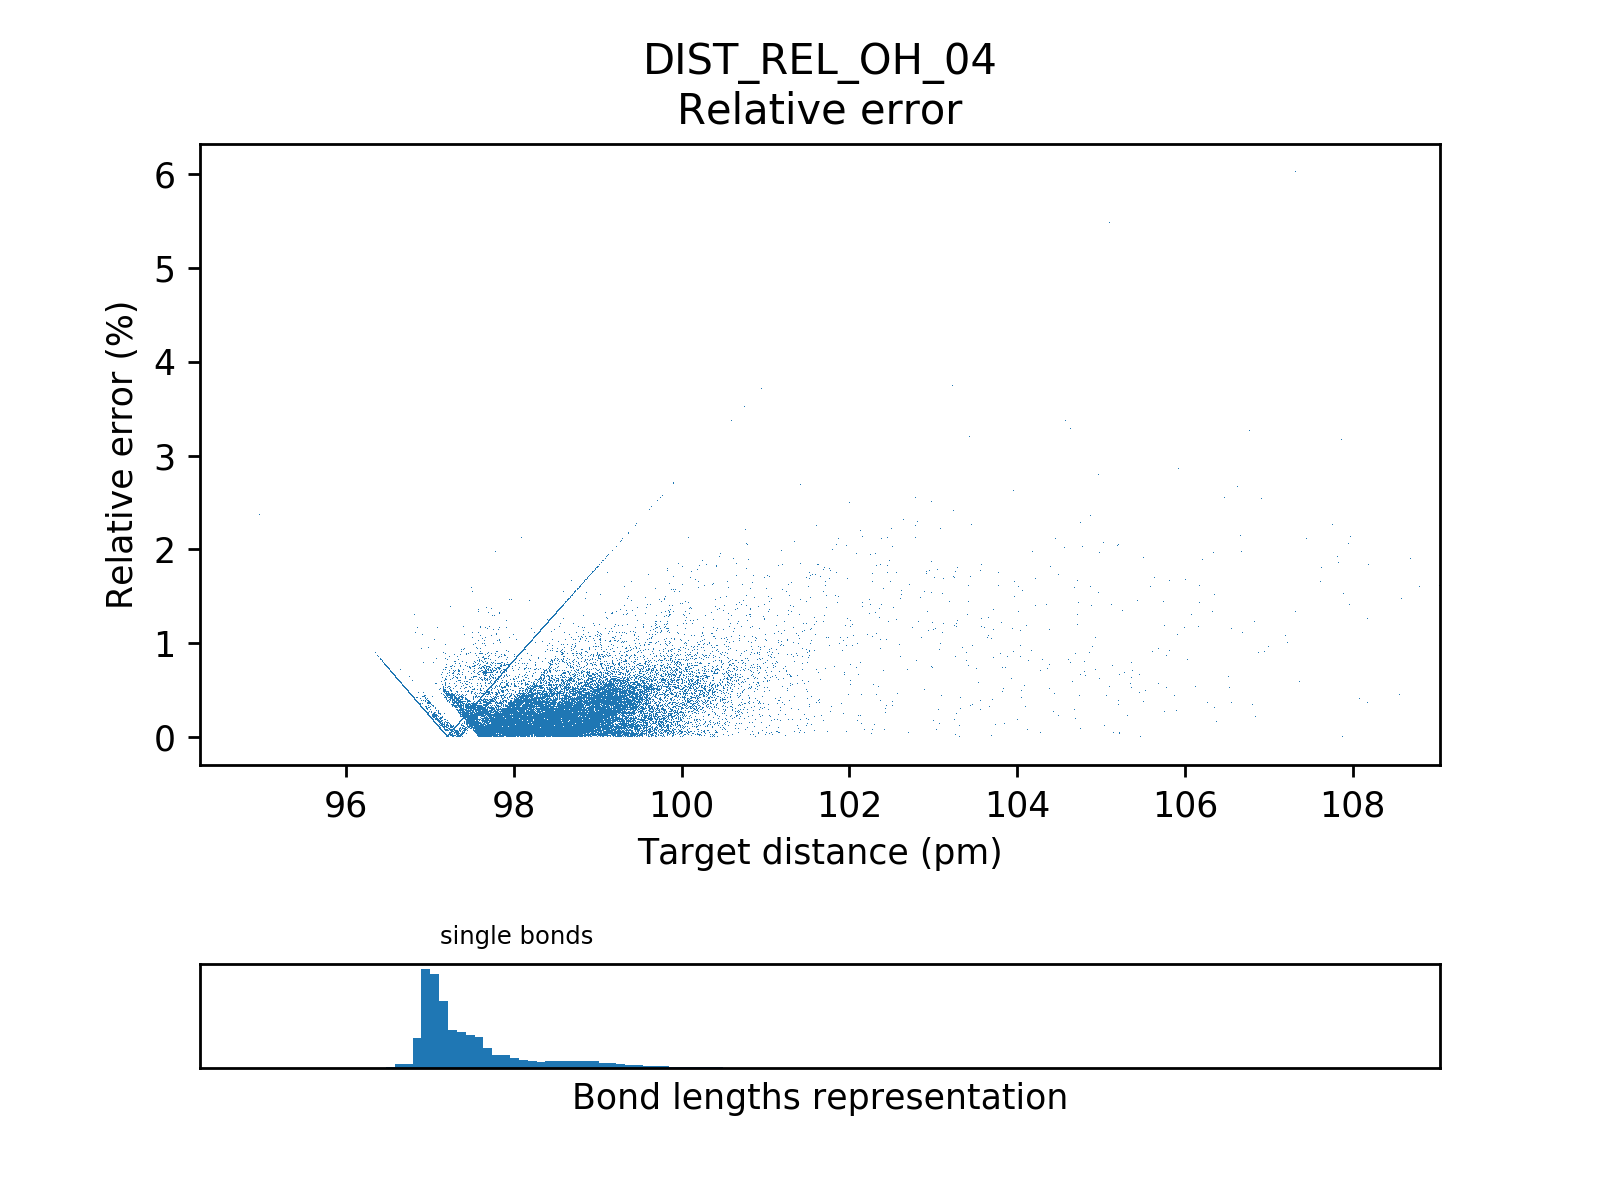
\includegraphics[scale=0.75]{../figures/DIST_REL_OH_04/DIST_REL_OH_04_distrib_rmse_dist.png}	
	
	\caption{Erreur en fonction des cibles pour le modèle \emph{DIST\_REL\_OH\_04}. Modèle s'entraînant sur une \textbf{grande quantité d'exemples} et prédisant les longueurs de liaisons \textbf{oxygène-hydrogene}, à partir de données d'entrées sur lesquelles la \textbf{fonction inverse} a été appliquée aux distances, \textbf{avec restriction} au voisinage le plus proche.}
\end{figure}

\begin{figure}[!h]
	\centering
	
	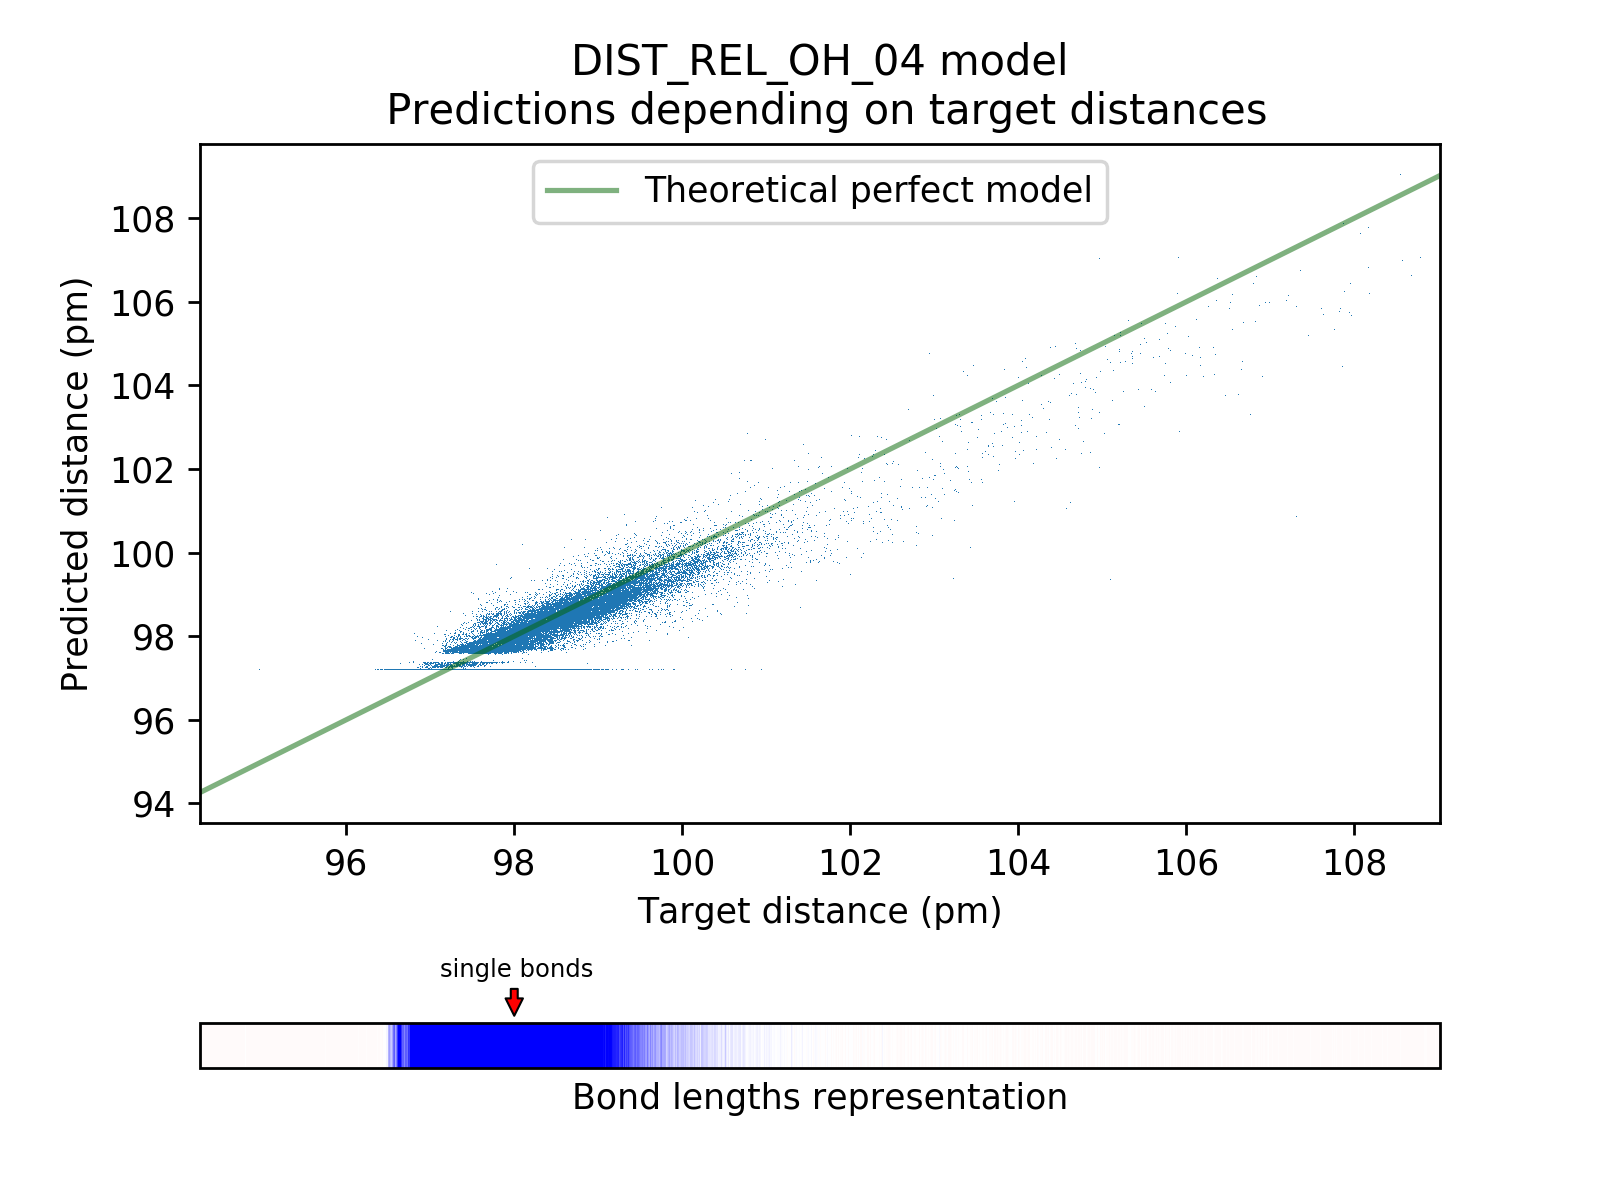
\includegraphics[scale=0.75]{../figures/DIST_REL_OH_04/DIST_REL_OH_04_preds_targets.png}	
	
	\caption{Prédictions en fonction des cibles pour le modèle \emph{DIST\_REL\_OH\_04}. Modèle s'entraînant sur une \textbf{grande quantité d'exemples} et prédisant les longueurs de liaisons \textbf{oxygène-hydrogene}, à partir de données d'entrées sur lesquelles la \textbf{fonction inverse} a été appliquée aux distances, \textbf{avec restriction} au voisinage le plus proche.}
	
\end{figure}

\chapter{Résultats de la recherche par quadrillage du modèle KRR}

\label{annexes_krr_quadri}

\begin{verbatim}

0.935 (+/-0.007) for {'coef0': 1, 'kernel': 'linear', 'degree': 1, 'gamma': None, 'alpha': 0.1}
0.726 (+/-0.292) for {'coef0': 1, 'kernel': 'linear', 'degree': 1, 'gamma': None, 'alpha': 0.01}
0.615 (+/-0.495) for {'coef0': 1, 'kernel': 'linear', 'degree': 1, 'gamma': None, 'alpha': 0.001}
0.935 (+/-0.011) for {'coef0': 1, 'kernel': 'poly', 'degree': 2, 'gamma': None, 'alpha': 0.1}
0.817 (+/-0.285) for {'coef0': 1, 'kernel': 'poly', 'degree': 6, 'gamma': None, 'alpha': 0.1}
0.934 (+/-0.012) for {'coef0': 0.5, 'kernel': 'poly', 'degree': 2, 'gamma': None, 'alpha': 0.1}
0.586 (+/-0.772) for {'coef0': 0.5, 'kernel': 'poly', 'degree': 6, 'gamma': None, 'alpha': 0.1}
0.937 (+/-0.010) for {'coef0': 2, 'kernel': 'poly', 'degree': 2, 'gamma': None, 'alpha': 0.1}
0.899 (+/-0.124) for {'coef0': 2, 'kernel': 'poly', 'degree': 6, 'gamma': None, 'alpha': 0.1}
0.951 (+/-0.006) for {'coef0': 1, 'kernel': 'poly', 'degree': 2, 'gamma': None, 'alpha': 0.01}
0.760 (+/-0.384) for {'coef0': 1, 'kernel': 'poly', 'degree': 6, 'gamma': None, 'alpha': 0.01}
0.950 (+/-0.007) for {'coef0': 0.5, 'kernel': 'poly', 'degree': 2, 'gamma': None, 'alpha': 0.01}
0.703 (+/-0.312) for {'coef0': 0.5, 'kernel': 'poly', 'degree': 6, 'gamma': None, 'alpha': 0.01}
0.951 (+/-0.006) for {'coef0': 2, 'kernel': 'poly', 'degree': 2, 'gamma': None, 'alpha': 0.01}
0.909 (+/-0.107) for {'coef0': 2, 'kernel': 'poly', 'degree': 6, 'gamma': None, 'alpha': 0.01}
0.917 (+/-0.049) for {'coef0': 1, 'kernel': 'poly', 'degree': 2, 'gamma': None, 'alpha': 0.001}
0.742 (+/-0.394) for {'coef0': 1, 'kernel': 'poly', 'degree': 6, 'gamma': None, 'alpha': 0.001}
0.942 (+/-0.004) for {'coef0': 0.5, 'kernel': 'poly', 'degree': 2, 'gamma': None, 'alpha': 0.001}
0.699 (+/-0.330) for {'coef0': 0.5, 'kernel': 'poly', 'degree': 6, 'gamma': None, 'alpha': 0.001}
0.935 (+/-0.012) for {'coef0': 2, 'kernel': 'poly', 'degree': 2, 'gamma': None, 'alpha': 0.001}
0.895 (+/-0.146) for {'coef0': 2, 'kernel': 'poly', 'degree': 6, 'gamma': None, 'alpha': 0.001}
Best score: 0.951
Best parameters set:
{'kernel_params': None, 'kernel': 'poly', 'degree': 2, 'gamma': None, 'alpha': 0.01, 'coef0': 1}
\end{verbatim}


\begin{landscape}

\chapter{Paramètres des modèles \emph{DELTA\_DIST\_+H}}

\label{annexes_param_delta_dist}

\centering

\begin{tabular}{|c|c|c|c|c|c|c|c|c|c|c|c|}
\hline
\begin{minipage}{3.5cm} \vspace{5mm}Modèle\vspace{5mm}\end{minipage} & 
\begin{minipage}{1.3cm}Tailles \\molécules\end{minipage} & 
\begin{minipage}{1.8cm}Repr. géom.\\ entrée\end{minipage} & 
\begin{minipage}{1.8cm}Repr. géom.\\ sortie \end{minipage} & 
\begin{minipage}{1.4cm}Numéros\\ atomiques \end{minipage} & 
\begin{minipage}{1.4cm}Masses\\ atomiques \end{minipage} &
\begin{minipage}{2cm}Distances inter at. fictifs \end{minipage} & 
\begin{minipage}{1.8cm}Fonction de coût \end{minipage} & 
\begin{minipage}{1.65cm}Profondeur \end{minipage} & 
\begin{minipage}{1.2cm}Largeur \end{minipage} & 
\begin{minipage}{1cm}Taille\\ entrée \end{minipage} & 
\begin{minipage}{0.9cm}Bruit \end{minipage} \\  \hline

\begin{minipage}{3.5cm}\vspace{5mm}DELTA\_DIST+H\_01 \vspace{1mm} \end{minipage} &
\begin{minipage}{1.3cm}0 - 200 \end{minipage} &
\begin{minipage}{1.8cm}Matr. dist. pts. fixes \end{minipage} &
\begin{minipage}{1.8cm}Matr. dist. pts. fixes \end{minipage} &
\begin{minipage}{1.4cm}Non \end{minipage} &
\begin{minipage}{1.4cm}Oui \end{minipage} &
\begin{minipage}{2cm} Non \end{minipage} &
\begin{minipage}{1.8cm}RMSE\\ partiel/total \end{minipage}&
\begin{minipage}{1.65cm} 4 \end{minipage}&
\begin{minipage}{1.2cm} 8650 \end{minipage} &
\begin{minipage}{1cm}1000 \end{minipage} &
\begin{minipage}{0.9cm}+/++ \end{minipage} \\  \hline

\begin{minipage}{3.5cm}\vspace{5mm}DELTA\_DIST+H\_02 \vspace{1mm} \end{minipage} &
\begin{minipage}{1.3cm}0 - 200 \end{minipage} &
\begin{minipage}{1.8cm}Matr. dist. pts. fixes \end{minipage} &
\begin{minipage}{1.8cm}Matr. dist. pts. fixes \end{minipage} &
\begin{minipage}{1.4cm}Non \end{minipage} &
\begin{minipage}{1.4cm}Oui \end{minipage} &
\begin{minipage}{2cm} Oui \end{minipage} &
\begin{minipage}{1.8cm}RMSE\\ partiel \end{minipage}&
\begin{minipage}{1.65cm} 4 \end{minipage}&
\begin{minipage}{1.2cm} 8650 \end{minipage} &
\begin{minipage}{1cm}1020 \end{minipage} &
\begin{minipage}{0.9cm}+ \end{minipage} \\  \hline

\begin{minipage}{3.3cm}\vspace{1cm}DELTA\_DIST+H\_03 \vspace{5mm} \end{minipage} &
\begin{minipage}{1.3cm}0 - 200 \end{minipage} &
\begin{minipage}{1.8cm}Matr. dist. pts. fixes + \\ Matr red. dist. inter-at. \end{minipage} &
\begin{minipage}{1.8cm}Matr. dist. pts. fixes \end{minipage} &
\begin{minipage}{1.4cm}Non \end{minipage} &
\begin{minipage}{1.4cm}Oui \end{minipage} &
\begin{minipage}{2cm} Non \end{minipage} &
\begin{minipage}{1.8cm}RMSE\\ partiel \end{minipage}&
\begin{minipage}{1.65cm} 3 \end{minipage}&
\begin{minipage}{1.2cm} 9000 \end{minipage} &
\begin{minipage}{1cm}1800\end{minipage} &
\begin{minipage}{0.9cm}++ \end{minipage} \\  \hline

\begin{minipage}{3.5cm}\vspace{1cm}DELTA\_DIST+H\_04 \vspace{5mm} \end{minipage} &
\begin{minipage}{1.3cm}0 - 200 \end{minipage} &
\begin{minipage}{1.8cm}Matr. dist. pts. fixes + \\ Matr red. dist. inter-at. \end{minipage} &
\begin{minipage}{1.8cm} Matr red. dist. inter-at. \end{minipage} &
\begin{minipage}{1.4cm}Non \end{minipage} &
\begin{minipage}{1.4cm}Oui \end{minipage} &
\begin{minipage}{2cm} Non \end{minipage} &
\begin{minipage}{1.8cm}RMSE\\ partiel \end{minipage}&
\begin{minipage}{1.65cm} 3 \end{minipage}&
\begin{minipage}{1.2cm} 9000 \end{minipage} &
\begin{minipage}{1cm}1800\end{minipage} &
\begin{minipage}{0.9cm}++ \end{minipage} \\  \hline


\begin{minipage}{3.5cm}\vspace{1cm}DELTA\_DIST+H\_05 \vspace{5mm} \end{minipage} &
\begin{minipage}{1.3cm}2 - 60 \end{minipage} &
\begin{minipage}{1.8cm}Matr. dist. pts. fixes \end{minipage} &
\begin{minipage}{1.8cm}Matr. dist. pts. fixes \end{minipage} &
\begin{minipage}{1.4cm}Oui \end{minipage} &
\begin{minipage}{1.4cm}Oui \end{minipage} &
\begin{minipage}{2cm} Non \end{minipage} &
\begin{minipage}{1.8cm}RMSE\\ partiel \end{minipage}&
\begin{minipage}{1.65cm} 3 \end{minipage}&
\begin{minipage}{1.2cm} 360 \end{minipage} &
\begin{minipage}{1cm} 360 \end{minipage} &
\begin{minipage}{0.9cm}++ \end{minipage} \\  \hline


\end{tabular}

\end{landscape}